%%____________________________________________________________________________||
\section{Systematic uncertainties in the transfer factors}
\label{sec:systematics}

This section addresses the estimation of systematic uncertainties in
the estimation of event counts from non-multijet backgrounds. This
analysis aims to rely as much as possible on the data control samples
to check for sources of bias in the transfer factors described in
Sec.~\ref{sec:ewk-method} and derive the associated systematic
uncertainties. The strategies that are employed to ascertain the
presence of biases or otherwise, and the procedures used to derive
systematic uncertainties, are described below.

Two types of systematic uncertainty are considered separately. First,
we consider ``normalisation'' uncertainties in the predictions of
background counts in each (\njet,~\nb,~\scalht) bin, integrated over
\mht, of the signal region. Second, systematic uncertainties
associated with the \mht templates obtained from simulation for each
individual (\njet,~\nb,~\scalht) bin are determined from multiple data
control samples. The determination and validation of the \mht
templates and their associated uncertainties are described fully in
Sec.~\ref{sec:syst-on-shape}.

This chapter covers in detail the normalisation systematic
uncertainties associated with predictions per (\njet,~\nb,~\scalht)
bins. Sec.~\ref{sec:mc-systematics} outlines simulation-based studies of the
effects of potential sources of bias on the transfer factors.
The use of ``closure tests'' to derive additional, data driven, systematic
uncertainties are described in detail in Secs.~\ref{sec:bkgdnorm-syst}
and \ref{sec:syst-from-closure}. The definition of tests geared
towards the specific background processes are outlined. The observed level 
of closure in data
and the resulting systematic uncertainties, based on control samples
corresponding to $2.1~\ifb$ of integrated luminosity are shown.
% Further dedicated closure tests that
% provide additional cross checks are covered in
% Sec.~\ref{sec:closureCrossCheck}. 

%%%%%%%%%%%%%%%%%%%%%%%%%%%%%%%%%%%%%%%%%%%%%%%%%%%%%%%%%%%%%%%%
% MC systs
%%%%%%%%%%%%%%%%%%%%%%%%%%%%%%%%%%%%%%%%%%%%%%%%%%%%%%%%%%%%%%%%

\subsection{Simulation-based studies of normalisation systematic uncertainties}
\label{sec:mc-systematics}

As described in Secs.~\ref{sec:backgroundmet}, the non-multijet background yields
per $(\njet,\nb,\scalht)$ bin are estimated through the use of control
regions and appropriate MC-based transfer factors. This approach aims
to minimise the sensitivity to simulation mismodelling, as many
systematic biases are expected to cancel to a large extent in the
ratios defining the transfer factors. However, residual biases may
still remain if problems in the simulation are equivalently modelled
in the numerator and denominator of the transfer factors. To address
and quantify these uncertainties the effect of the transfer factors is
observed after appropriately varying MC yields based on relevant
uncertainties. These investigations are presented in this section. 

We consider a wide range of systematic effects arising from
uncertainties in jet energy scales, b-tag scale factors, pileup
reweighting, top $p_T$ reweighting lepton and photon identification, etc. 
On top of the MC studies, additional data-driven systematic 
uncertainties are derived from closure tests, described in
Sec.~\ref{sec:closure-tests}.

The procedure to determine the effect of these sources of systematic
uncertainties is to construct the transfer factors when varying in
turn each source by their up and down one sigma uncertainties, and
express this as a percentage difference relative to the nominal
transfer factors. These systematics are encoded in the likelihood
model as shape uncertainties where the parameter is fully correlated
but with a different magnitude in each \njet,\nb and \scalht bin.

These sources of systematic uncertainty can effect both the
experimental acceptance of the signal and control regions, as well as
event migration between analysis bins. 
%The former is accounted for by cross section corrections derived from
%sidebands and NNLO calculations. 
The aim in this case is to assess the relative changes in the transfer
factors across bins as the variations are performed and the overall
integrated yields are fixed.

\subsubsection{Jet energy corrections}

The effect of varying the jet energy scale in
the \mj and \mmj control regions is investigated.  The energies of
jets used in the analysis are corrected as a function of their \pt and
$\eta$ via the procedure recommended by the JetMET POG. These
corrections have an associated uncertainty, which can propagate
through the analysis.  As the analysis is designed such that bins with
the same value of \scalht and jet multiplicity in the control regions
are used to predict the background in the signal region, this analysis
expects to be protected against many of the effects caused by these jet energy
scale uncertainties. However, the jet energy scale can still have an
effect, due to jets moving in and out acceptance (above and below
$40\gev$).

Full selection, as described in Sec.~\ref{sec:selection}, is required.
If any control region bin has fewer than $1$ predicted events at
$1280\ipb$ it is left out of the study.  Pseudo transfer factors are
calculated in each analysis bin, defined as the number of events in a
signal region after passing the signal region \alphat cut in a
particular bin divided by the total number of events in that bin. This
is carried out using the jet energy corrections with their nominal,
most likely, value and with their minus one sigma, lower bound,
value. The relative change in these two transfer factors is then
calculated. For the \mj control region, these values are shown in
Fig.~\ref{fig:jes-syst-singleMu}. For the \mmj control region, these
values are shown in Fig.~\ref{fig:jes-syst-doubleMu}.

Overall, the effect of varying the jet energy scale down appears to be
small. With variations in the pseudo transfer factors being typically
less than $10\%$. Any larger effects are likely due to statistical
fluctuations in bins with a small number of events.

\subsubsection{b-tagging efficiency scale factors}

Scale factors provided by the BTV POG are applied to the MC samples
to correct for differences in the b-tagging efficiencies and 
misidentifications between simulation and data. The method employed is
based on simple event reweighting as described in
Ref.~\cite{btagSFMethods}. Events are reweighted according to the
probability of obtaining a particular jet configuration in data
and simulation, as determined by the b-tagging efficiencies computed
in the MC samples and the scale factors measured in data.

Figure ~\ref{fig:btagSF-syst-singleMu} shows the effect on the transfer
factors in the \mj control region of varying the b-tag scale factors 
up and down by their corresponding uncertainties. The systematic
effect is very small, at the percent level or less, and is
sub-dominant with respect to the systematic errors derived from the 
closure tests.

\subsubsection{Pileup reweighting}

As the distribution of pileup events differs between simulation and
data a reweighting is carried out as described in
Sec.~\ref{sec:pileup-reweighting}. There is an uncertainty associated
with the reweighting factors. The factors are therefore varied based
on this uncertainty and the effect of the variation included as a
systematic uncertainty on the transfer factors.

\subsubsection{Top $p_T$ reweighting}

Variations in the reweighting top $p_{T}$ distribution, as first outlined in 
Sec.~\ref{sec:SMxs}, are studied and the effect on the transfer
factors used to determine a systematic uncertainty.

\subsubsection{QCD contamination}

A check has also been performed on the systematic effect on the
background prediction due to QCD contamination in the control samples,
which has been found to be at the percent level for the \mj and \gj
control regions. Applying an arbitrarily large variation of $\pm
100\%$ on the number of Monte Carlo QCD events leads to a systematic
variation on the transfer factors of at most 5\% in the majority of
bins.

This preliminary study suggest that effects from the QCD
uncertainties are small and should be covered by other systematics
(particularly those derived from the closure tests in
Sec.~\ref{sec:closure-tests}).


%%%%%%%%%%%%%%%%%%%%%%%%%%%%%%%%%%%%%%%%%%%%%%%%%%%%%%%%%%%%%%%%
% Closure tests
%%%%%%%%%%%%%%%%%%%%%%%%%%%%%%%%%%%%%%%%%%%%%%%%%%%%%%%%%%%%%%%%

\subsection{Data driven systematics with closure tests}
\label{sec:closure-tests}

\subsubsection{Definition of a closure test}
\label{sec:closure-tests-desc}

Along with the MC variation tests described in Sec.~\ref{sec:mc-systematics}, 
the sensitivity of the transfer factors to potential limitations in
the simulation modelling is established through sets of closure tests.
These tests confront data yields measured in one data control (sub-)sample
against the predictions determined from another data control
(sub-)sample as a function of \scalht. An extrapolation is made
from one control (sub-)sample to another (rather than to the signal
region) in bins of \scalht via transfer factors determined from
simulation. 

The level of statistical consistency between the predicted and
observed yields of each closure test in the ensemble is inspected. The
agreement between the predicted and observed yields is
expressed as the ratio $(\nobs - \npre)/\npre$ while considering only
the statistical uncertainties on \npre and \nobs. Therefore, the level
of closure is defined by the statistical significance of a deviation
in the ratio from zero. A ``set'' of closure tests includes
statistically independent tests determined as a function of \scalht
and \njet (according to the \scalht and \njet binning used in the control and signal
regions), in most cases integrated over \nb. In this way, a set of closure 
tests allows one to establish
the presence of significant biases or dependence on
\scalht or \njet. Importantly, if statistically significant biases are
observed, further studies are required to understand and correct for
these biases. 

Under the assumption of closure for each test of the set,
systematic uncertainties on the transfer factors are derived for each
(\njet,~\nb) category and \scalht bin. The treatment for estimating
the systematic uncertainties on the transfer factors is described in
Sec.~\ref{sec:syst-from-closure}.

The closure tests rely on the \mj, \mmj, and \gj control samples,
as defined in Secs.~\ref{subsec:mucontrolSelection},
\ref{subsec:mumucontrolSelection}, and
\ref{subsec:photoncontrolSelection}. (The \ej and \eej control samples
are not currently used.)

\subsubsection{Systematic uncertainties from closure tests\label{sec:syst-from-closure}}

Each set of closure tests should demonstrate in data, within the
statistical precision of each test, that there are no significant
biases or dependencies on \njet nor \scalht inherent in the transfer
factors obtained from simulation. 
Once it is established that no significant bias or trend is observed
for any set of closure tests, the systematic uncertainties associated
with the transfer factors are determined from tests per \scalht bin
integrated over the \njet dimension. The statistical precision of the 
closure tests are considered
when determining the systematic uncertainties that are assigned to the
transfer factors, as it is only the statistical uncertainties
associated with the tests that limit our knowledge of whether closure
is actually achieved or otherwise. 

The systematic uncertainties in the transfer factors are considered as
a ``normalisation'' uncertainty in the SM background predictions,
which are determined per \scalht bin and are
assumed to be fully correlated between the different (\njet,\nb)
categories and fully uncorrelated between the different \scalht bins. 
Further details or the likelihood model
are provided in Section \ref{sec:likelihood}. The systematic
uncertainty is estimated by taking the quadrature sum of the 
mean and the propagated statistical error for the tests integrated
over \njet in each \scalht bin.

In order to find ``expected systematics'' from the closure tests, \nobs and \npre are
determined from the same sample of simulated events (that guarantees
closure) with statistical uncertainties errors are taken from the
unweighted and weighted counts, respectively. 

We note the behaviour of the magnitude of the systematic uncertainties
on the integrated luminosity, which reduce with increasing
luminosity. This is a reflection of the fully statistical nature of
the ``systematic'' in the absence of bias.

\subsection{Systematic uncertainties for the \znunu background
prediction}

The control of the \znunu\ + jets background, established via the
tests described below, are also validated with the full Run~1 data set
at $\sqrt{s} = 8\tev$, as described in
Appendix~\ref{app:zInvBgControl}.

\subsubsection{Tests probing the prediction of the \znunu
background with the \mj control sample}
\label{sec:muZnunu}

{\bf Variations on the transfer factors from simulation}

All the MC variations described in Sec~\ref{sec:mc-systematics} are
carried out for the transfer factors from the \mj control region to
the \znunu background prediction. The results are shown in
Fig.~\ref{fig:muZnunuTF}.

\begin{figure}[]
  \centering
  \subfigure[Jet energy scale varied up]{
    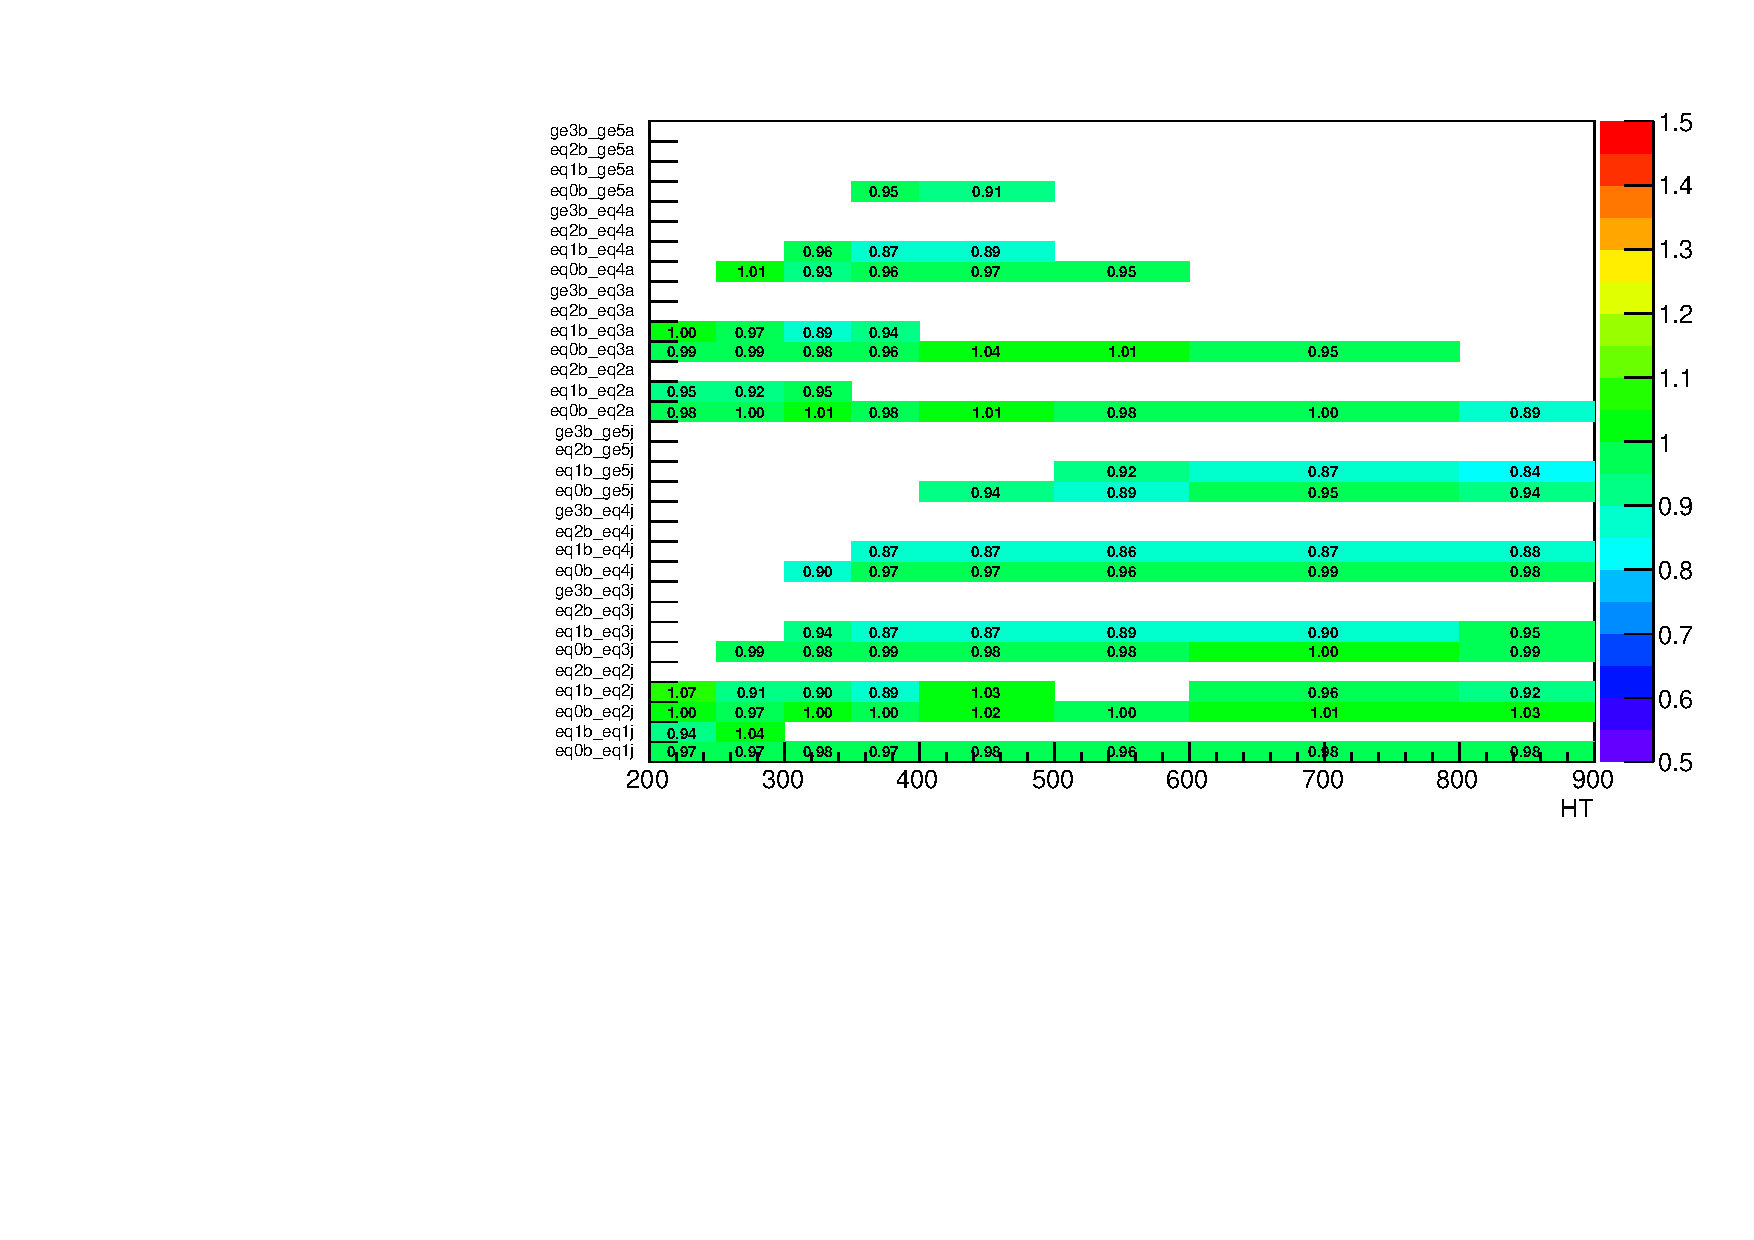
\includegraphics[width=0.5\textwidth]{figures/mcSystematics/Zinv/mu/ratiotfh_ht_mht_alljecWeight_Up.pdf}
  } ~~
  \subfigure[Jet energy scale varied down]{
    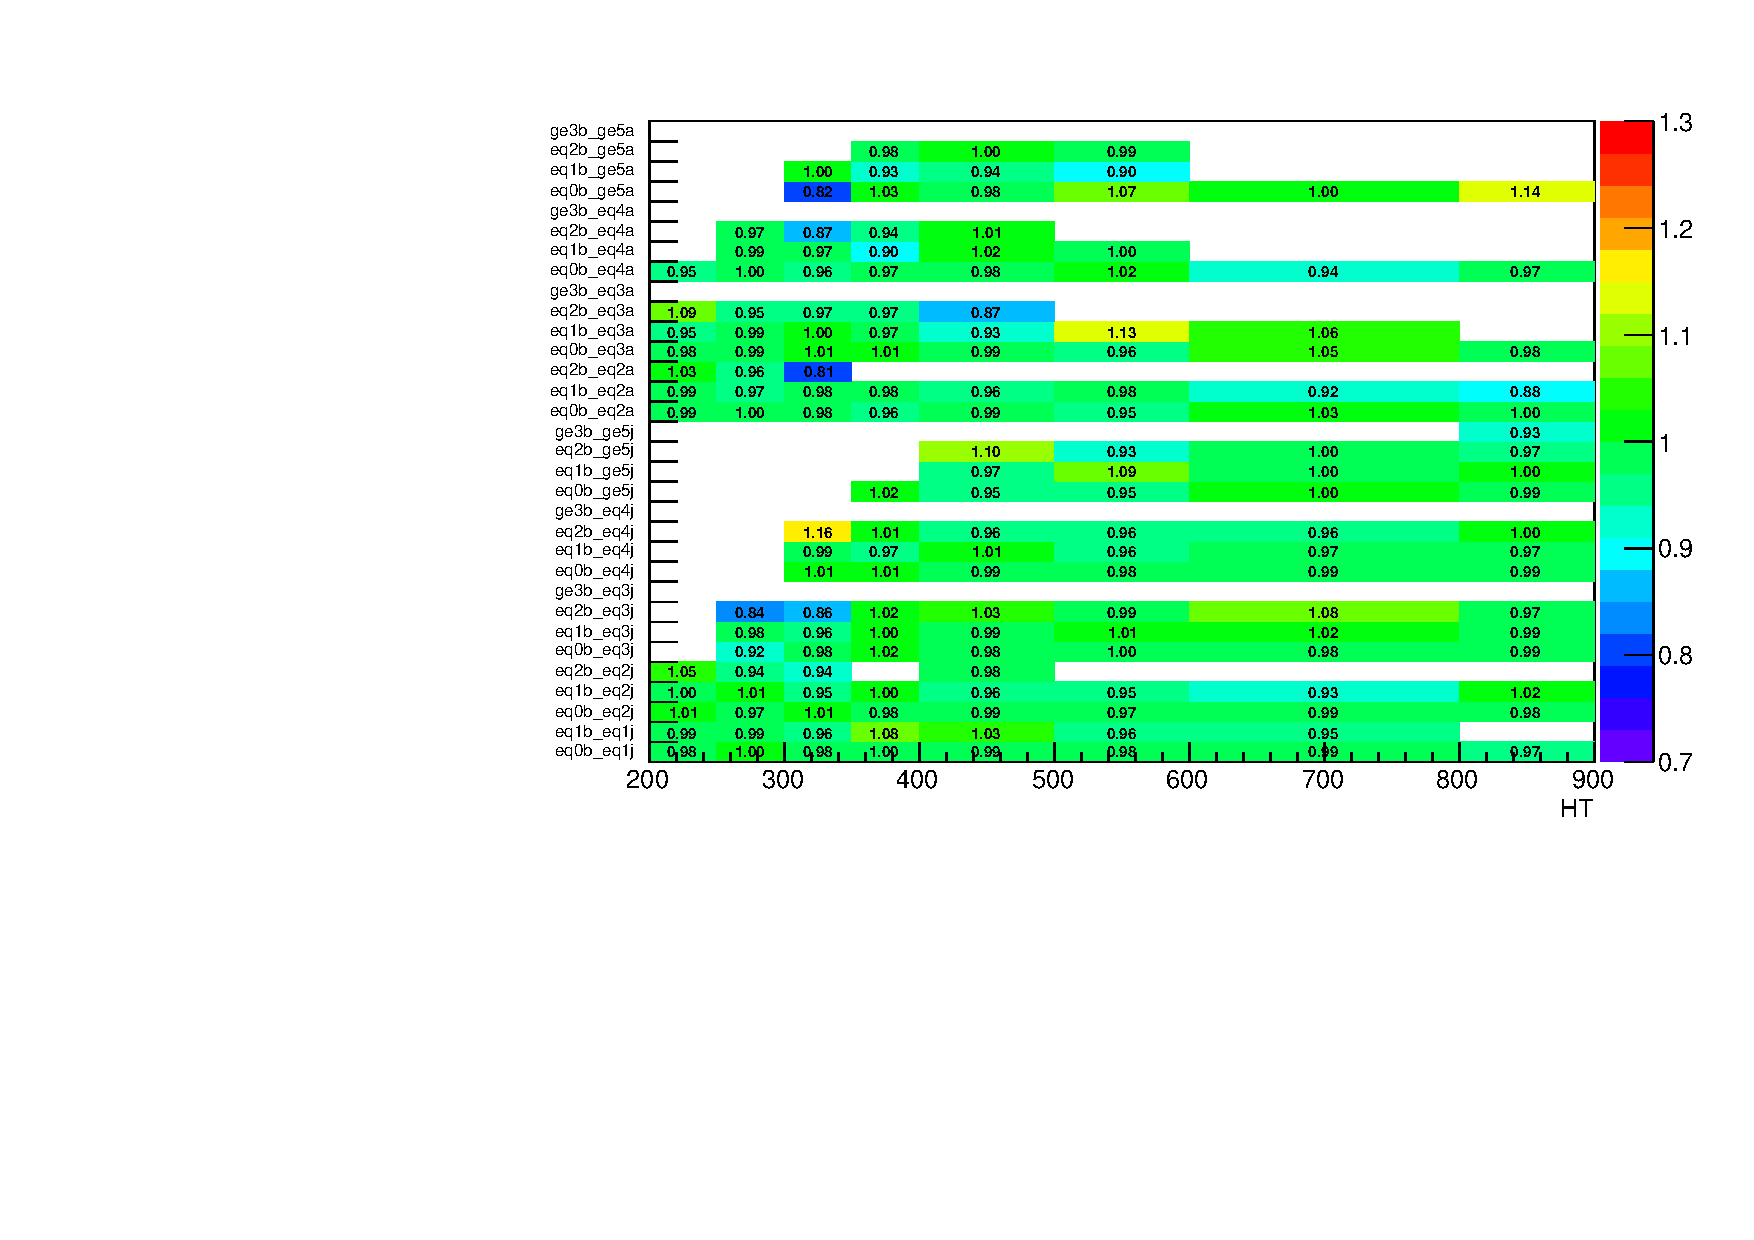
\includegraphics[width=0.5\textwidth]{figures/mcSystematics/Zinv/mu/ratiotfh_ht_mht_alljecWeight_Down.pdf}
  }\\
  \subfigure[B-tag scale factors varied up]{
    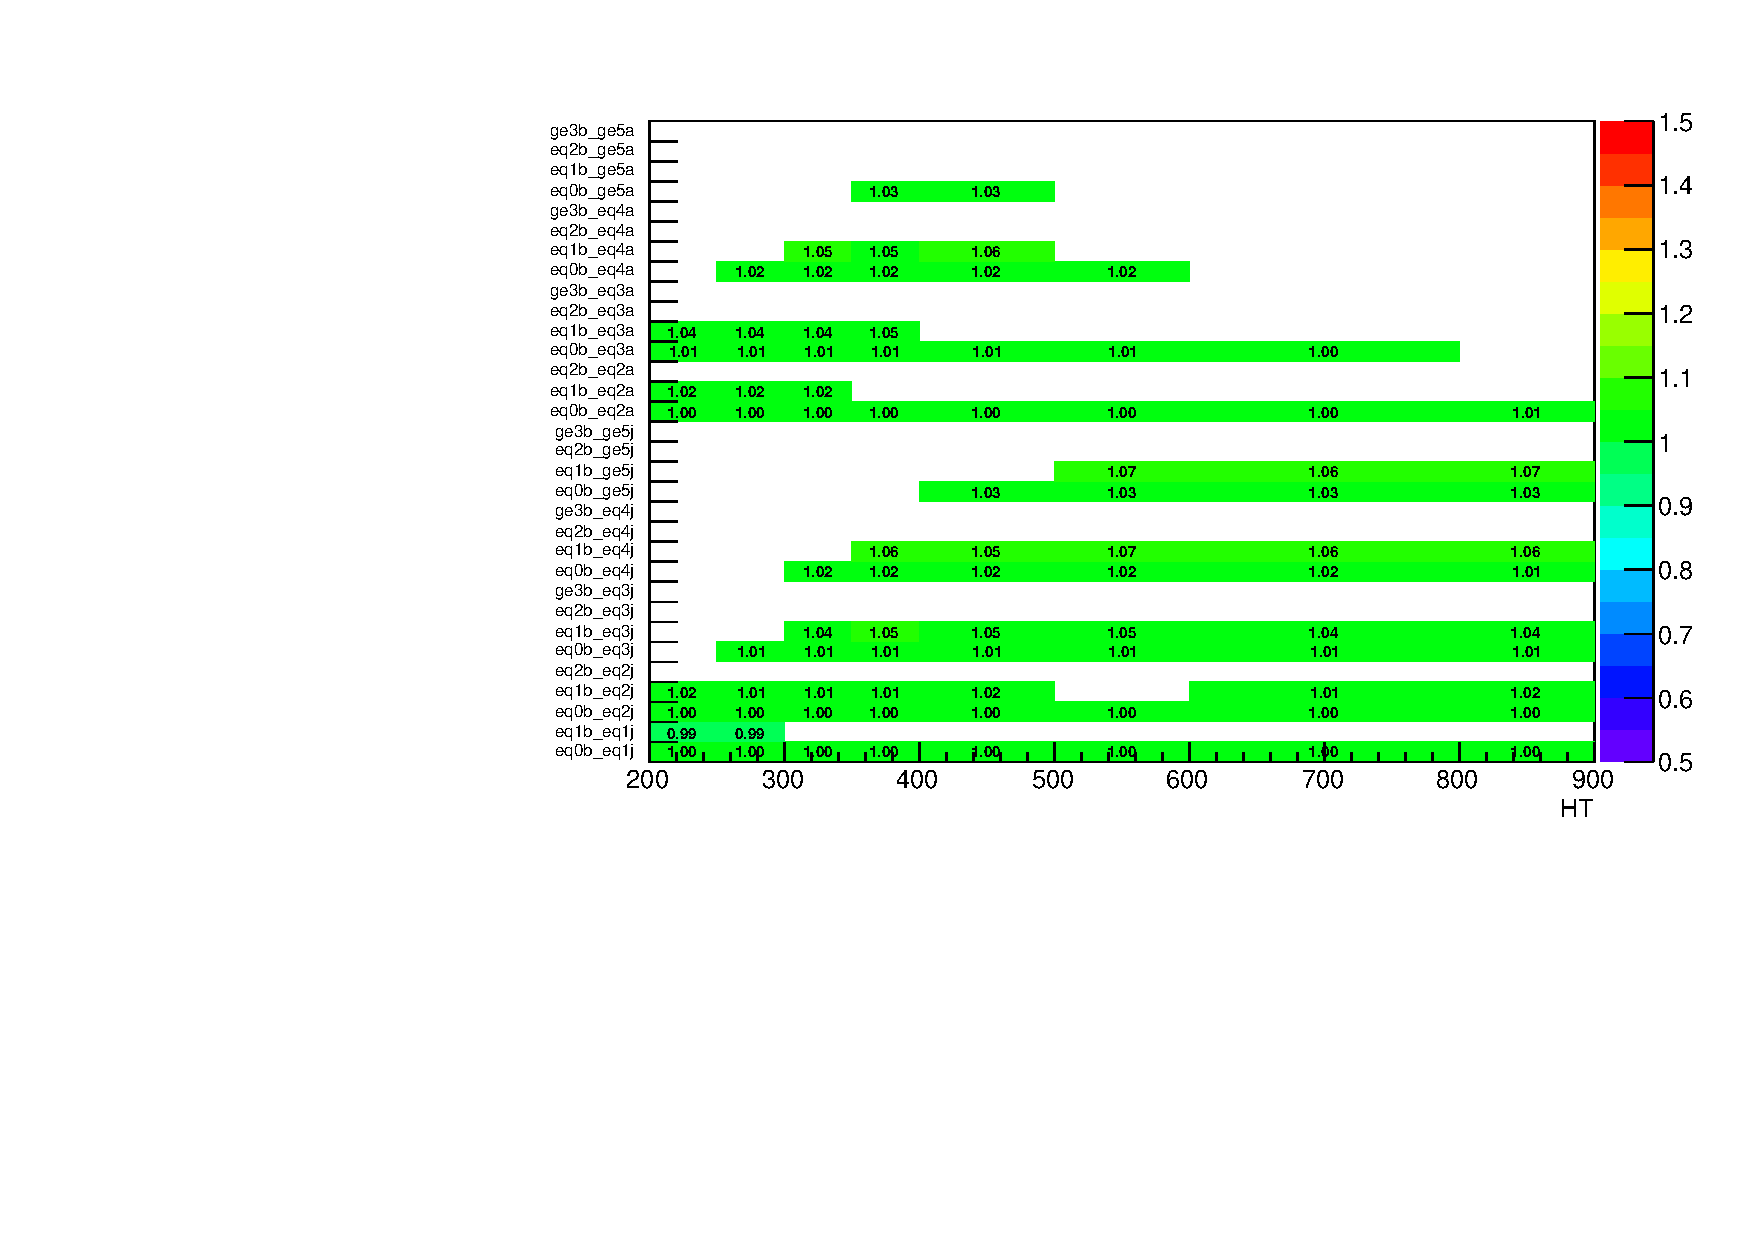
\includegraphics[width=0.5\textwidth]{figures/mcSystematics/Zinv/mu/ratiotfh_ht_mht_allbsfWeight_Up.pdf}
  } ~~
  \subfigure[B-tag scale factors varied down]{
    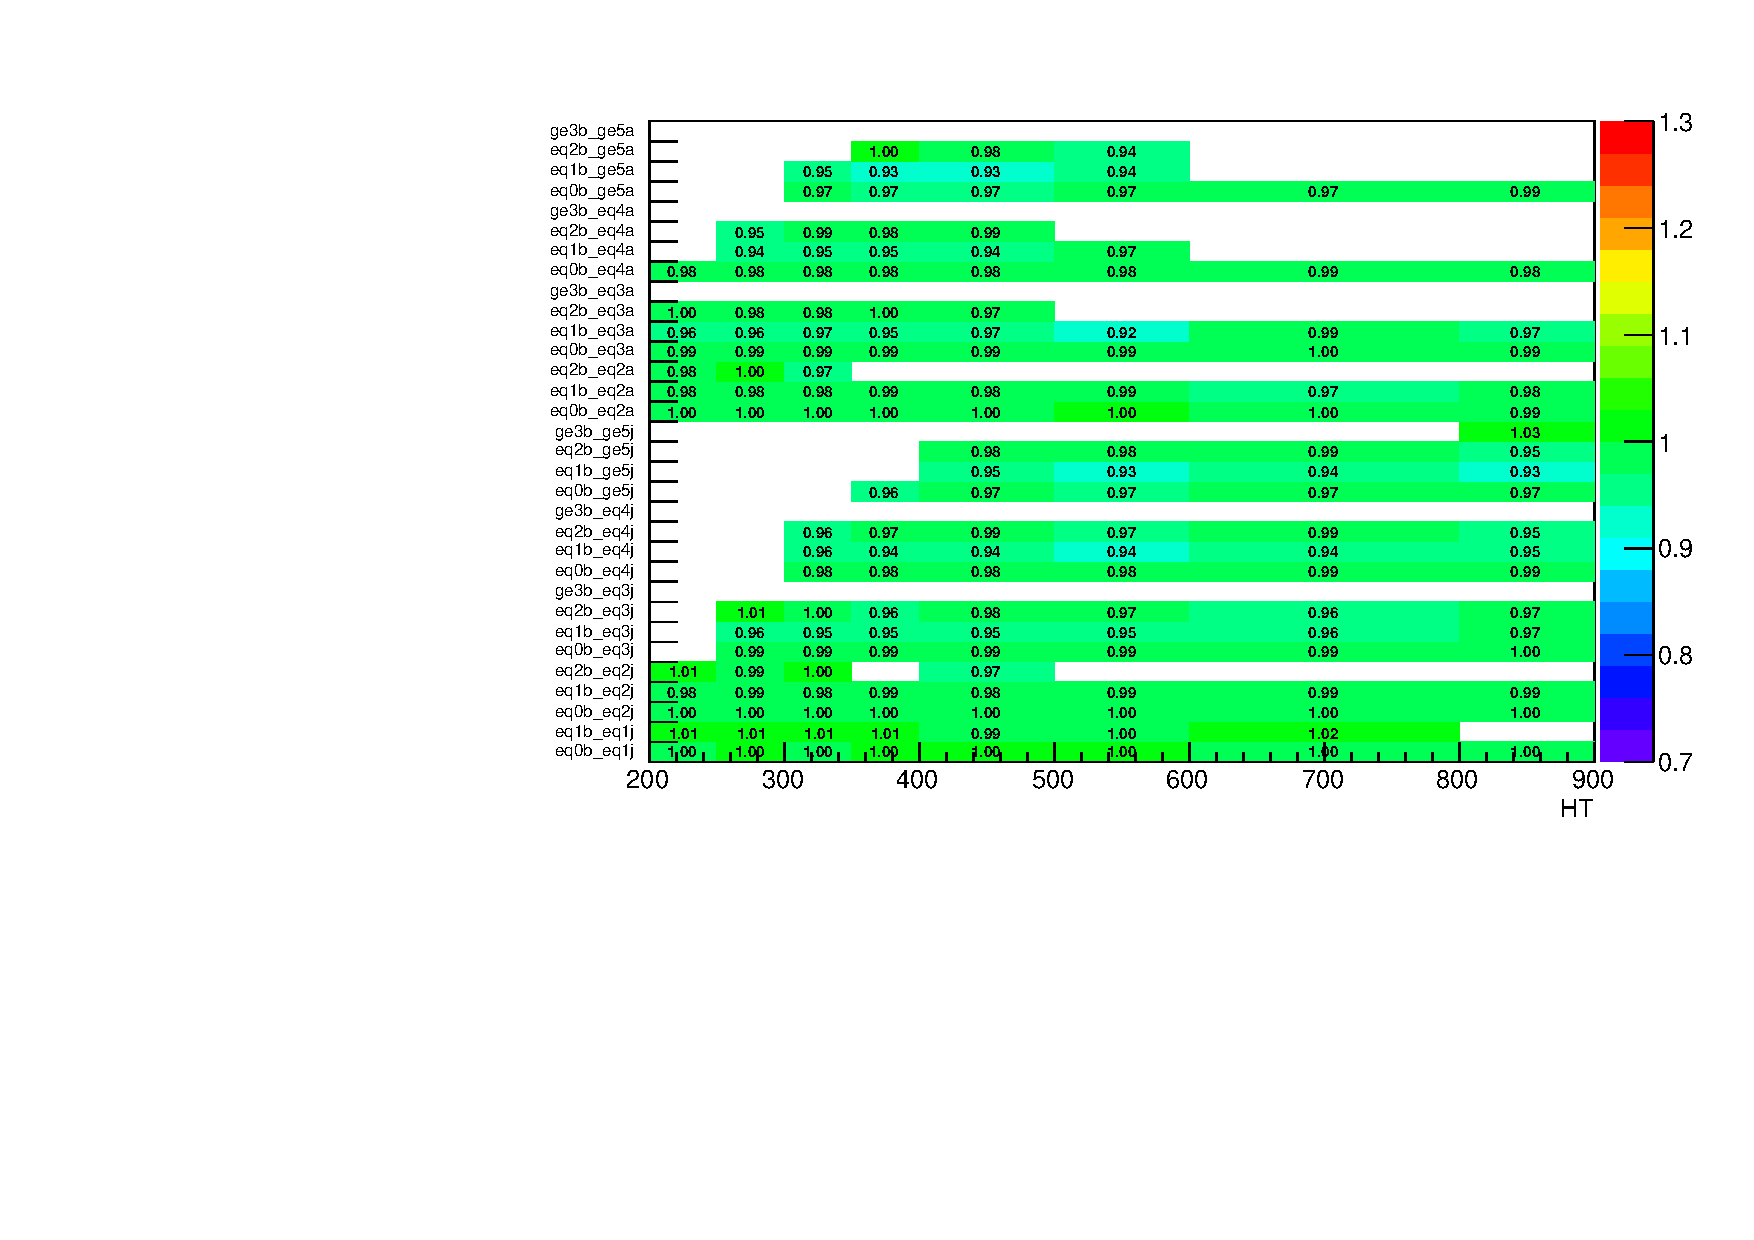
\includegraphics[width=0.5\textwidth]{figures/mcSystematics/Zinv/mu/ratiotfh_ht_mht_allbsfWeight_Down.pdf}
  }\\
  \subfigure[Pileup weights factors varied up]{
    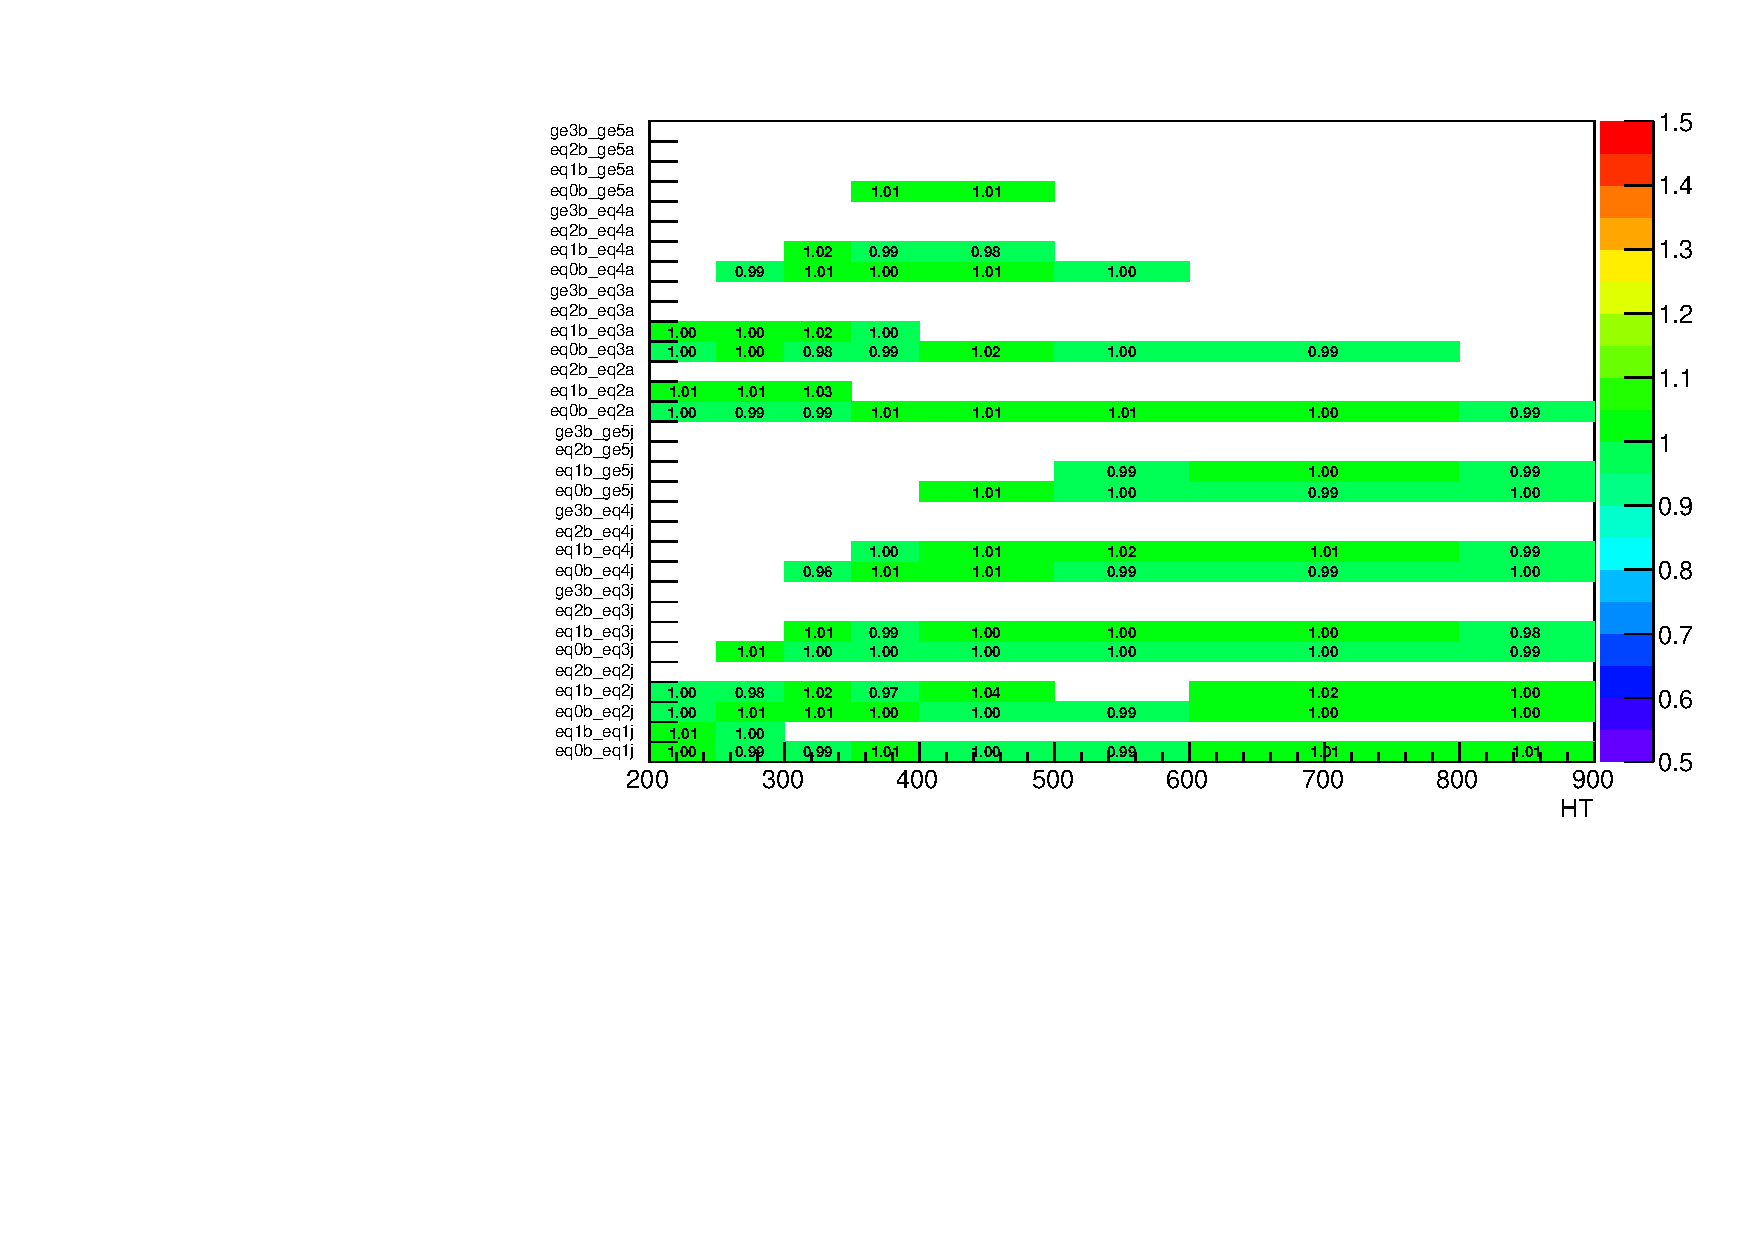
\includegraphics[width=0.5\textwidth]{figures/mcSystematics/Zinv/mu/ratiotfh_ht_mht_allpuWeight_Up.pdf}
  } ~~
  \subfigure[Pileup weights factors varied down]{
    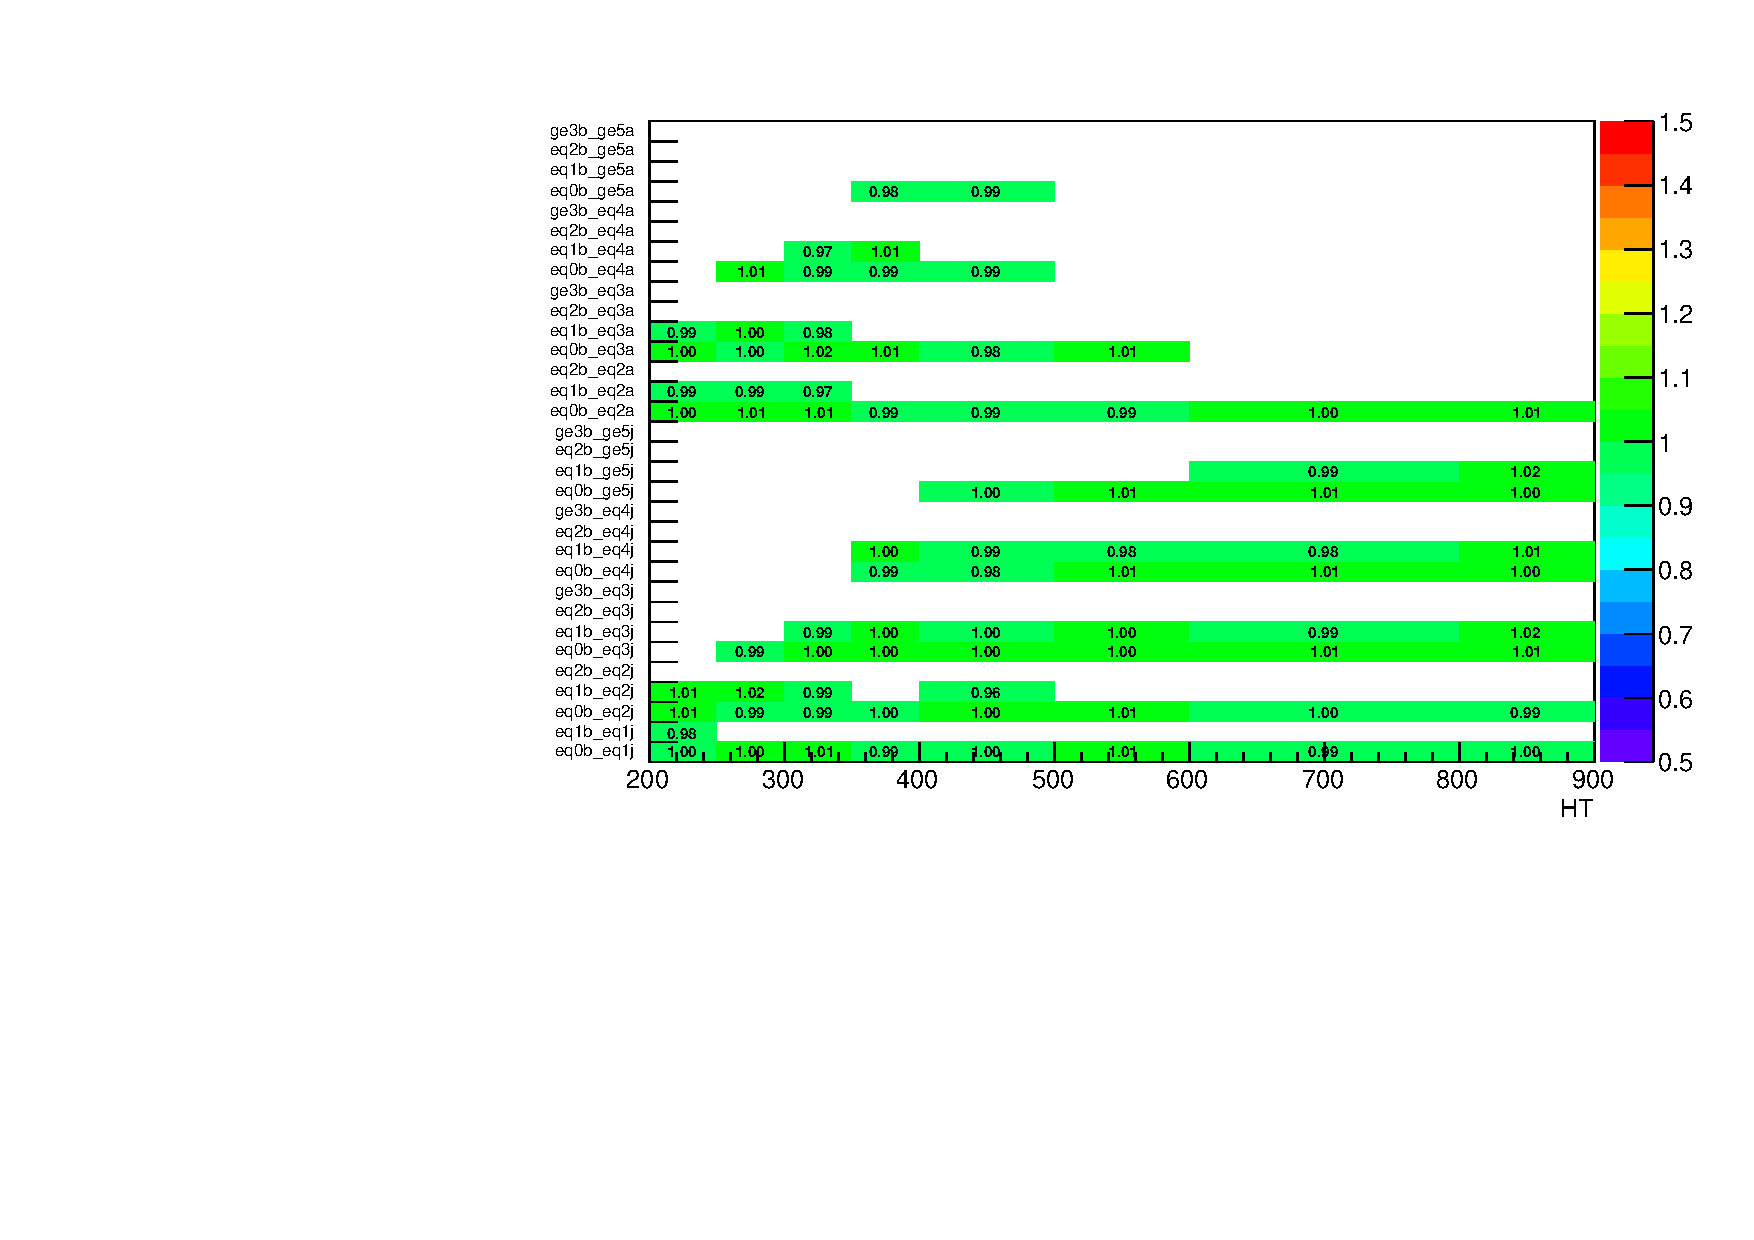
\includegraphics[width=0.5\textwidth]{figures/mcSystematics/Zinv/mu/ratiotfh_ht_mht_allpuWeight_Down.pdf}
  }\\
  \subfigure[Top $p_{T}$ weights varied up]{
    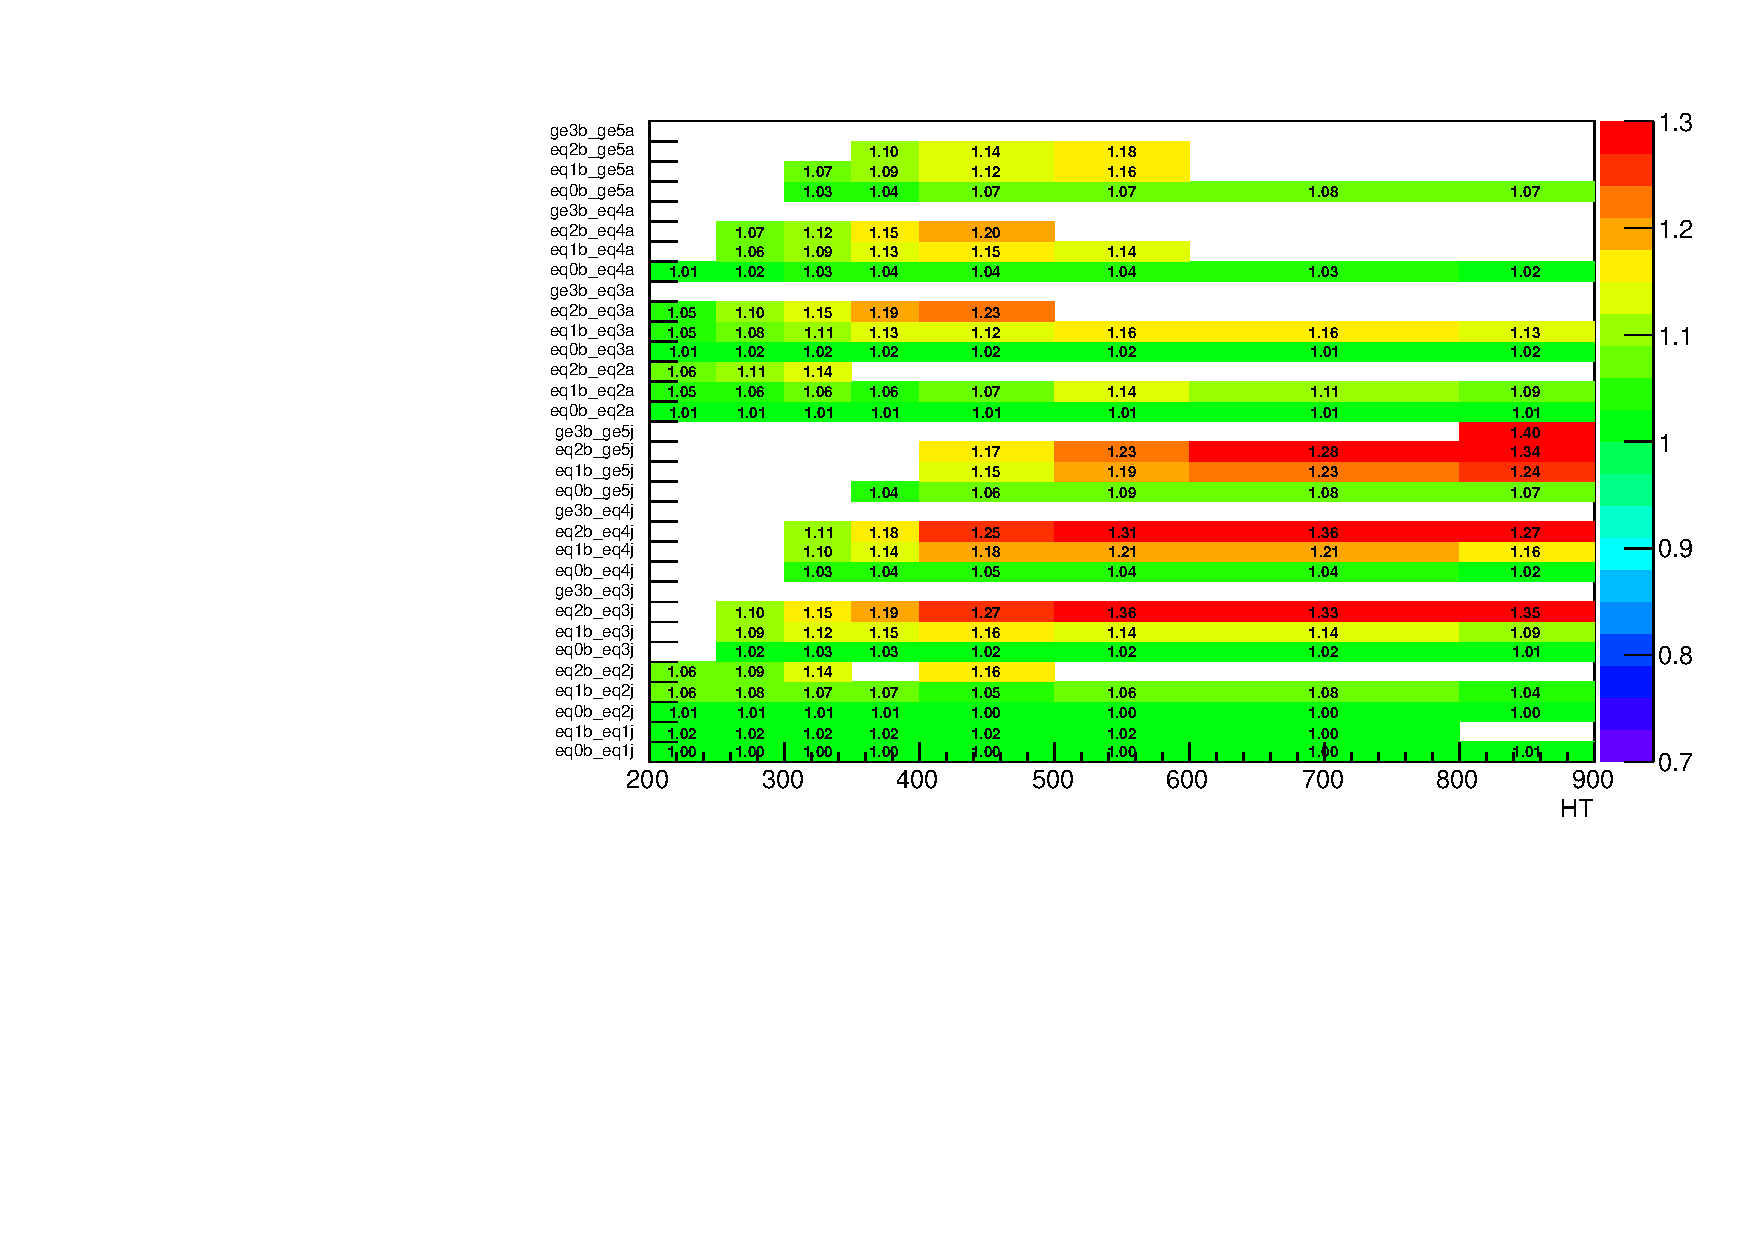
\includegraphics[width=0.5\textwidth]{figures/mcSystematics/Zinv/mu/ratiotfh_ht_mht_alltopPtWeight_Up.pdf}
  } ~~
  \subfigure[Top $p_{T}$ weights varied down]{
    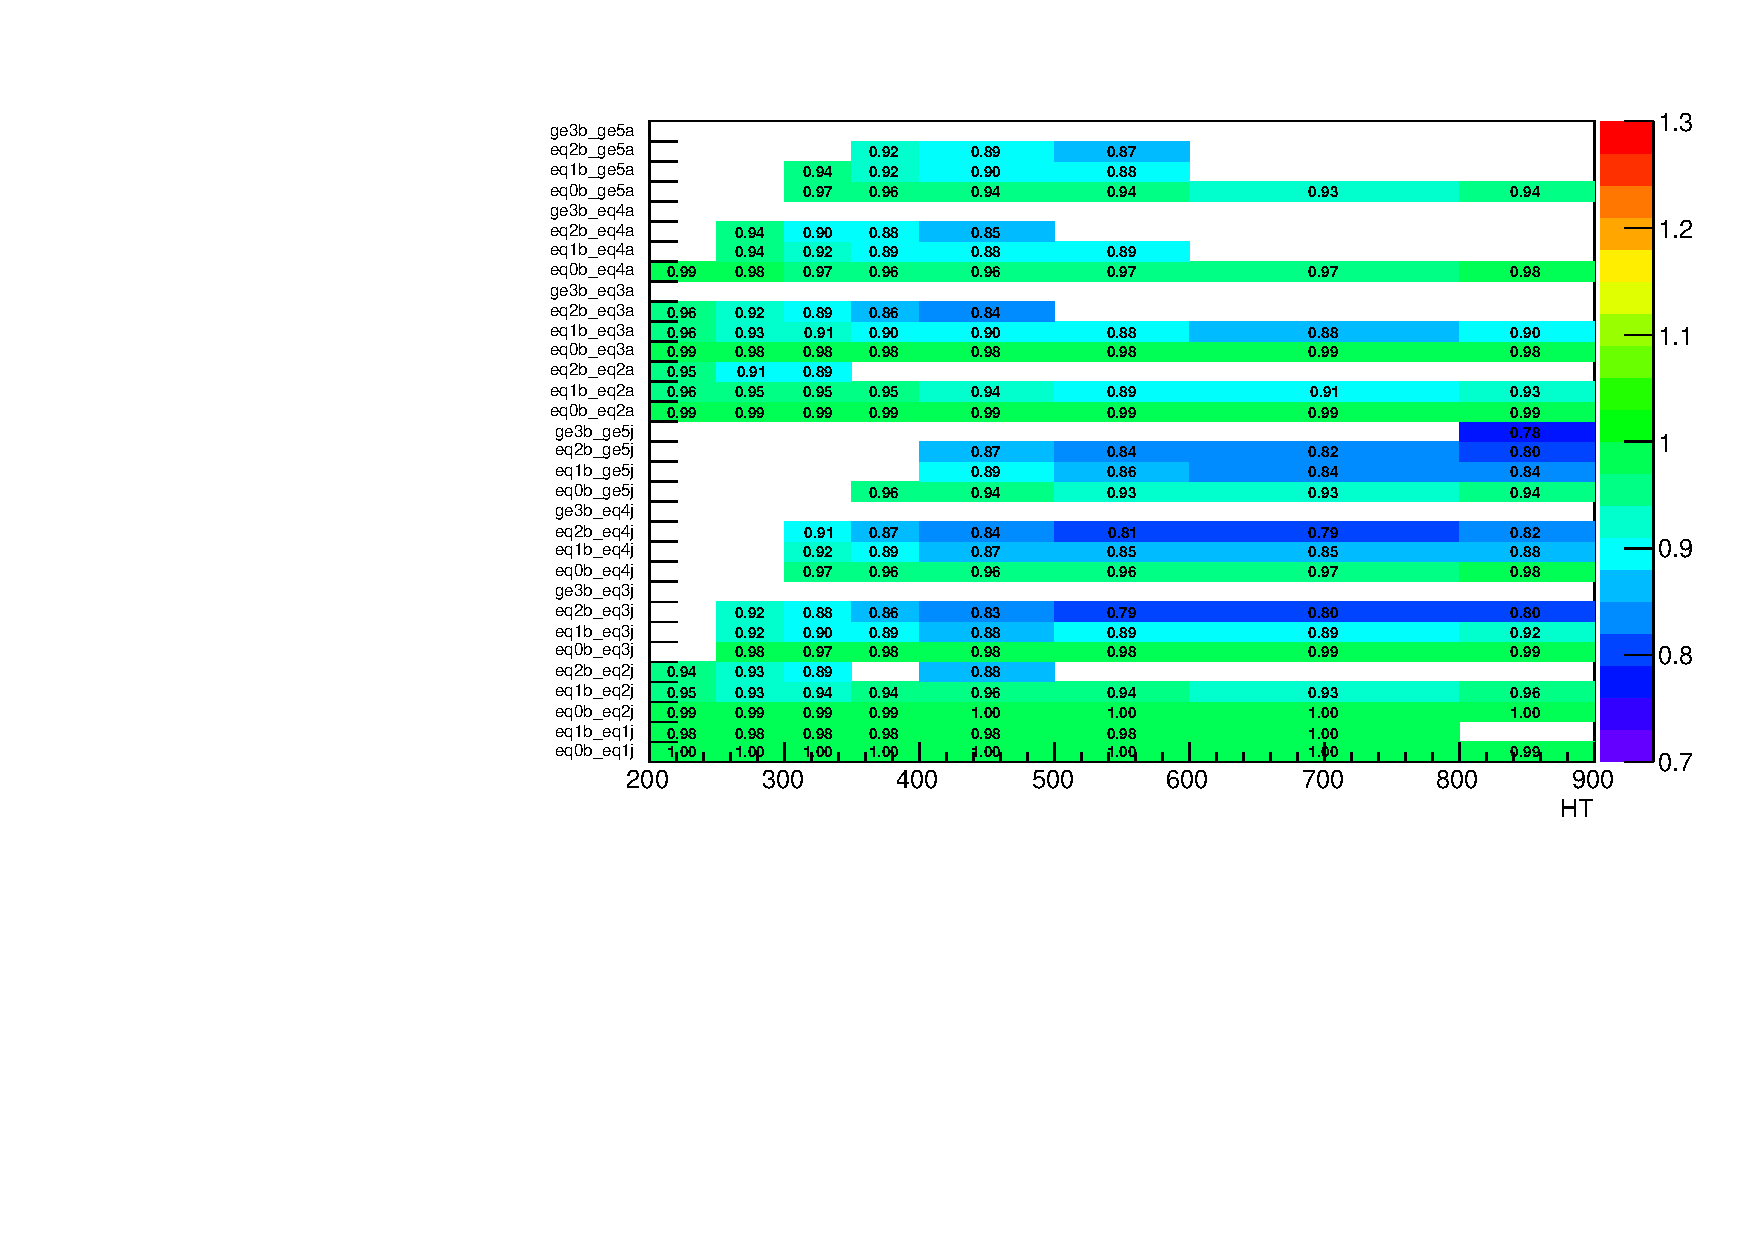
\includegraphics[width=0.5\textwidth]{figures/mcSystematics/Zinv/mu/ratiotfh_ht_mht_alltopPtWeight_Down.pdf}
  }\\
  \caption{\label{fig:muZnunuTF} The change in \mj to \znunu transfer
  factors when varying various parameters in the MC simulation by
  there upwards and downwards one sigma values. }
\end{figure}

{\bf Data-driven systematics}

To test the use of \wej and \ttbar dominated \mj events to predict the \znunu
background, $\mj \rightarrow \mmj$ closure tests are performed. These
tests also indirectly test muon acceptance effects. The results can be seen in
Fig.~\ref{fig:closureMuToMuMu}. In this test pairs of \scalht bins are
merged due to the low statistics in the \mmj control sample.

\begin{figure}[h!]
  \begin{center}
    \subfigure[]{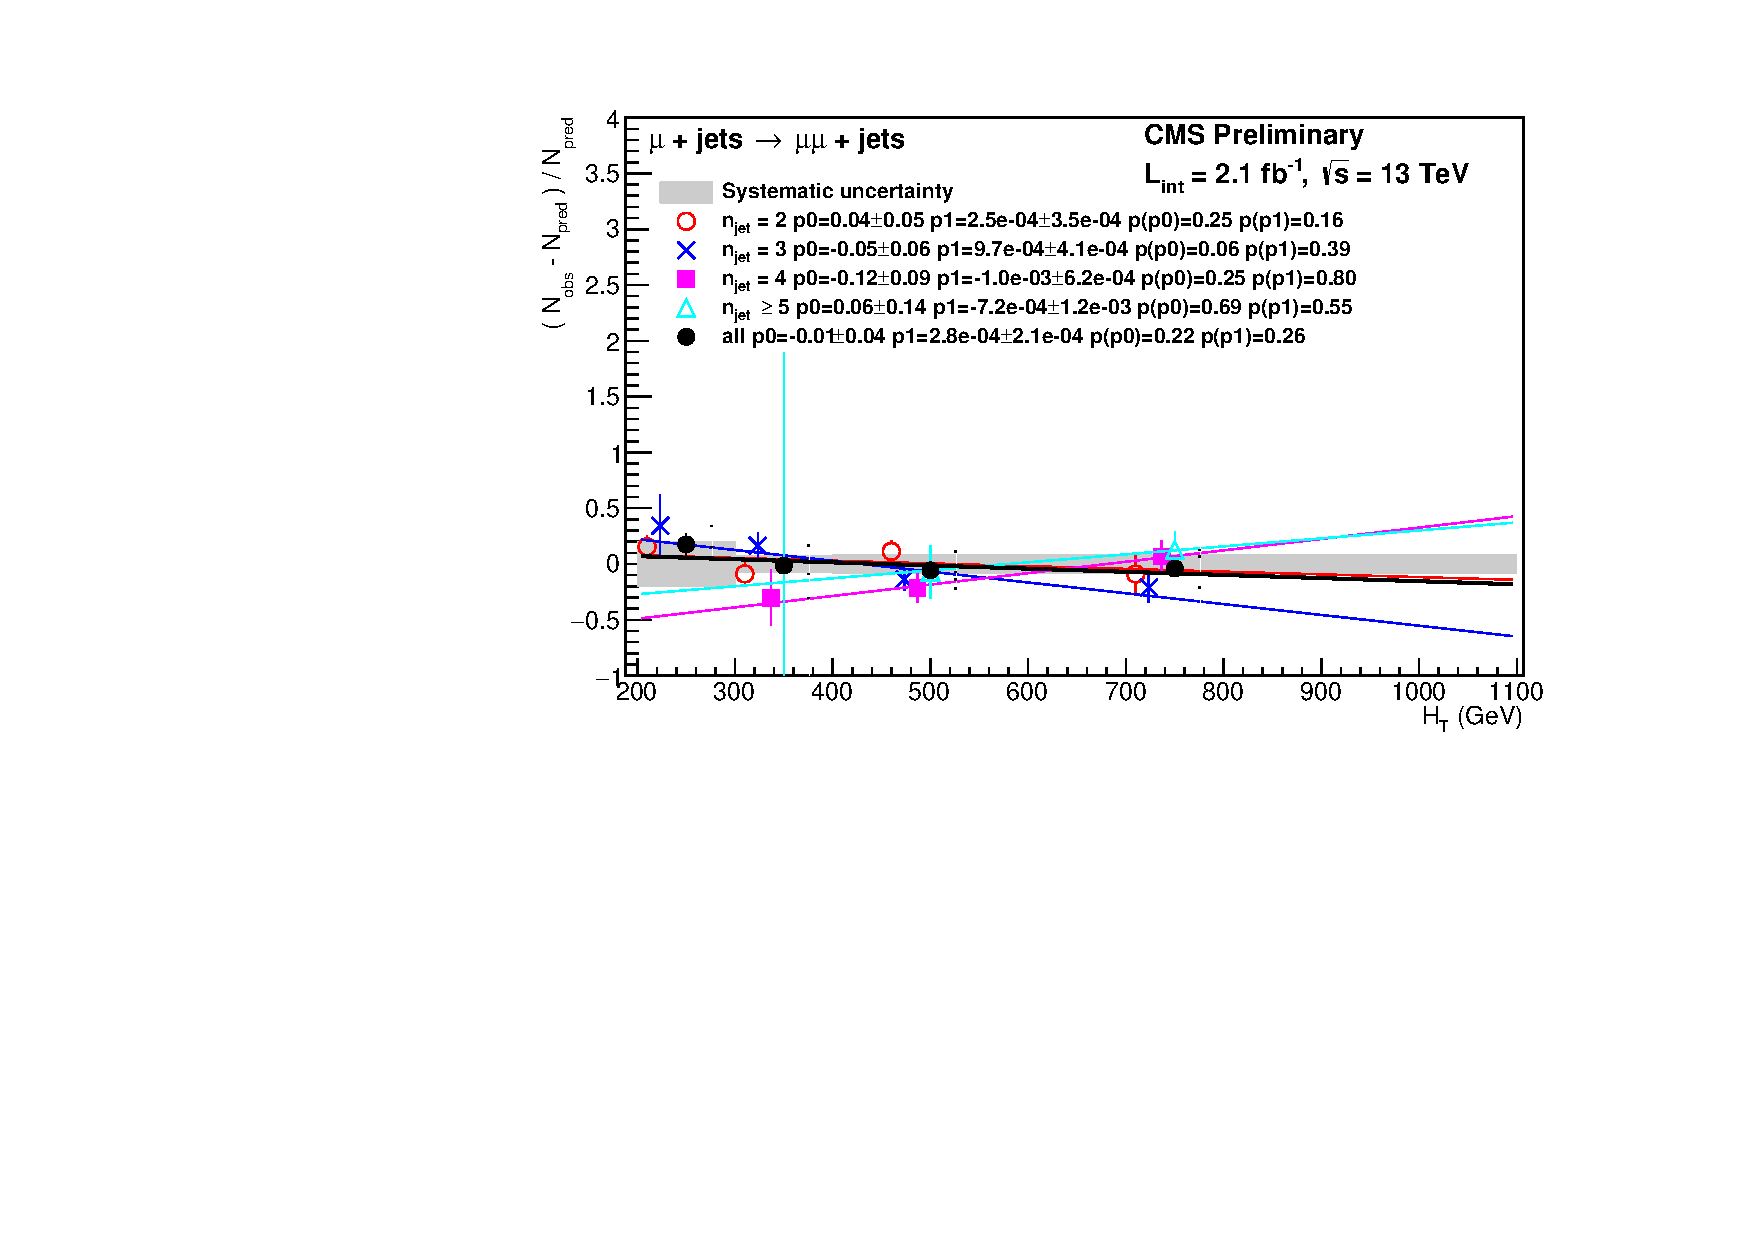
\includegraphics[width=0.45\textwidth]{figures/closureTests/mu_mumusym_half_fit.pdf}}
    ~~
    \subfigure[]{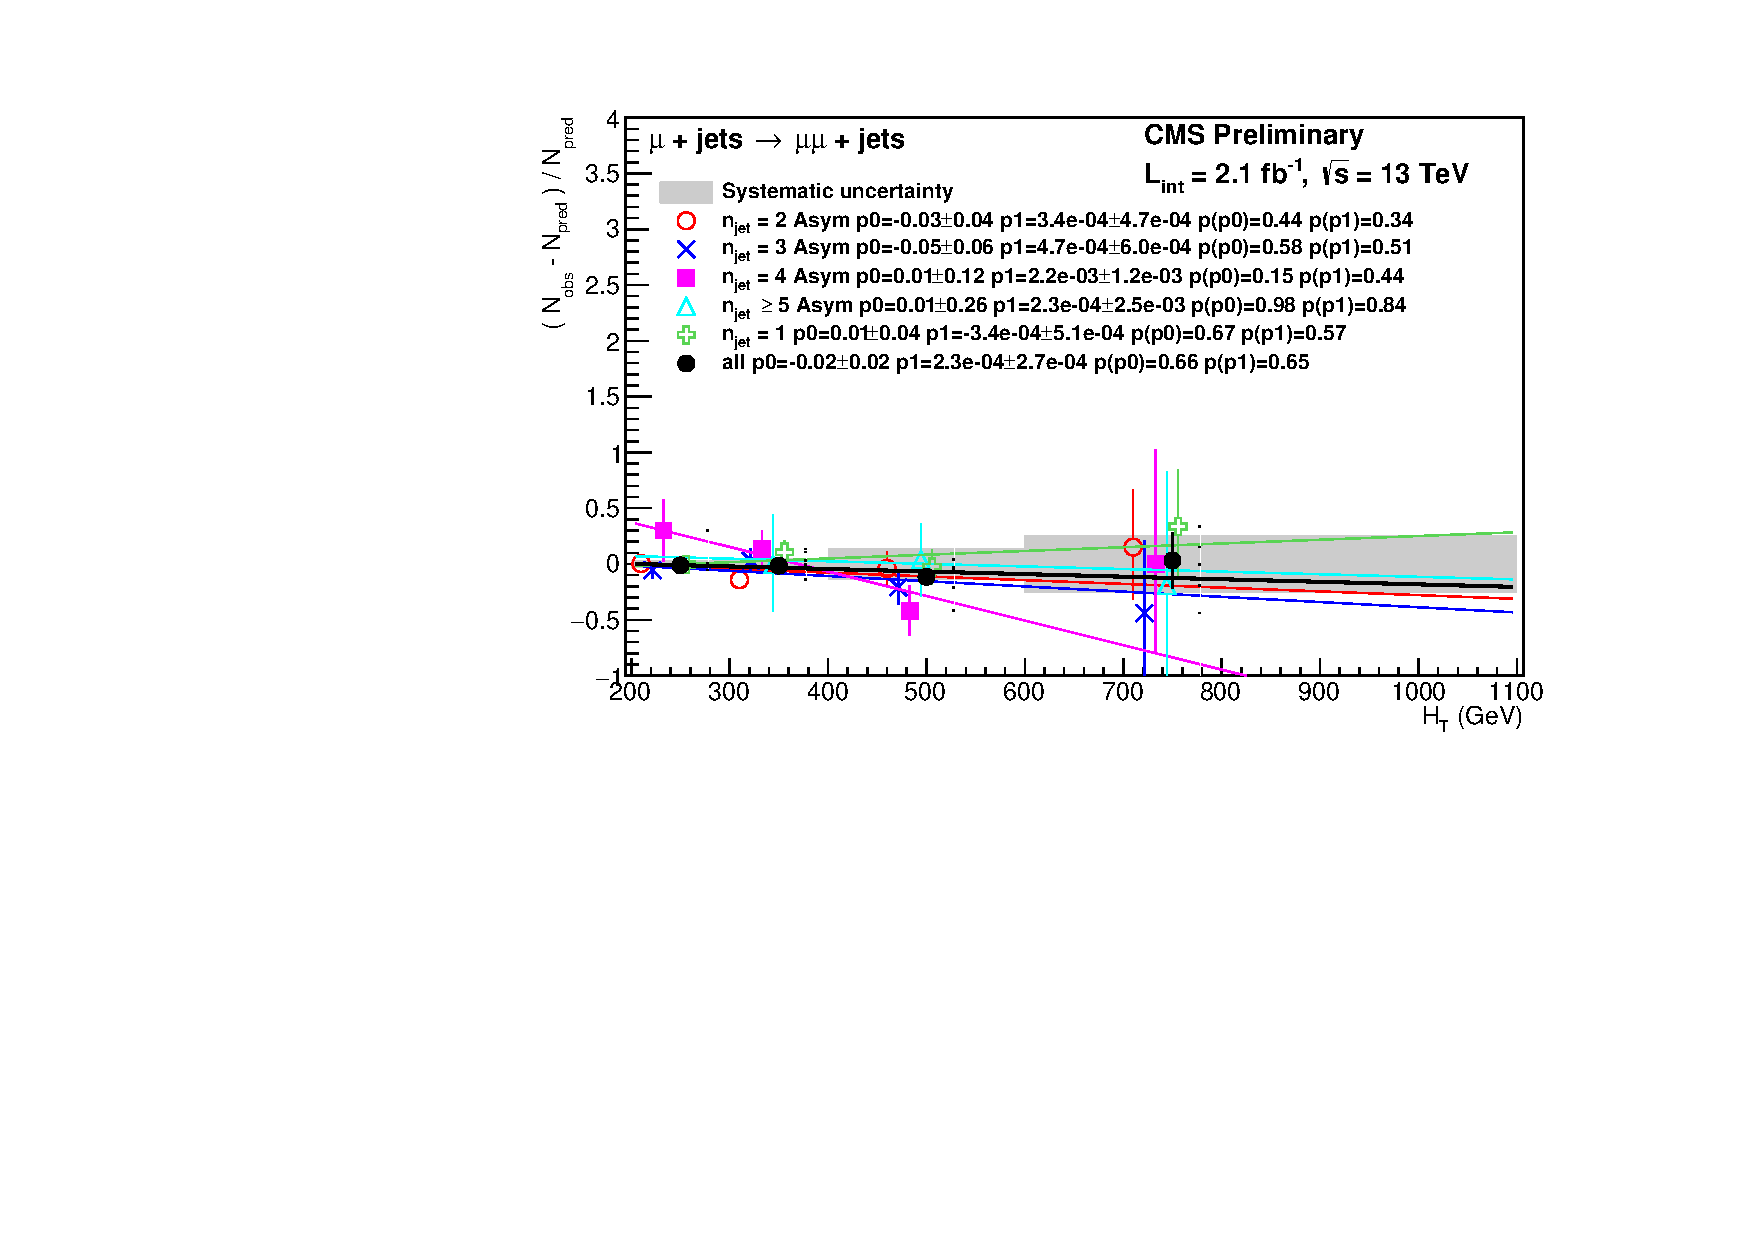
\includegraphics[width=0.45\textwidth]{figures/closureTests/mu_mumuasym_half_fit.pdf}} 
    \caption{Closure tests probing the use of the \mj control sample
      to predict the \znunu background for each
      \njet category (open symbols) overlaid on top of the systematic
      uncertainty estimates used for each of the seven \scalht bins
      (shaded bands) carried out with $2.2\ifb$ of $13\tev$
      data. The two closure tests are separated based on topology.
      Each test is fit with a linear orthogonal polynomial with the
      fit parameters on the plot.}
    \label{fig:closureMuToMuMu}
  \end{center} 
\end{figure}

Additionally, to 
test the prediction of \znunu + jets processes with
the $W$-enriched \mj control sample, we introduce the
$\mu^{+}\rightarrow\mu^{-}$ closure test, as mentioned in
Sec.~\ref{sec:backgroundmet}. The production mechanism of $W$ from pp
collisions means high $p_T$ $W$ bosons are predominantly left handed
\cite{WPol}.  For high $p_T$ bosons, this implies that $W^+$ decays to
the left handed neutrino along its direction of motion while the
lepton is pointing backward. The opposite behaviour is expected for
the $W^-$. The lepton is therefore more boosted (and the neutrino less
boosted) in $W^+$ decays than $W^-$ decays.  This leads to a larger
number of $W^+$ decays in the single lepton control regions (which
relies on the lepton $p_T$ for acceptance) than in the signal region
(which relies on the neutrino $p_T$ for acceptance). The new closure
test checks if this leads to a bias in the prediction of the \znunu +
jets background. This test can be seen in
Fig.~\ref{figclosureMuPToMuM}.

\begin{figure}[h!]
  \begin{center}
    \subfigure[]{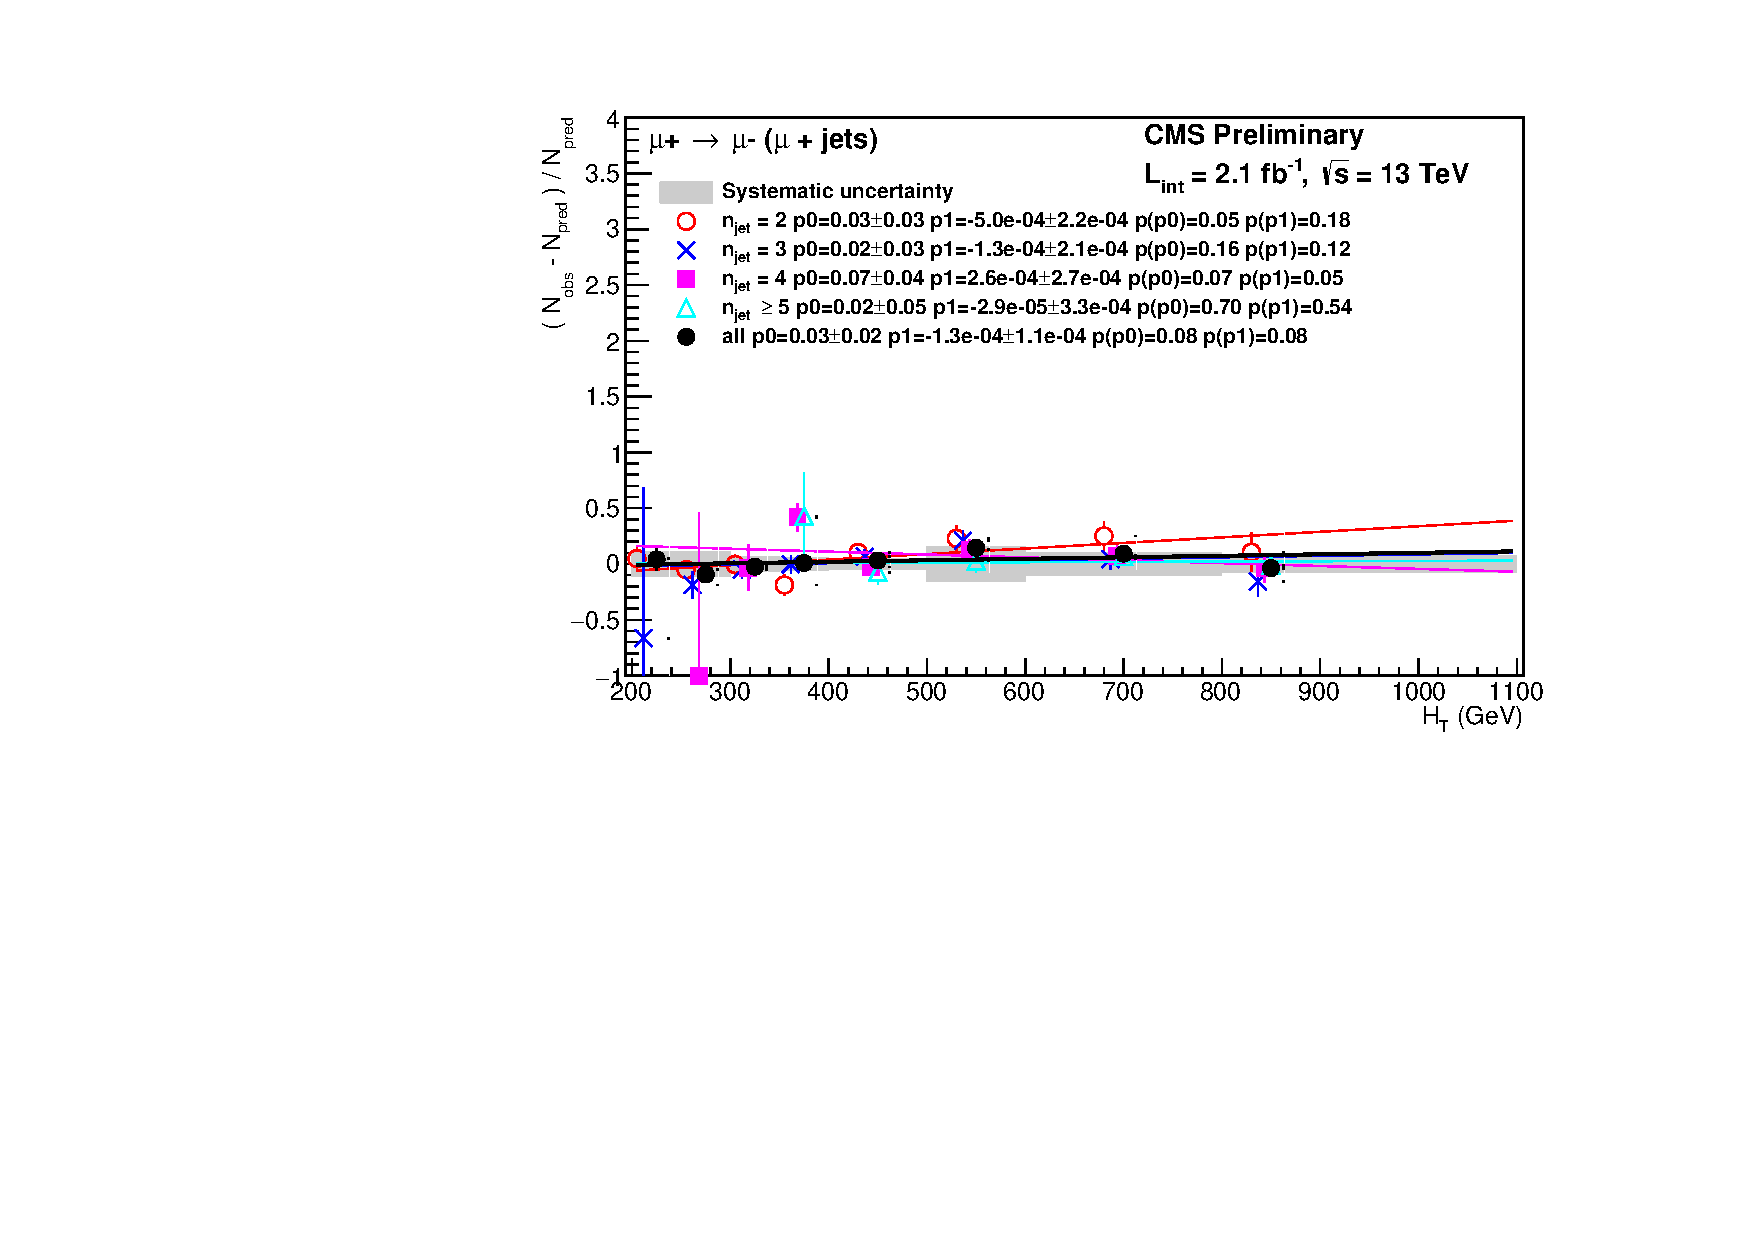
\includegraphics[width=0.45\textwidth]{figures/closureTests/muplus_muminussym__fit.pdf}}
    ~~
    \subfigure[]{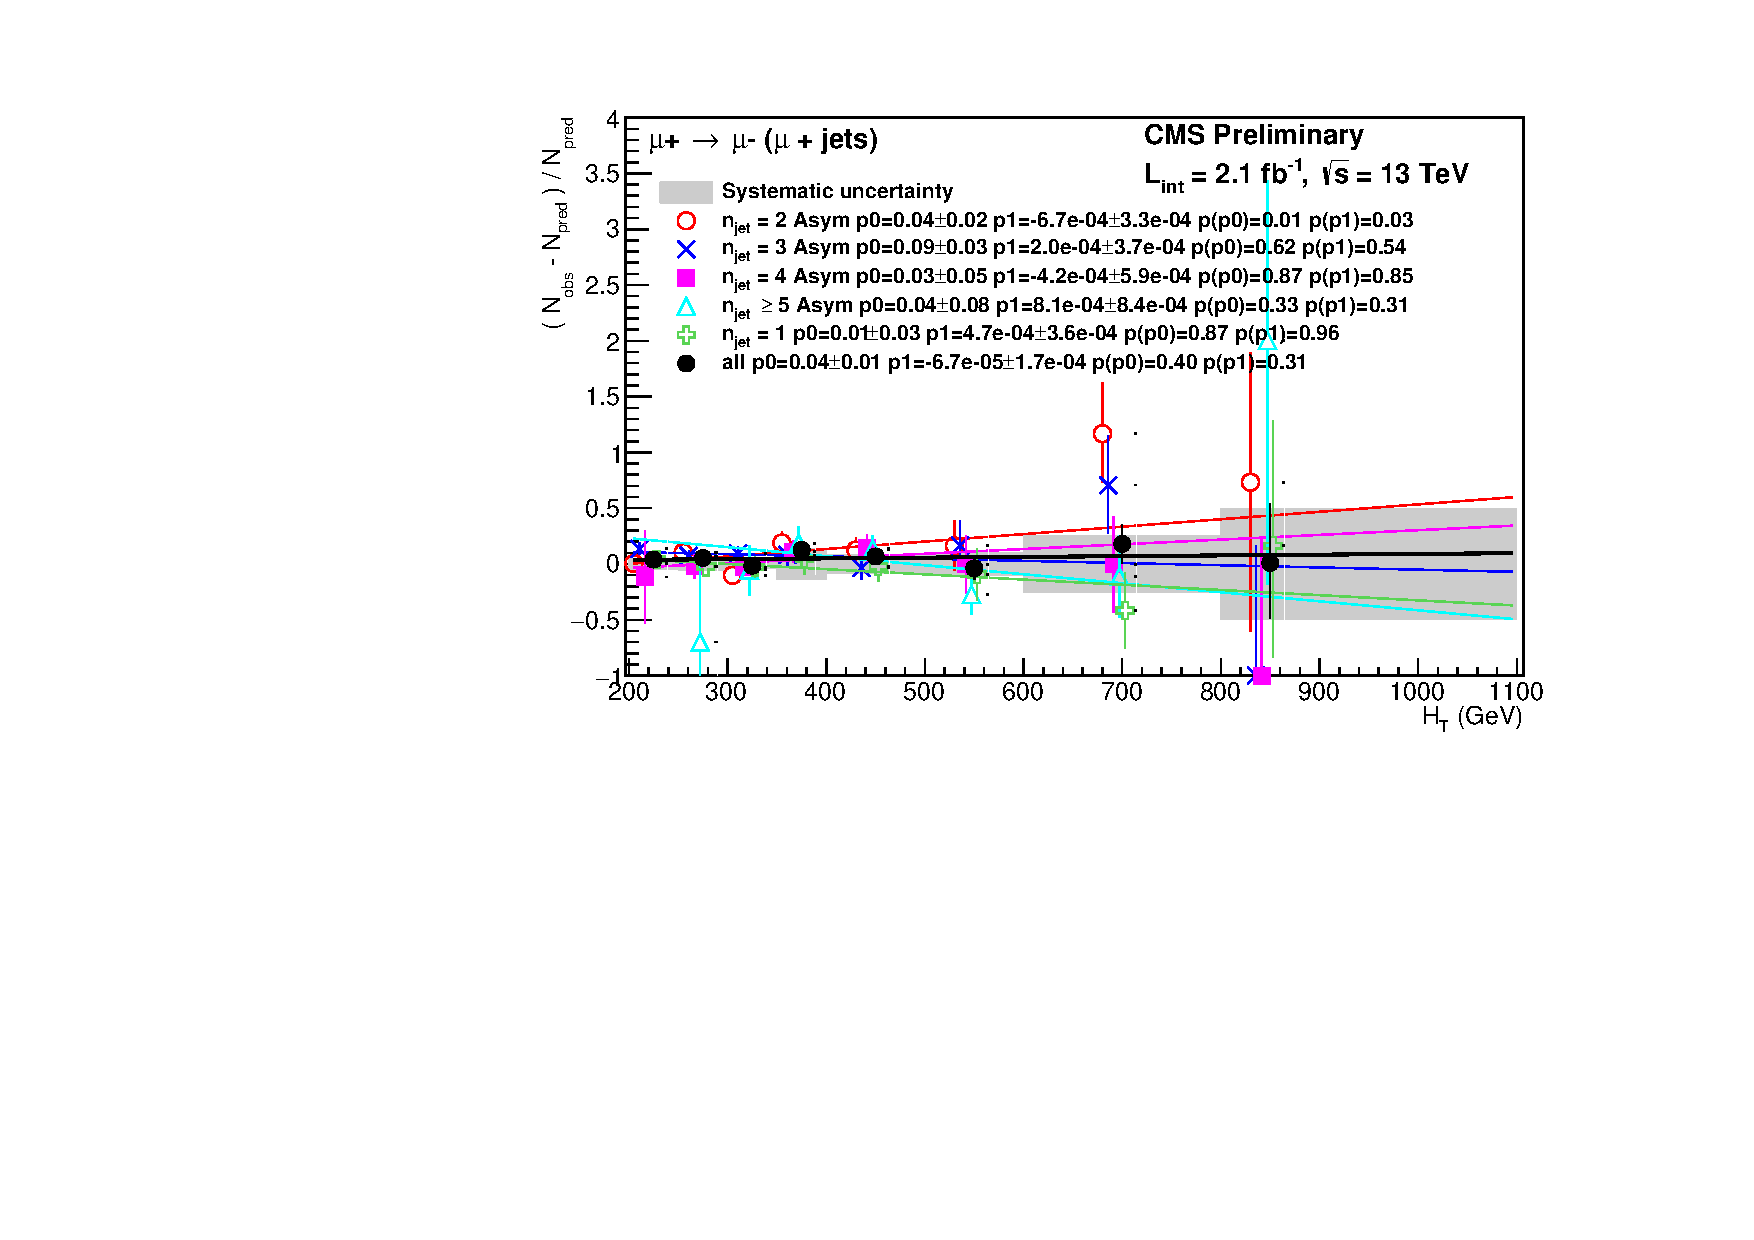
\includegraphics[width=0.45\textwidth]{figures/closureTests/muplus_muminusasym__fit.pdf}} 
    \caption{Closure tests probing the W polarisation effects that are
    relevant when using the \mj control sample for background
    prediction. These are shown for each
      \njet category (open symbols) overlaid on top of the systematic
      uncertainty estimates used for each of the seven \scalht bins
      (shaded bands) carried out with $2.2\ifb$ of $13\tev$
      data. The two closure tests are separated based on topology.
      Each test is fit with a linear orthogonal polynomial with the
      fit parameters on the plot.}
    \label{fig:closureMuPToMuM}
  \end{center} 
\end{figure}

The modelling of the \alphat and
\bdphi extrapolations are also tested with dedicated closure tests. In both
cases, it is checked that events with genuine \met found in the core
of the variable distribution below some threshold value can be used to
predict the events in the tail (above the same threshold value). The
contribution to the systematic error for \met extrapolation is taken
from the \alphat closure tests for bins with $\scalht<800\gev$ and
the \bdphi tests for bins with $\scalht>800\gev$.

The closure tests in Fig.~\ref{fig:closureAlphaT} probe the modelling
of the \alphat distribution (following the application of the $\mht >
130\gev$ requirement in the control and signal regions) in genuine
\met events as a function of \scalht. This is important to verify the
approach of using \mj and \mmj samples without an \alphat requirement
to make background predictions in the signal region. The tests
confront data yields in a \mj  samples with an \alphat
requirement against predictions determined in a \mj sample with
the \alphat requirement inverted. As usual, corresponding expectations
from simulation are obtained to construct the transfer factors
required to make the predictions.

\begin{figure}[h!]
  \begin{center}
    \subfigure[]{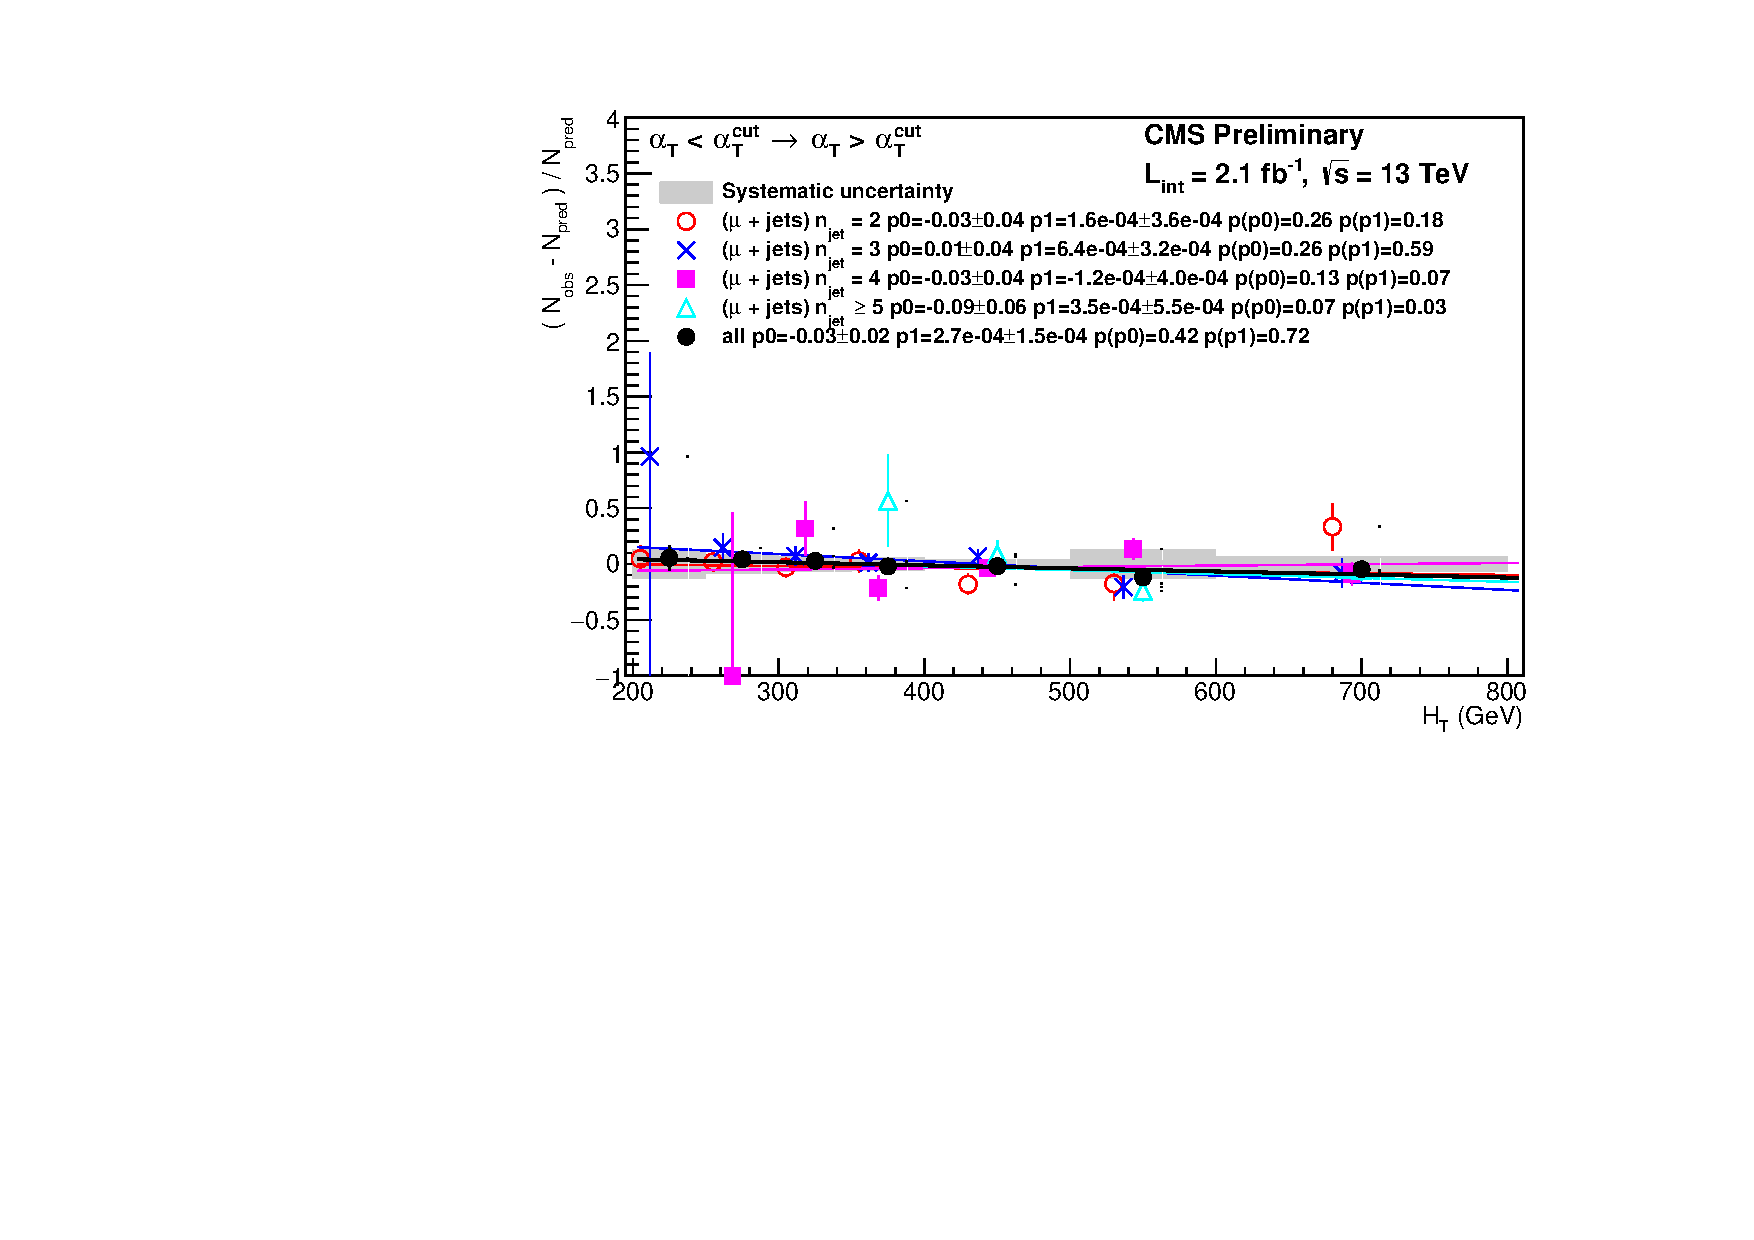
\includegraphics[width=0.45\textwidth]{figures/closureTests/alphaTsym__fit.pdf}}
    ~~
    \subfigure[]{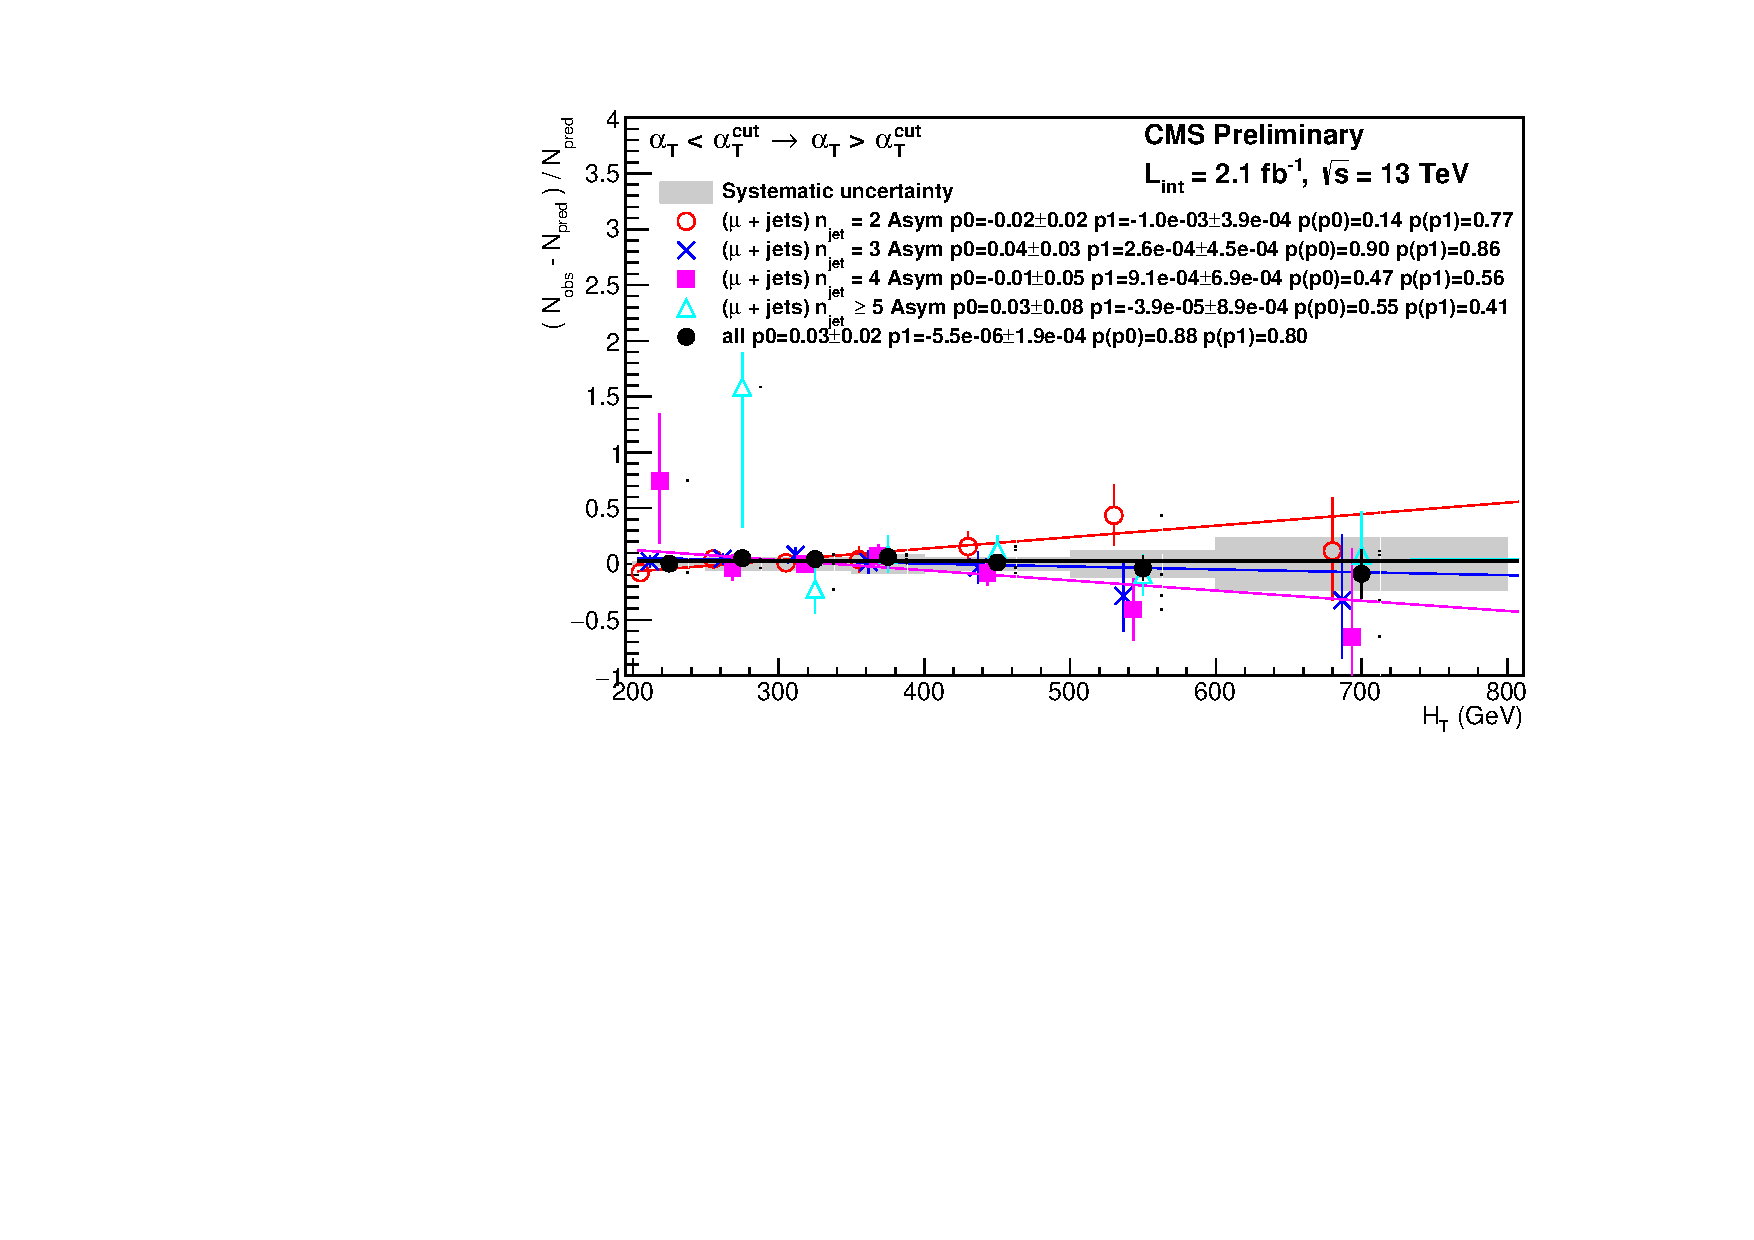
\includegraphics[width=0.45\textwidth]{figures/closureTests/alphaTasym__fit.pdf}} 
    \caption{Closure tests probing the \alphat extrapolation for each
      \njet category (open symbols) overlaid on top of the systematic
      uncertainty estimates used for each of the seven \scalht bins
      (shaded bands) carried out with $2.2\ifb$ of $13\tev$
      data. The two closure tests are separated based on topology.
      Each test is fit with a linear orthogonal polynomial with the
      fit parameters on the plot.}
    \label{fig:closureAlphaT}
  \end{center} 
\end{figure}

% \begin{table}[h!]
%   \caption{Systematic uncertainties (percent) in the
%     predictions of the $\ttbar$W and $\znunu$ (the latter in
%     parentheses) background components as a function of \scalht due to
%     the extrapolation in the \alphat (\bdphi) variable in the region
%     $\scalht > 800\gev$ ($\scalht > 800\gev$), as determined from
%     ensembles of closure tests in multiple data control samples. The
%     data control samples correspond to an integrated luminosity of
%     2.1\fbinv.} 
%   \label{tab:alphaTSyst}
%   \centering
%   \footnotesize
%   \begin{tabular}{ cccccccc }
%     \hline
%     \hline
%     \multicolumn{8}{c}{\scalht bin (GeV)}                                       \\
%     \hline
%     200   & 250     & 300     & 350     & 400     & 500     & 600     & 800     \\
%     10 (10) & 7 (7) & 8 (8) & 17 (17) & 14 (14) & 24 (24) & 27 (27) & 22 (22) \\
%     \hline
%     \hline
%   \end{tabular}
% \end{table}

The closure tests in Fig.~\ref{fig:closureBDPhi} probe the modelling
of the $\Delta\phi *$ distribution in genuine \met events as a
function of \scalht. This is important to verify the approach of using
\mj and \mmj samples without an $\Delta\phi *$ requirement to make
background predictions in the signal region. The tests confront data
yields in a \mj (\mmj) samples with an $\Delta\phi *$ requirement
against predictions determined in a \mj (\mmj) sample with the
$\Delta\phi *$ requirement inverted. 

\begin{figure}[h!]
  \begin{center}
    \subfigure[]{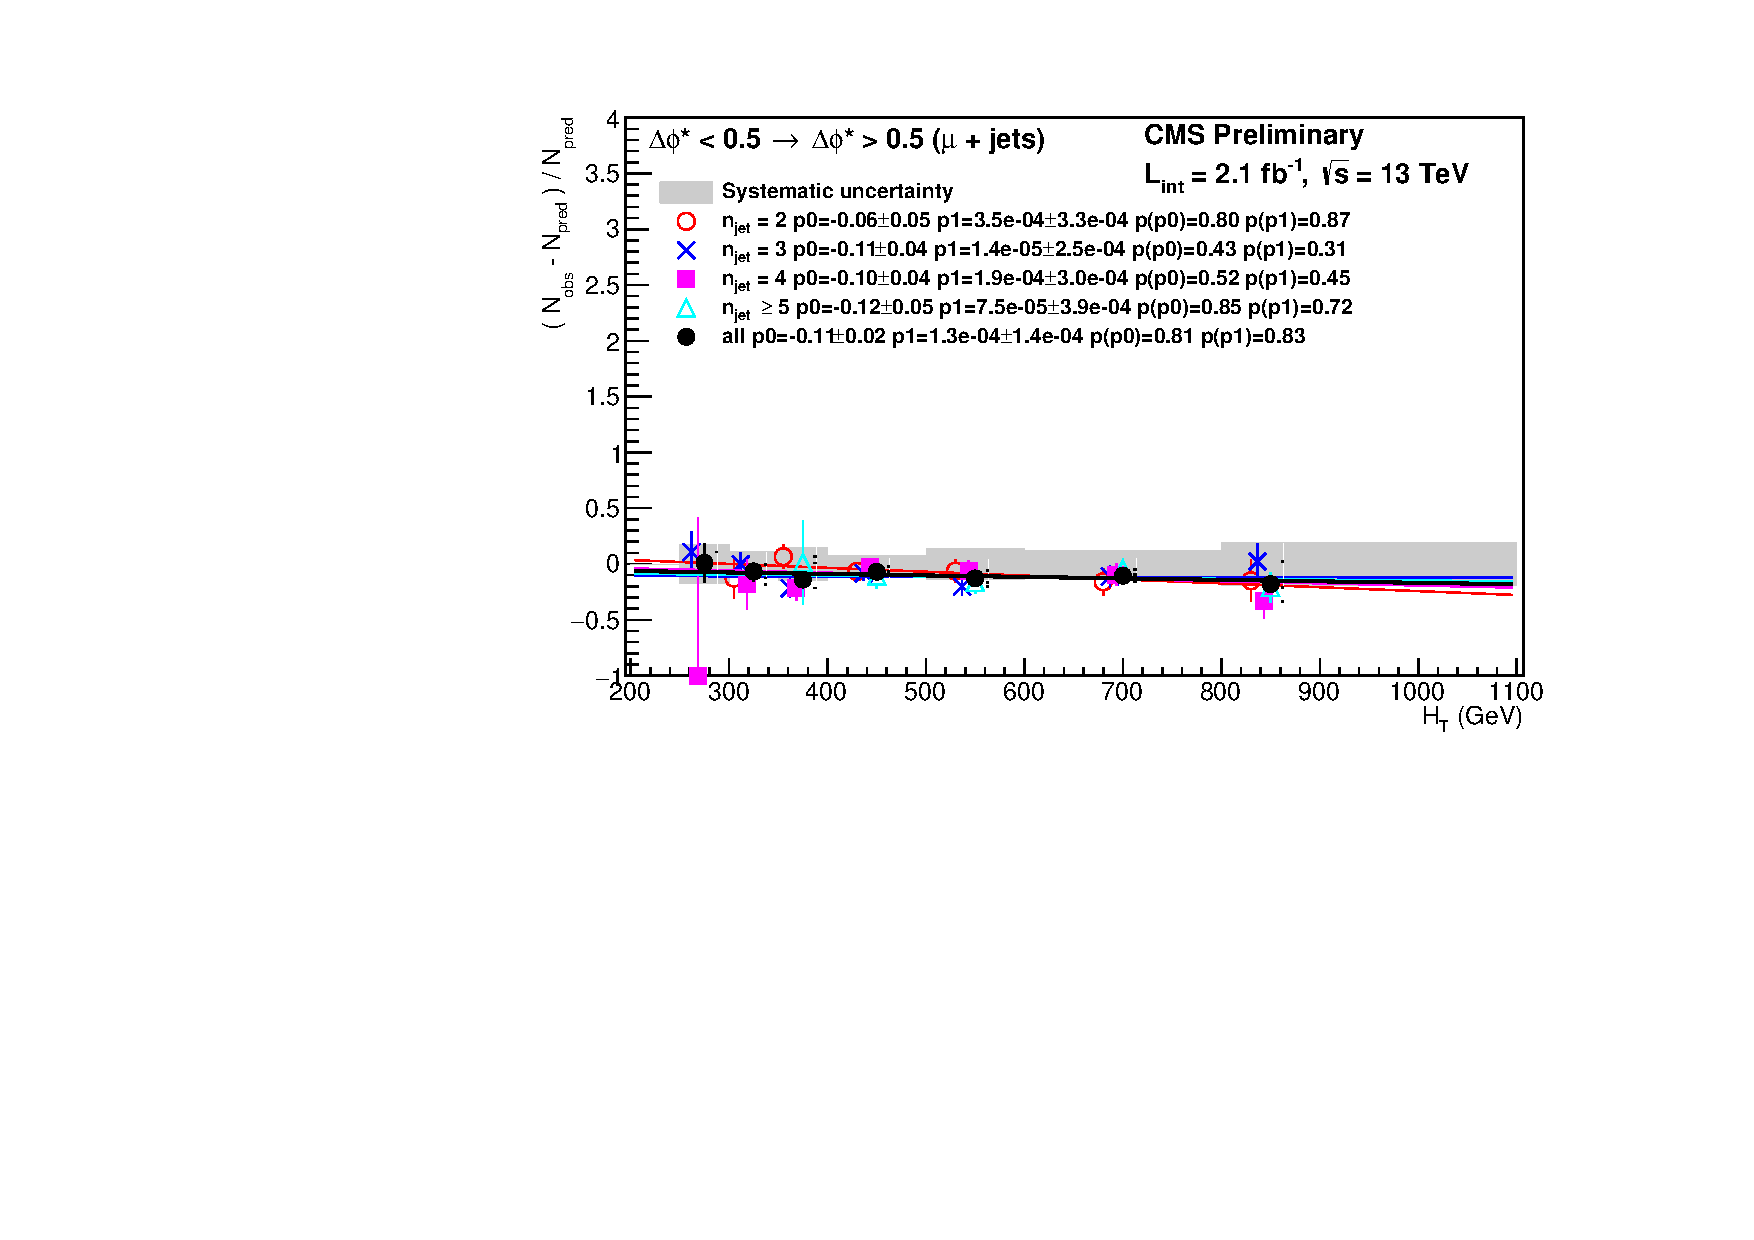
\includegraphics[width=0.45\textwidth]{figures/closureTests/bDPhisym__fit.pdf}}
    ~~
    \subfigure[]{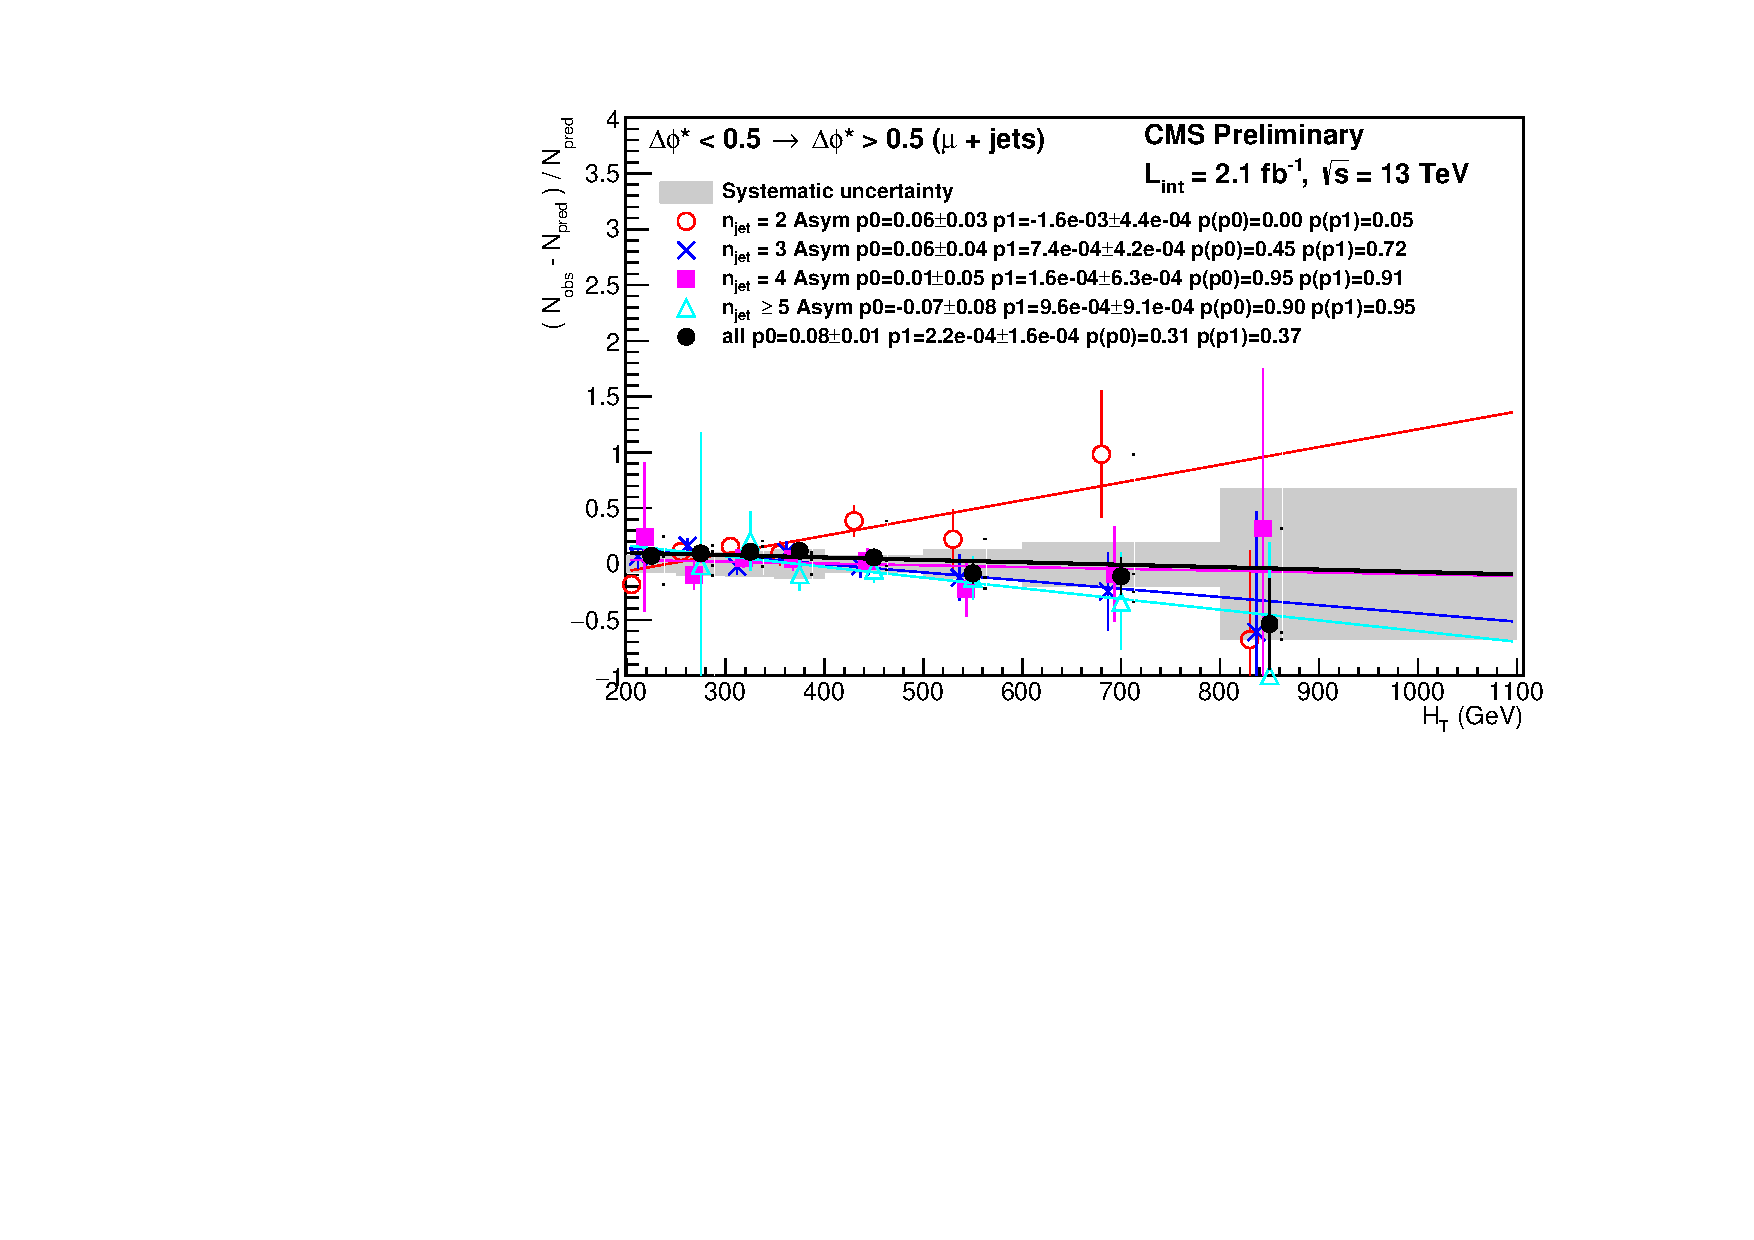
\includegraphics[width=0.45\textwidth]{figures/closureTests/bDPhiasym__fit.pdf}} 
    \caption{Closure tests probing the \bdphi extrapolation for each
      \njet category (open symbols) overlaid on top of the systematic
      uncertainty estimates used for each of the seven \scalht bins
      (shaded bands) carried out with $2.2\ifb$ of $13\tev$
      data. The two closure tests are separated based on topology.
      Each test is fit with a linear orthogonal polynomial with the
      fit parameters on the plot.}
    \label{fig:closureBDPhi}
  \end{center} 
\end{figure}

\subsubsection{Uncertainties the prediction of the \znunu
background with the \mmj control sample}

{\bf Variations on the transfer factors from simulation}

All the MC variations described in Sec~\ref{sec:mc-systematics} are
carried out for the transfer factors from the \mmj control region to
the \znunu background prediction. The results are shown in
Fig.~\ref{mumuZnunuTF}.

\begin{figure}[]
  \centering
  \subfigure[Jet energy scale varied up]{
    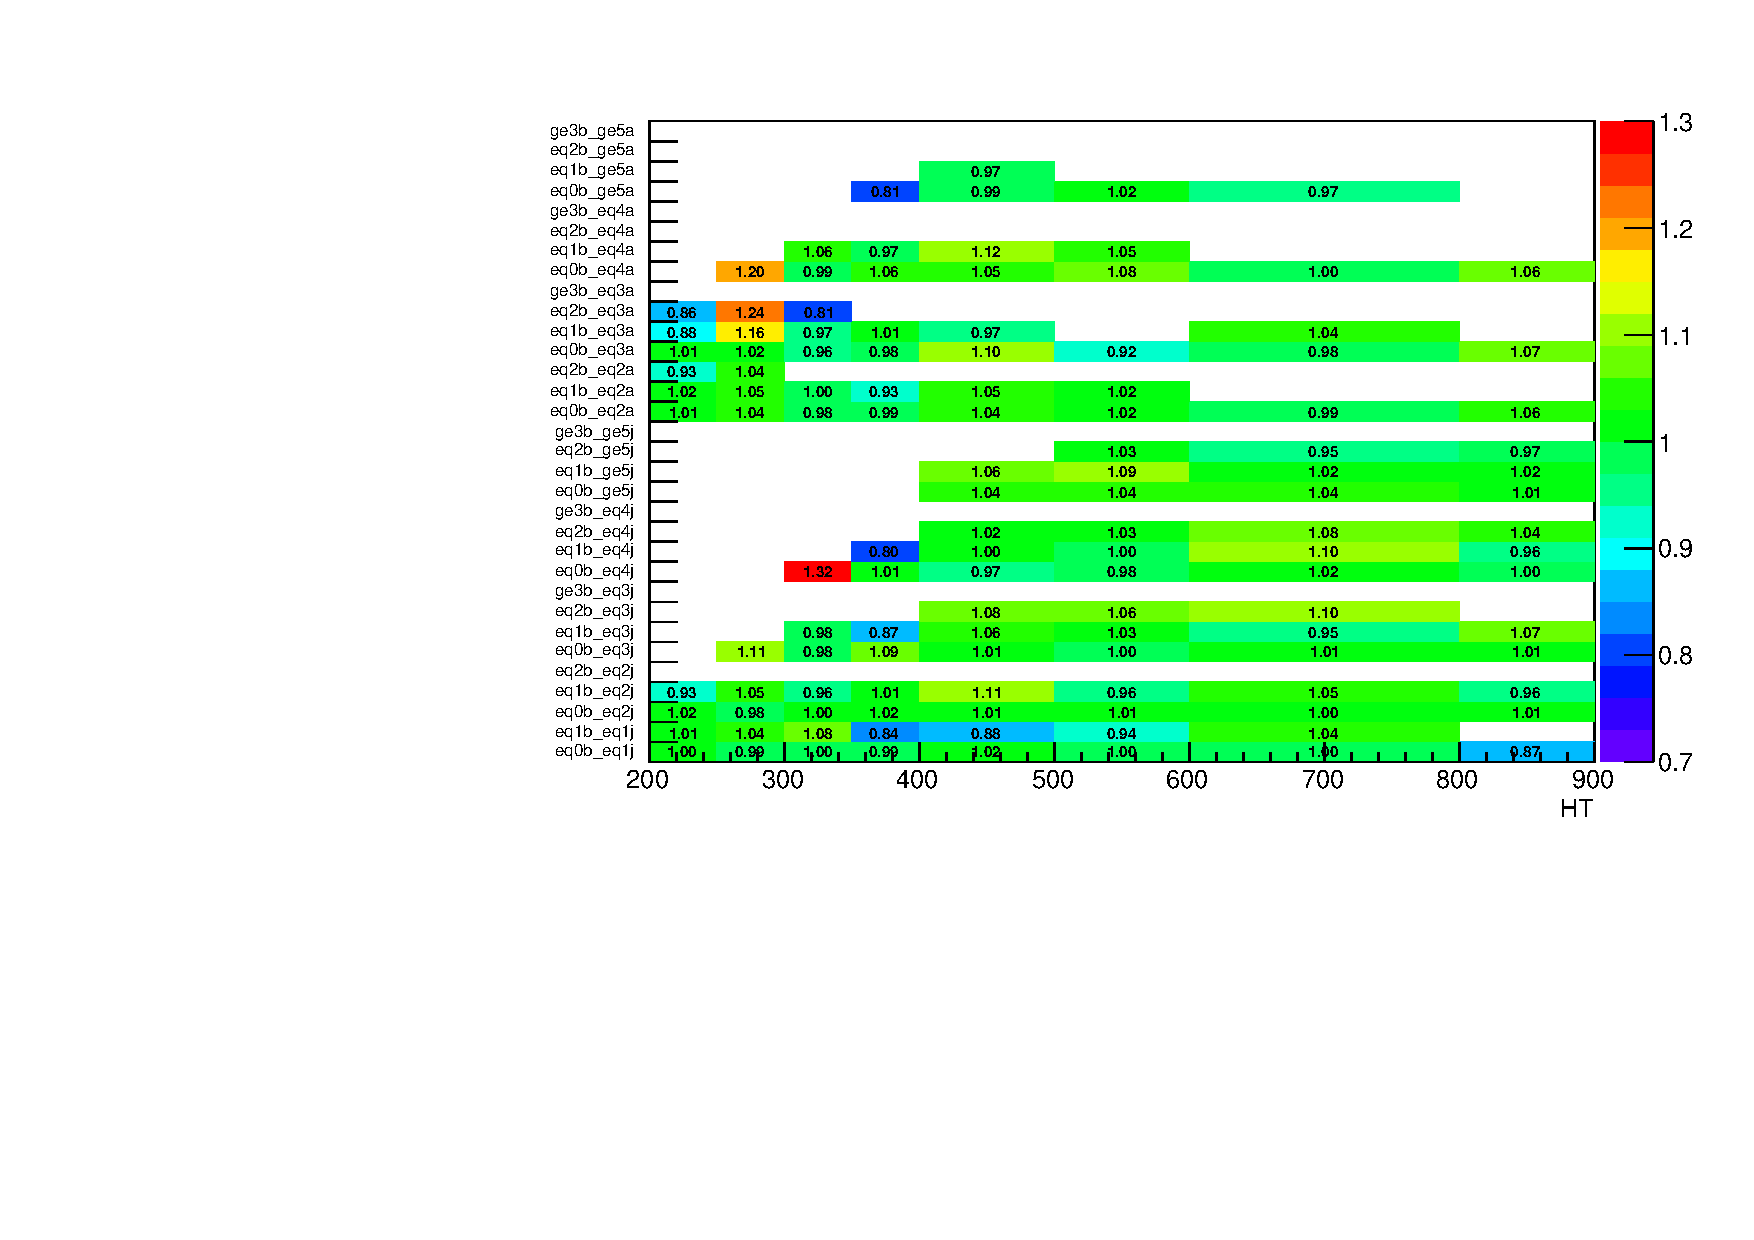
\includegraphics[width=0.5\textwidth]{figures/mcSystematics/Zinv/mumu/ratiotfh_ht_mht_alljecWeight_Up.pdf}
  } ~~
  \subfigure[Jet energy scale varied down]{
    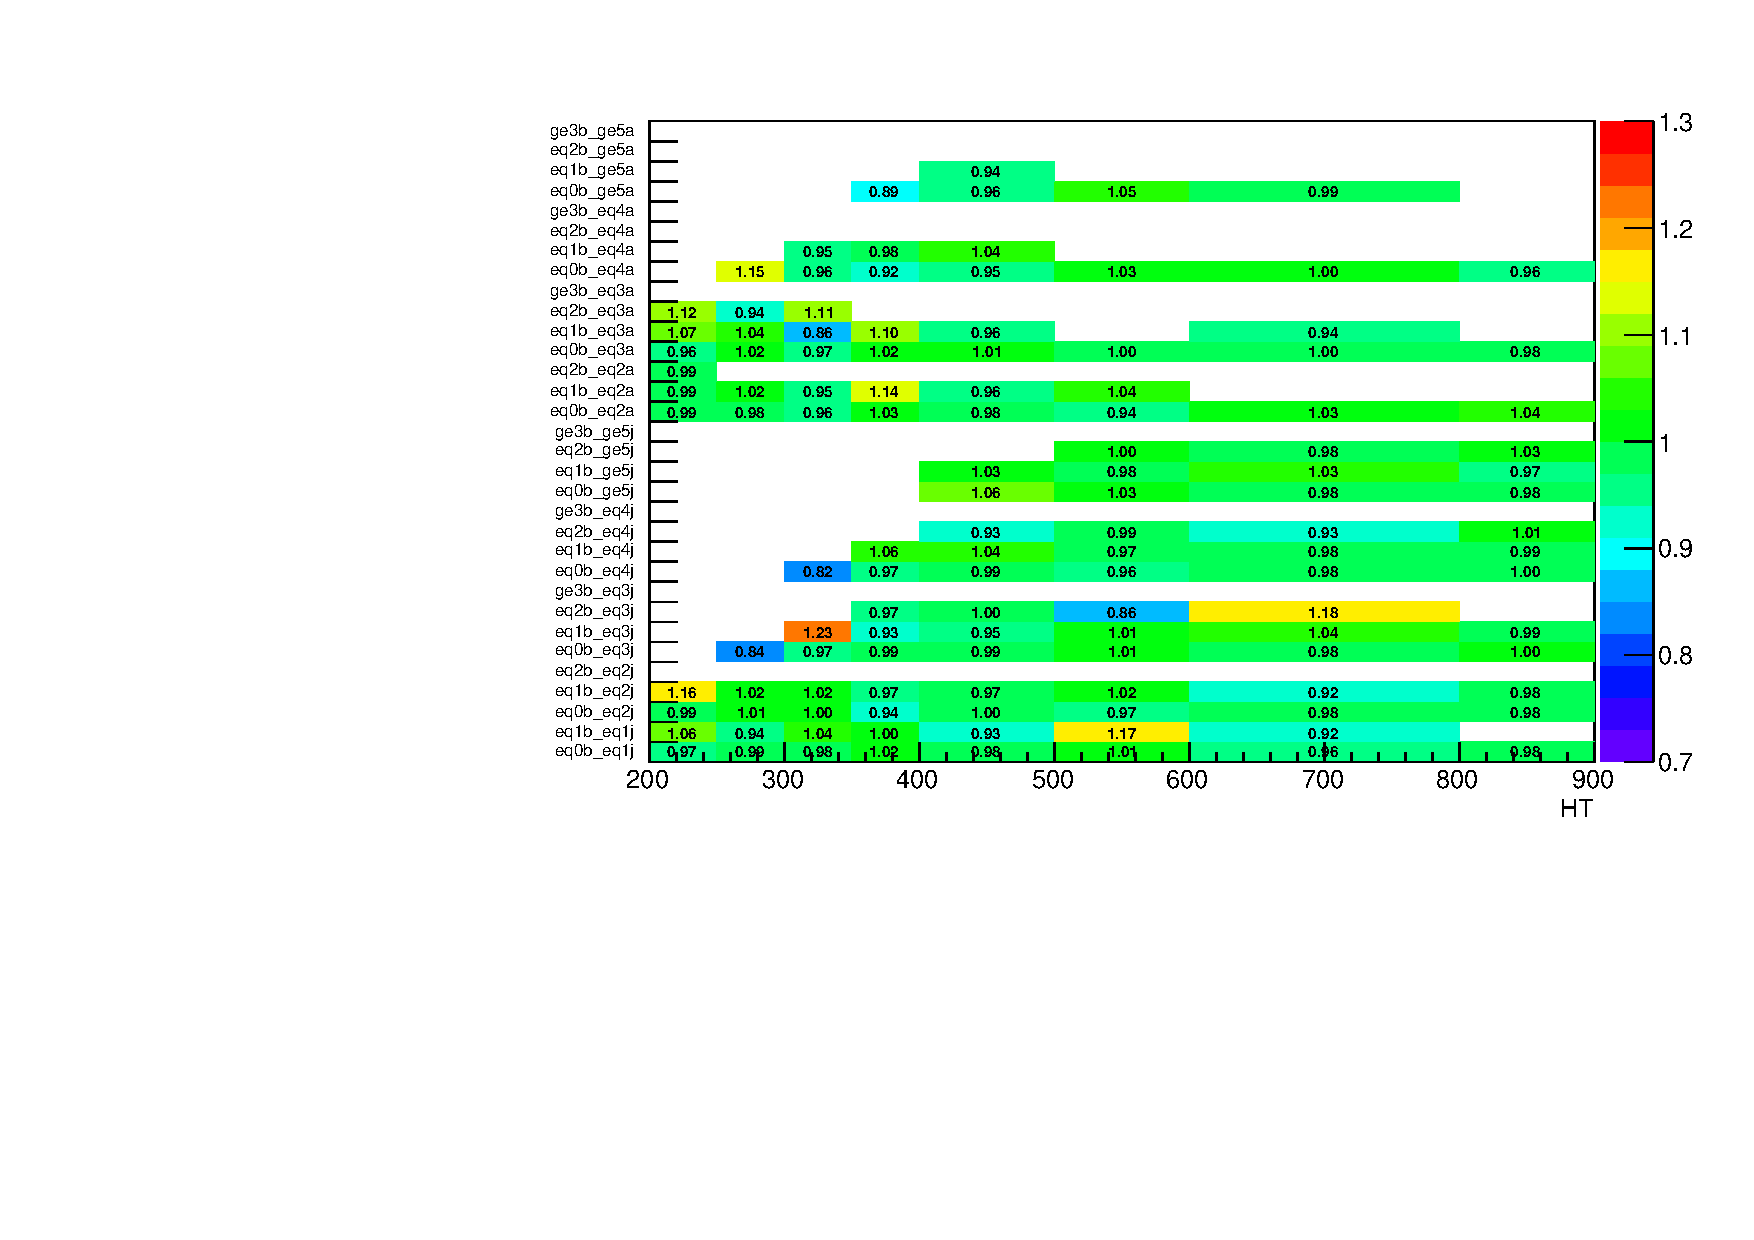
\includegraphics[width=0.5\textwidth]{figures/mcSystematics/Zinv/mumu/ratiotfh_ht_mht_alljecWeight_Down.pdf}
  }\\
  \subfigure[B-tag scale factors varied up]{
    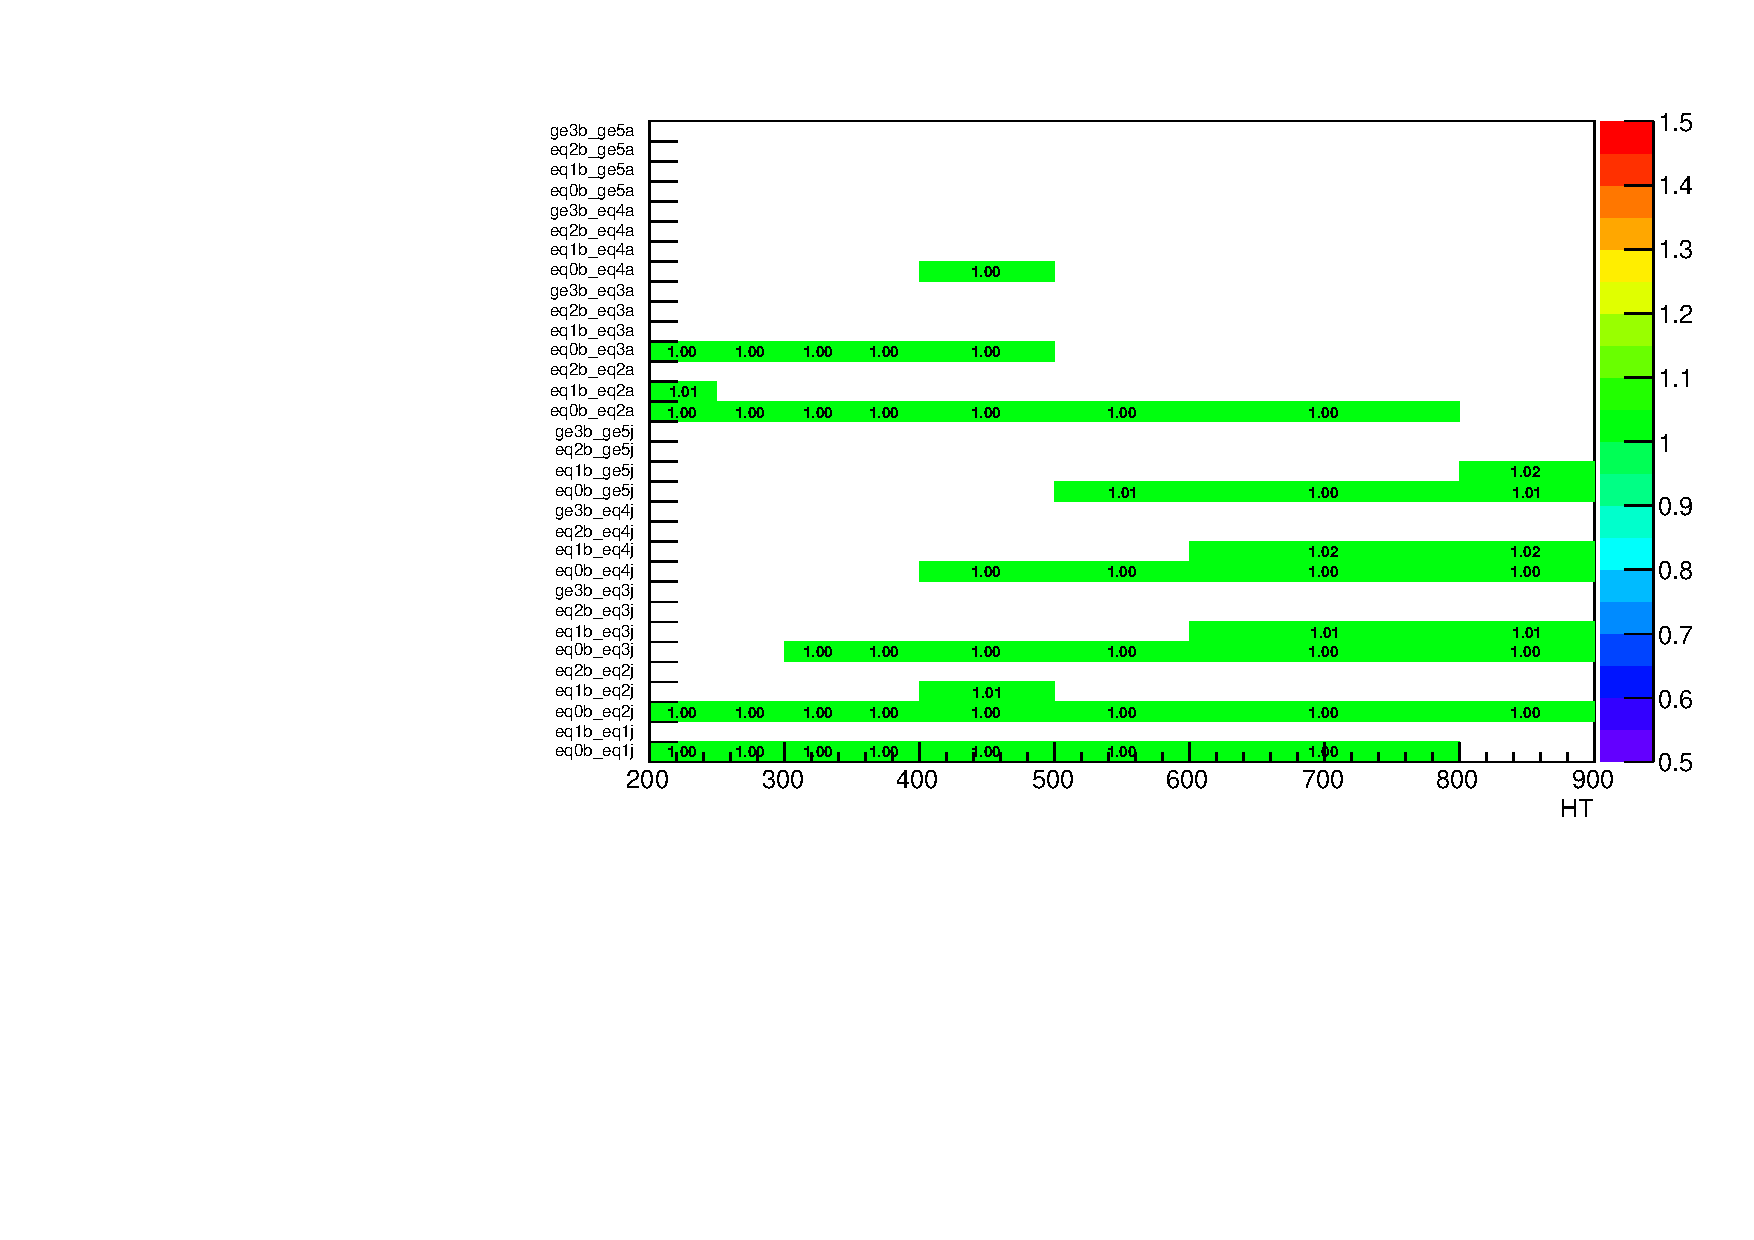
\includegraphics[width=0.5\textwidth]{figures/mcSystematics/Zinv/mumu/ratiotfh_ht_mht_allbsfWeight_Up.pdf}
  } ~~
  \subfigure[B-tag scale factors varied down]{
    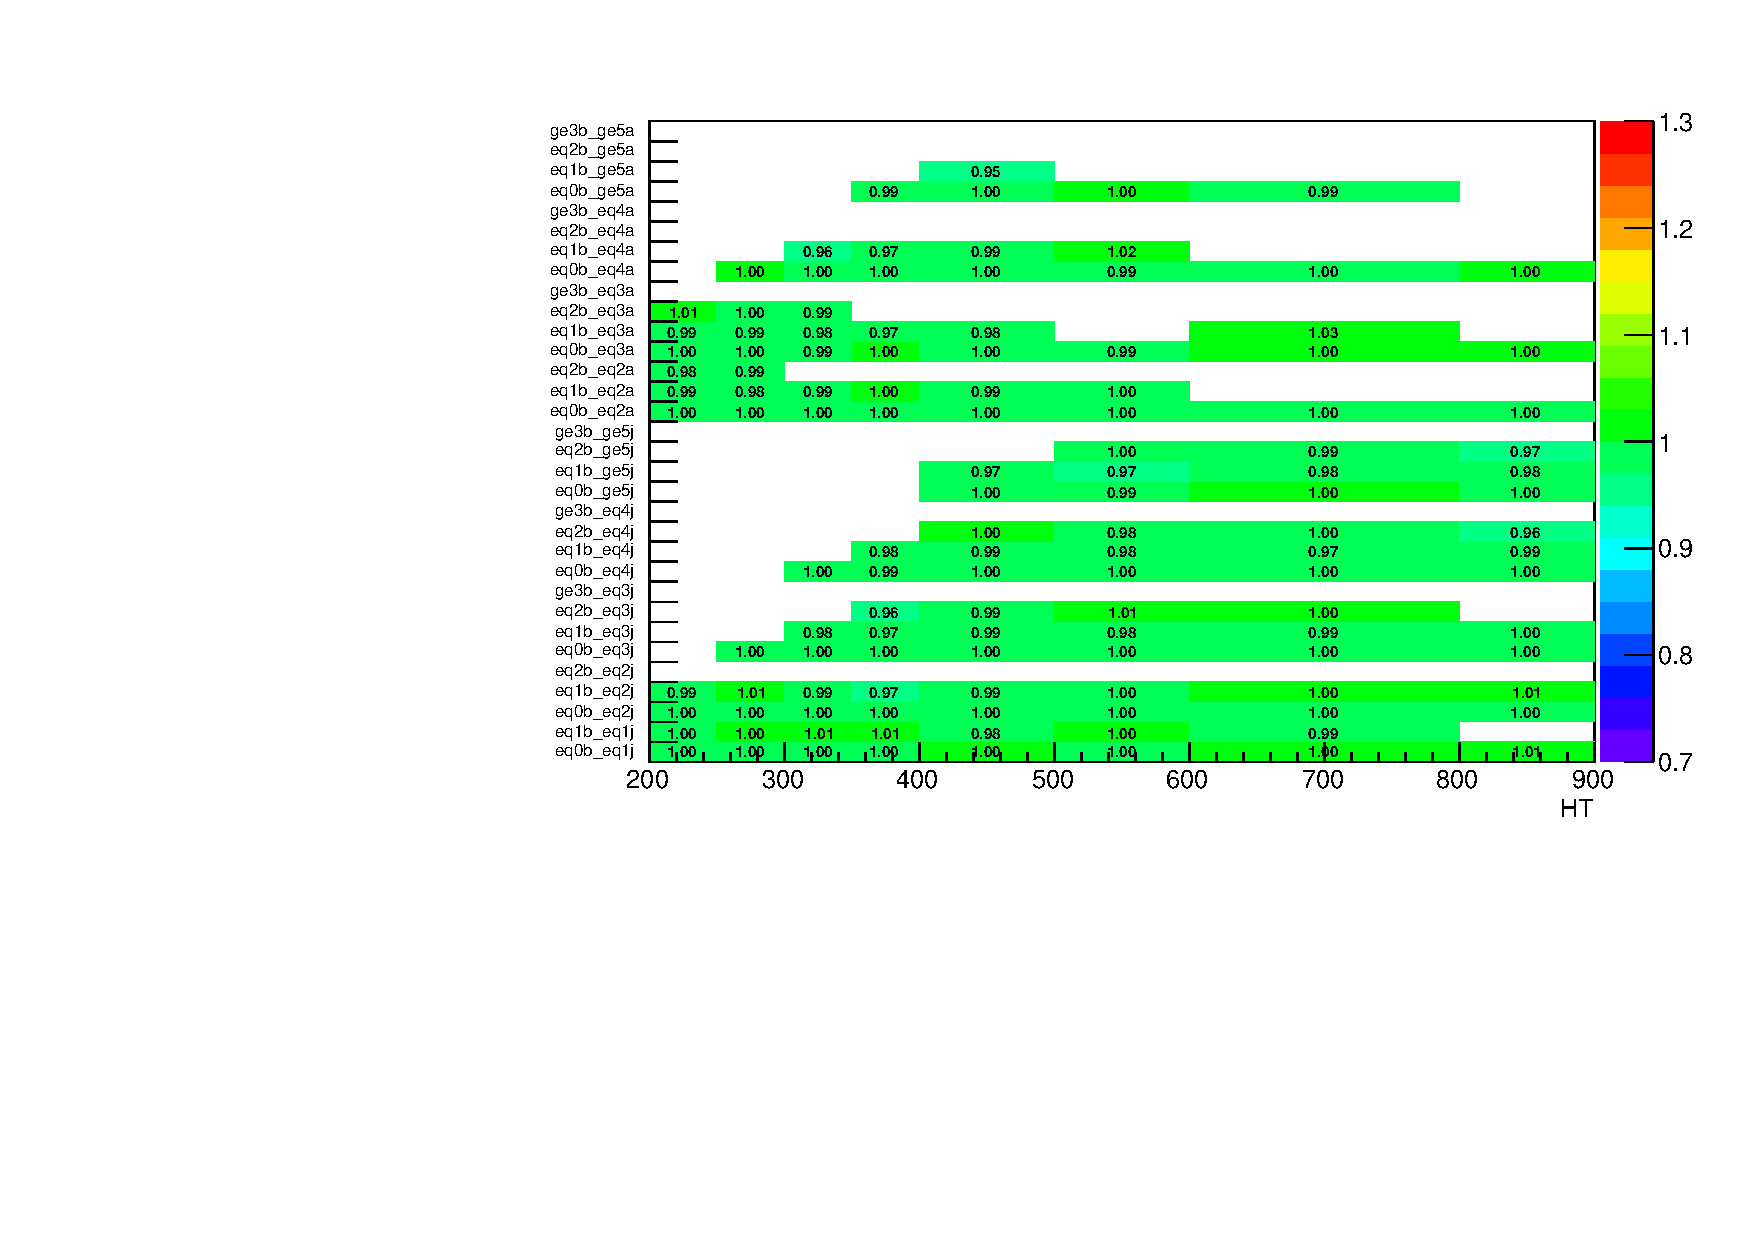
\includegraphics[width=0.5\textwidth]{figures/mcSystematics/Zinv/mumu/ratiotfh_ht_mht_allbsfWeight_Down.pdf}
  }\\
  \subfigure[Pileup weights factors varied up]{
    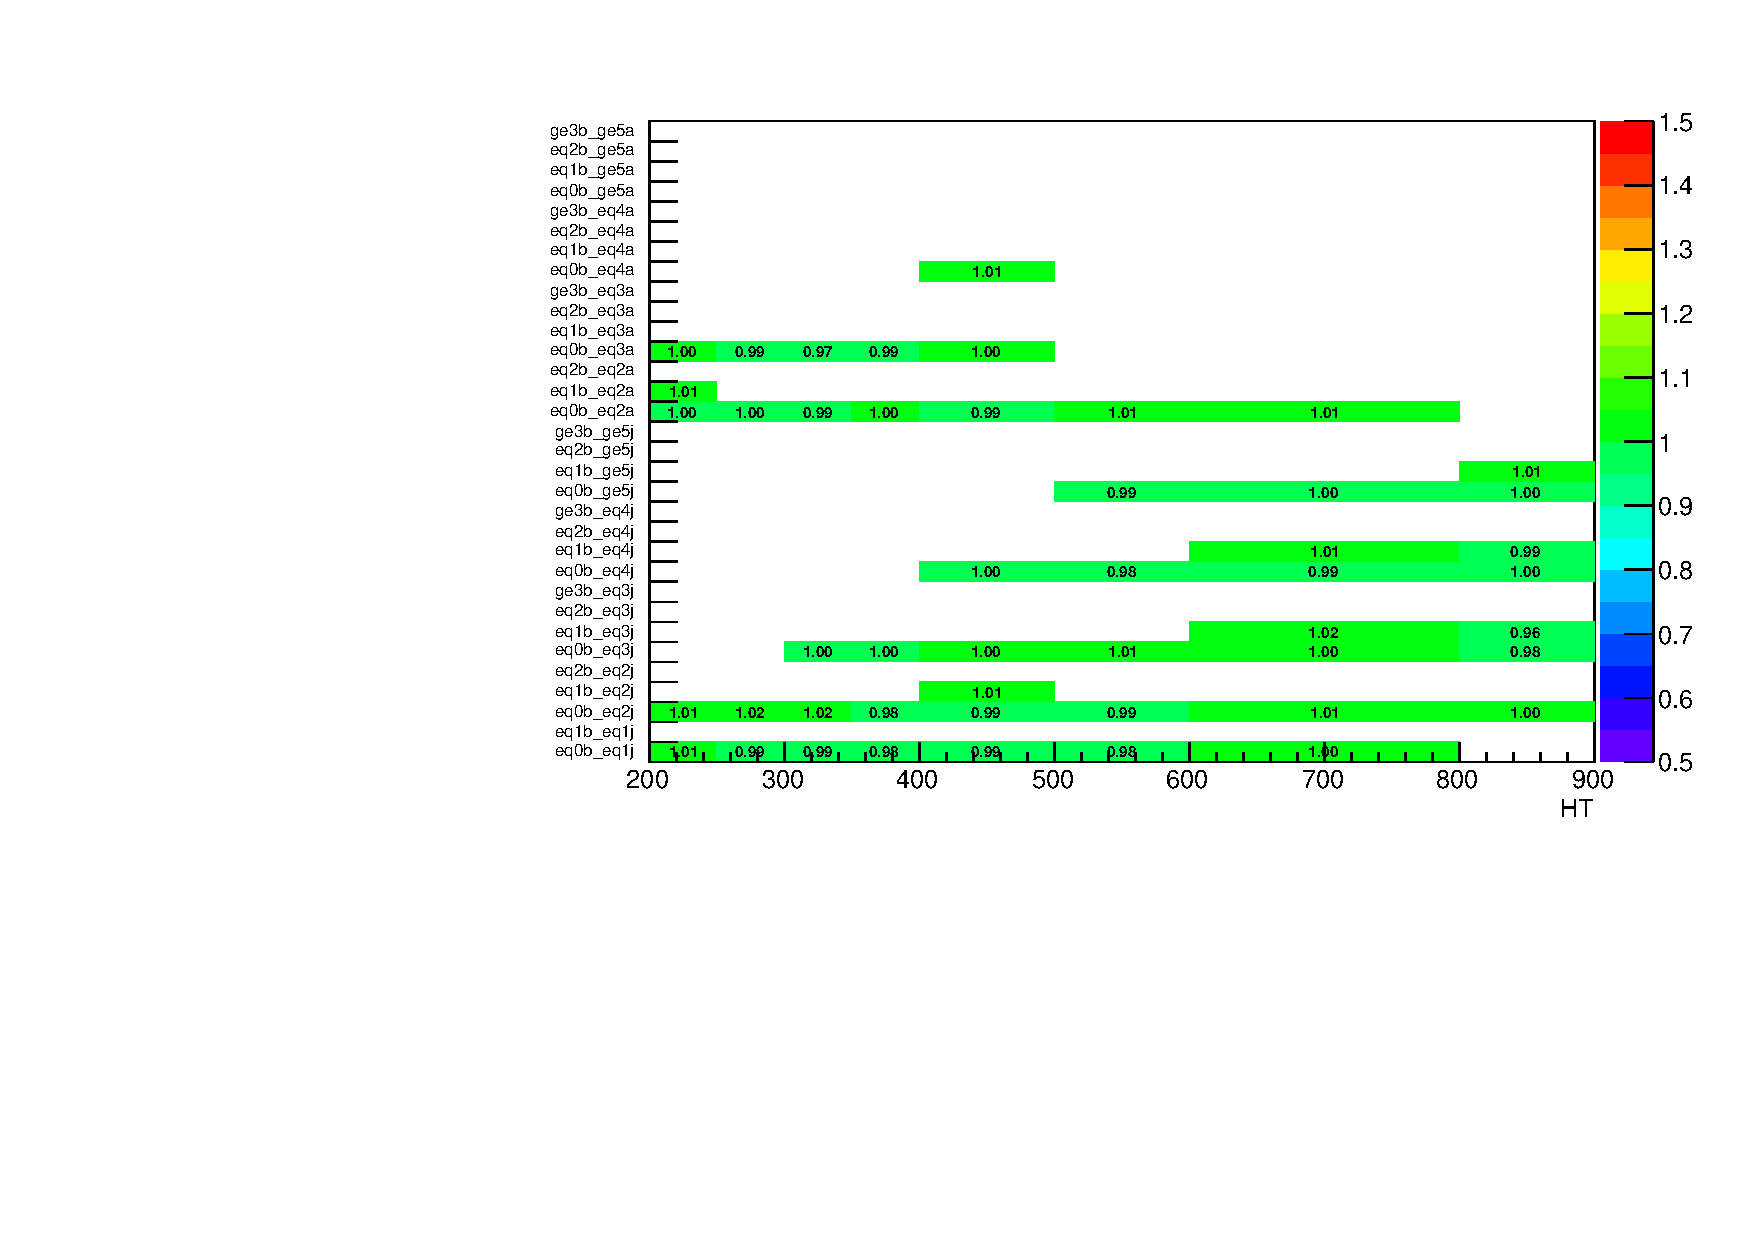
\includegraphics[width=0.5\textwidth]{figures/mcSystematics/Zinv/mumu/ratiotfh_ht_mht_allpuWeight_Up.pdf}
  } ~~
  \subfigure[Pileup weights factors varied down]{
    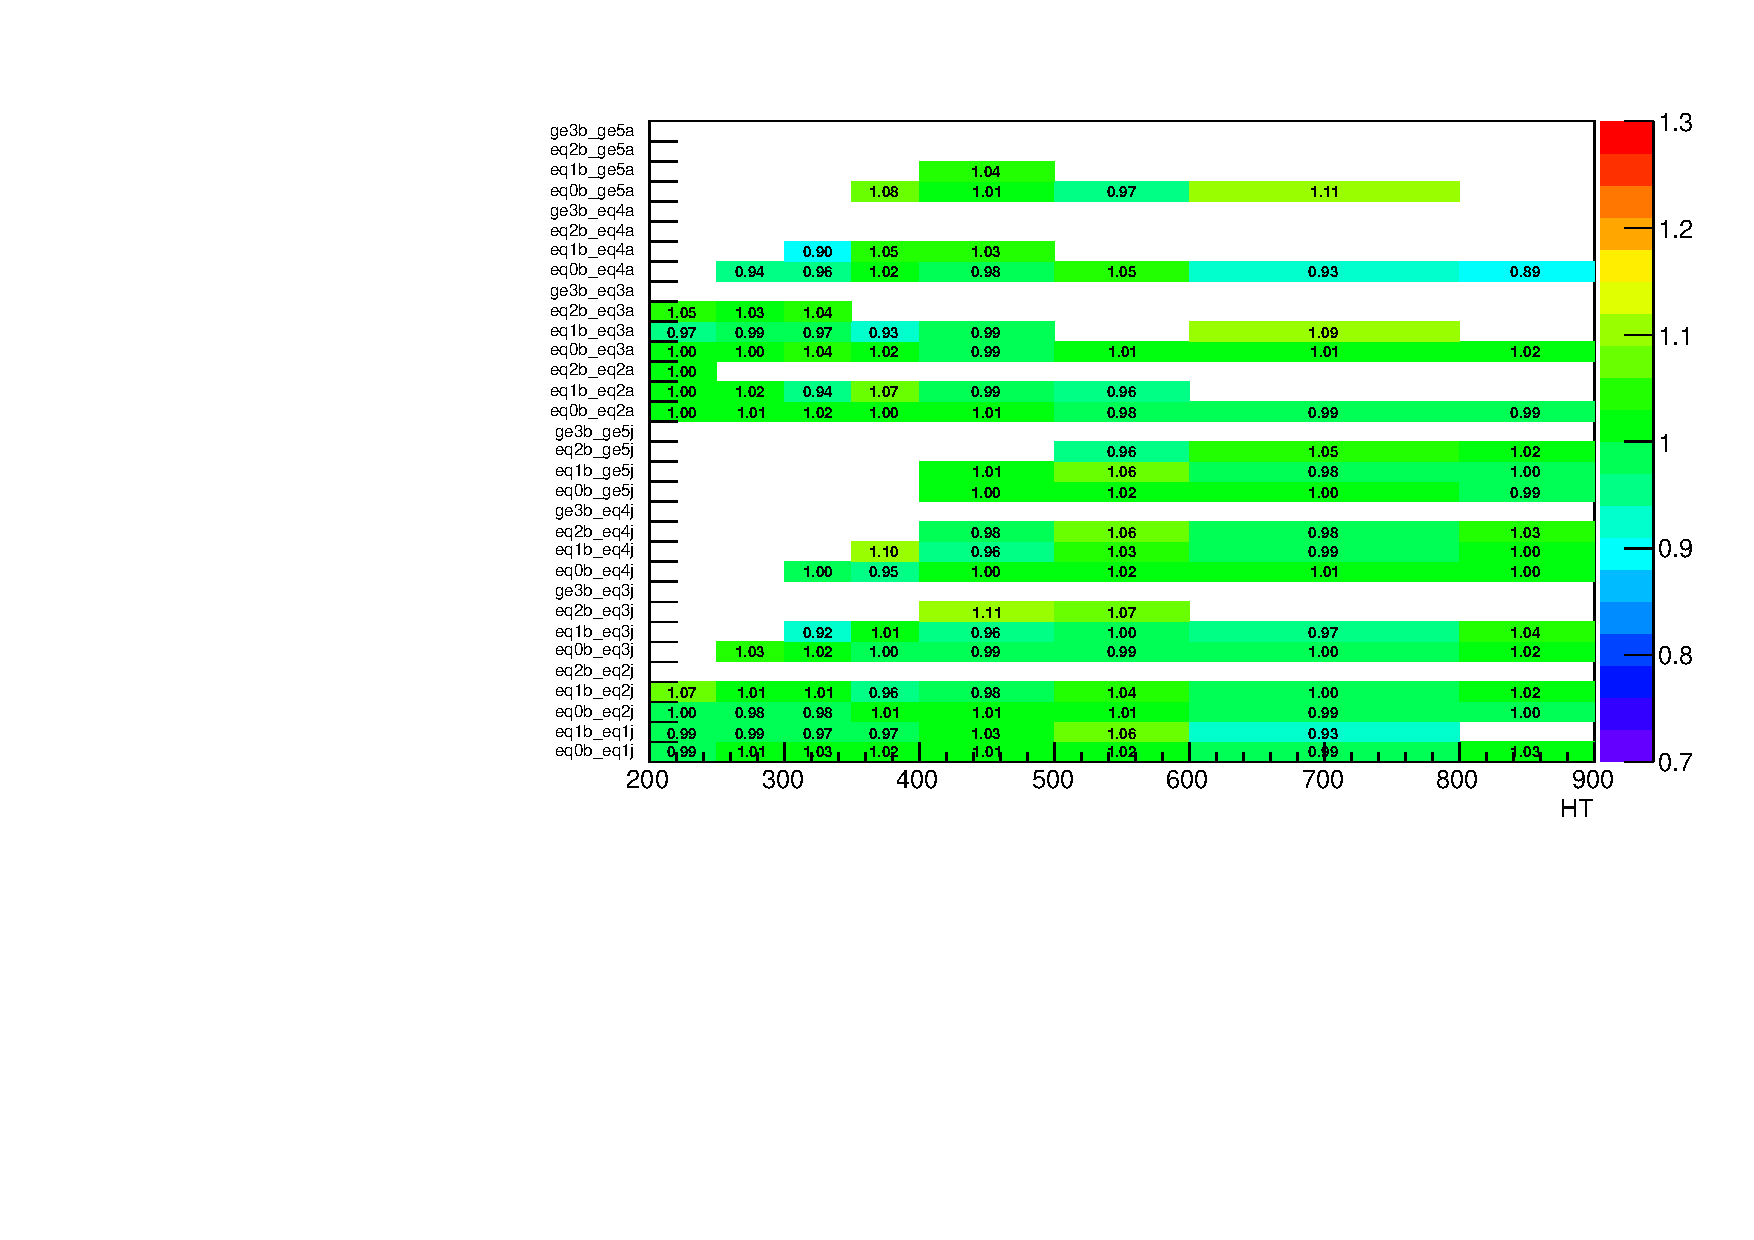
\includegraphics[width=0.5\textwidth]{figures/mcSystematics/Zinv/mumu/ratiotfh_ht_mht_allpuWeight_Down.pdf}
  }\\
  \subfigure[Top $p_{T}$ weights varied up]{
    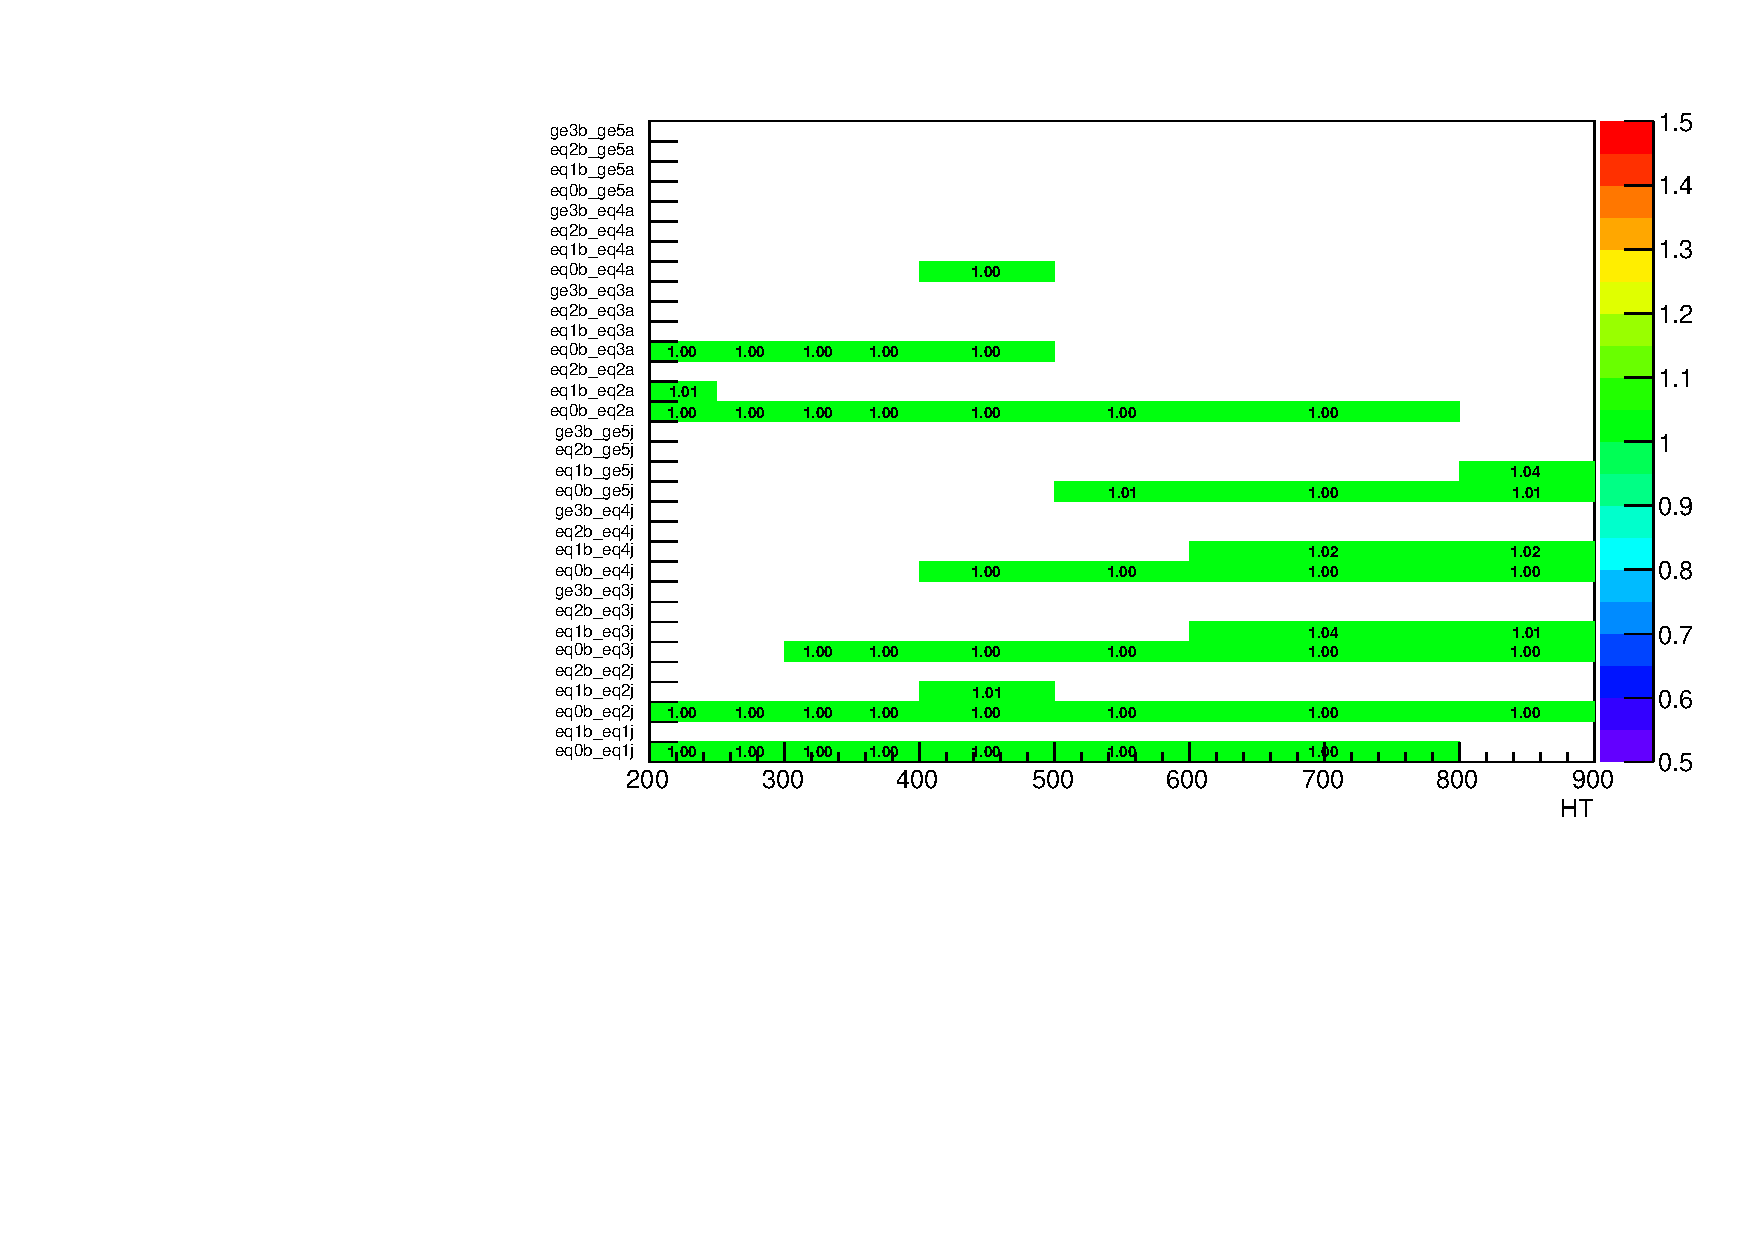
\includegraphics[width=0.5\textwidth]{figures/mcSystematics/Zinv/mumu/ratiotfh_ht_mht_alltopPtWeight_Up.pdf}
  } ~~
  \subfigure[Top $p_{T}$ weights varied down]{
    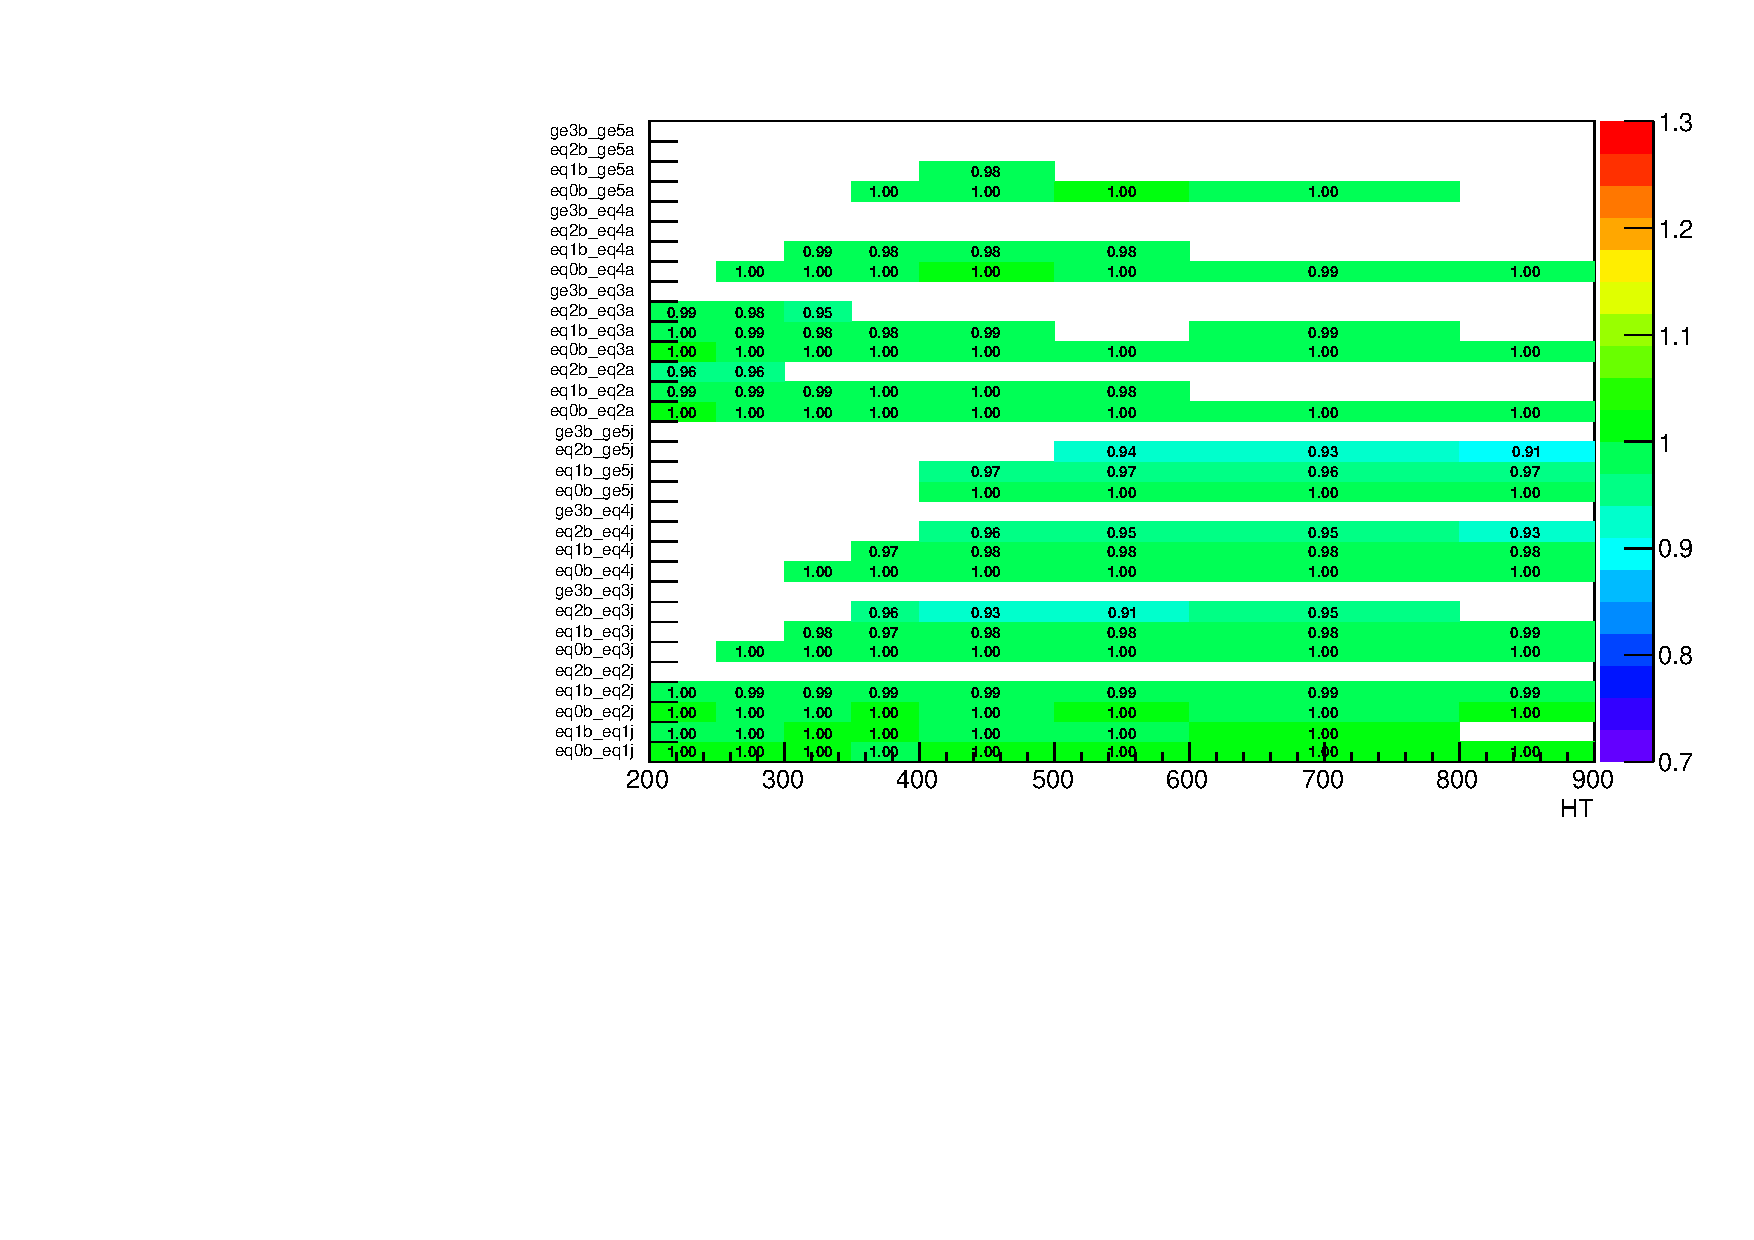
\includegraphics[width=0.5\textwidth]{figures/mcSystematics/Zinv/mumu/ratiotfh_ht_mht_alltopPtWeight_Down.pdf}
  }\\
  \caption{\label{fig:mumuZnunuTF} The change in \mmj to \znunu transfer
  factors when varying various parameters in the MC simulation by
  there upwards and downwards one sigma values. }
\end{figure}

{\bf Data-driven systematics}

The result of the \alphat and $\Delta\phi *$ closure tests contribute
to the systematic uncertainty as described in Sec.~\ref{sec:muZnunu}.

\subsubsection{Tests probing the prediction of the \znunu
background with the \gj control sample}

{\bf Variations on the transfer factors from simulation}

All the MC variations described in Sec~\ref{sec:mc-systematics} are
carried out for the transfer factors from the \gj control region to
the \znunu background prediction. The results are shown in
Fig.~\ref{gZnunuTF}.

\begin{figure}[]
  \centering
  \subfigure[Jet energy scale varied up]{
    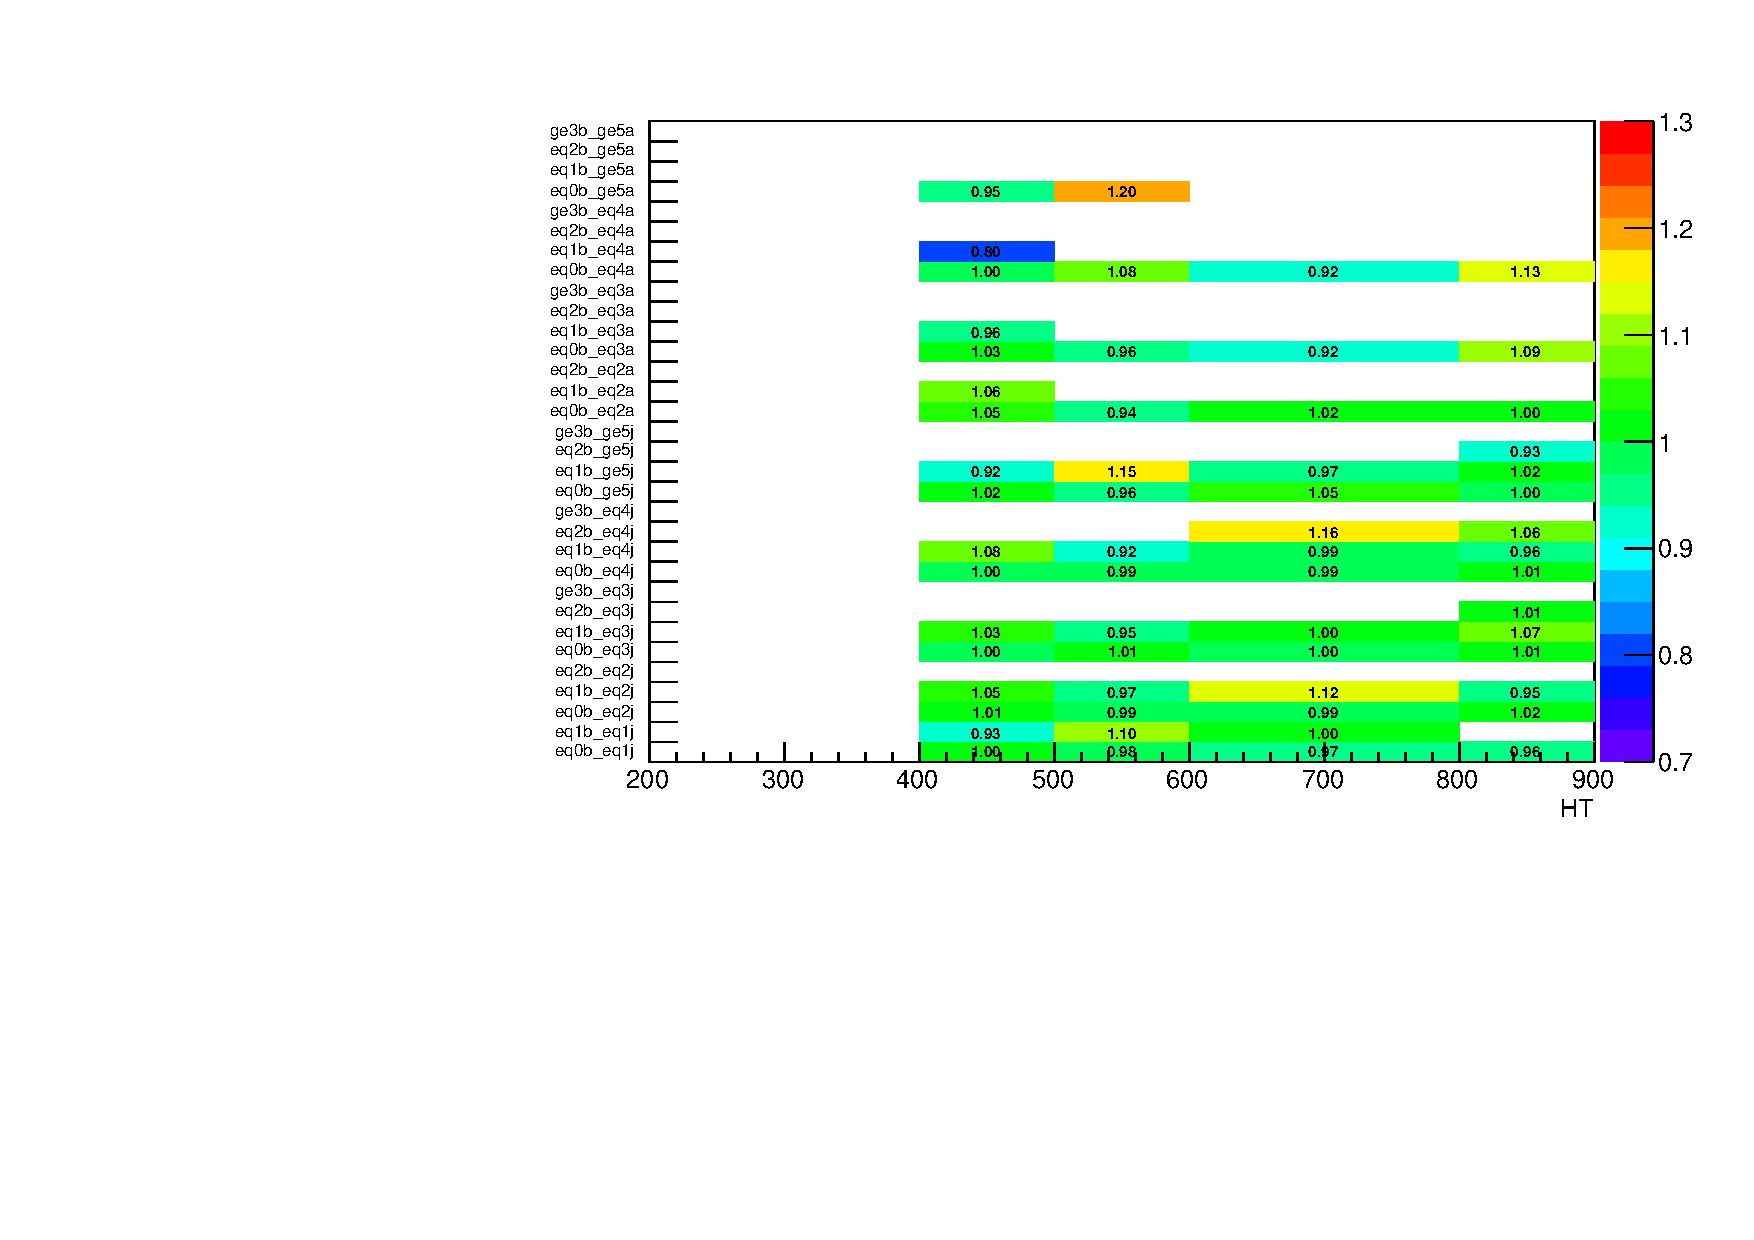
\includegraphics[width=0.5\textwidth]{figures/mcSystematics/Zinv/gj/ratiotfh_ht_mht_alljecWeight_Up.pdf}
  } ~~
  \subfigure[Jet energy scale varied down]{
    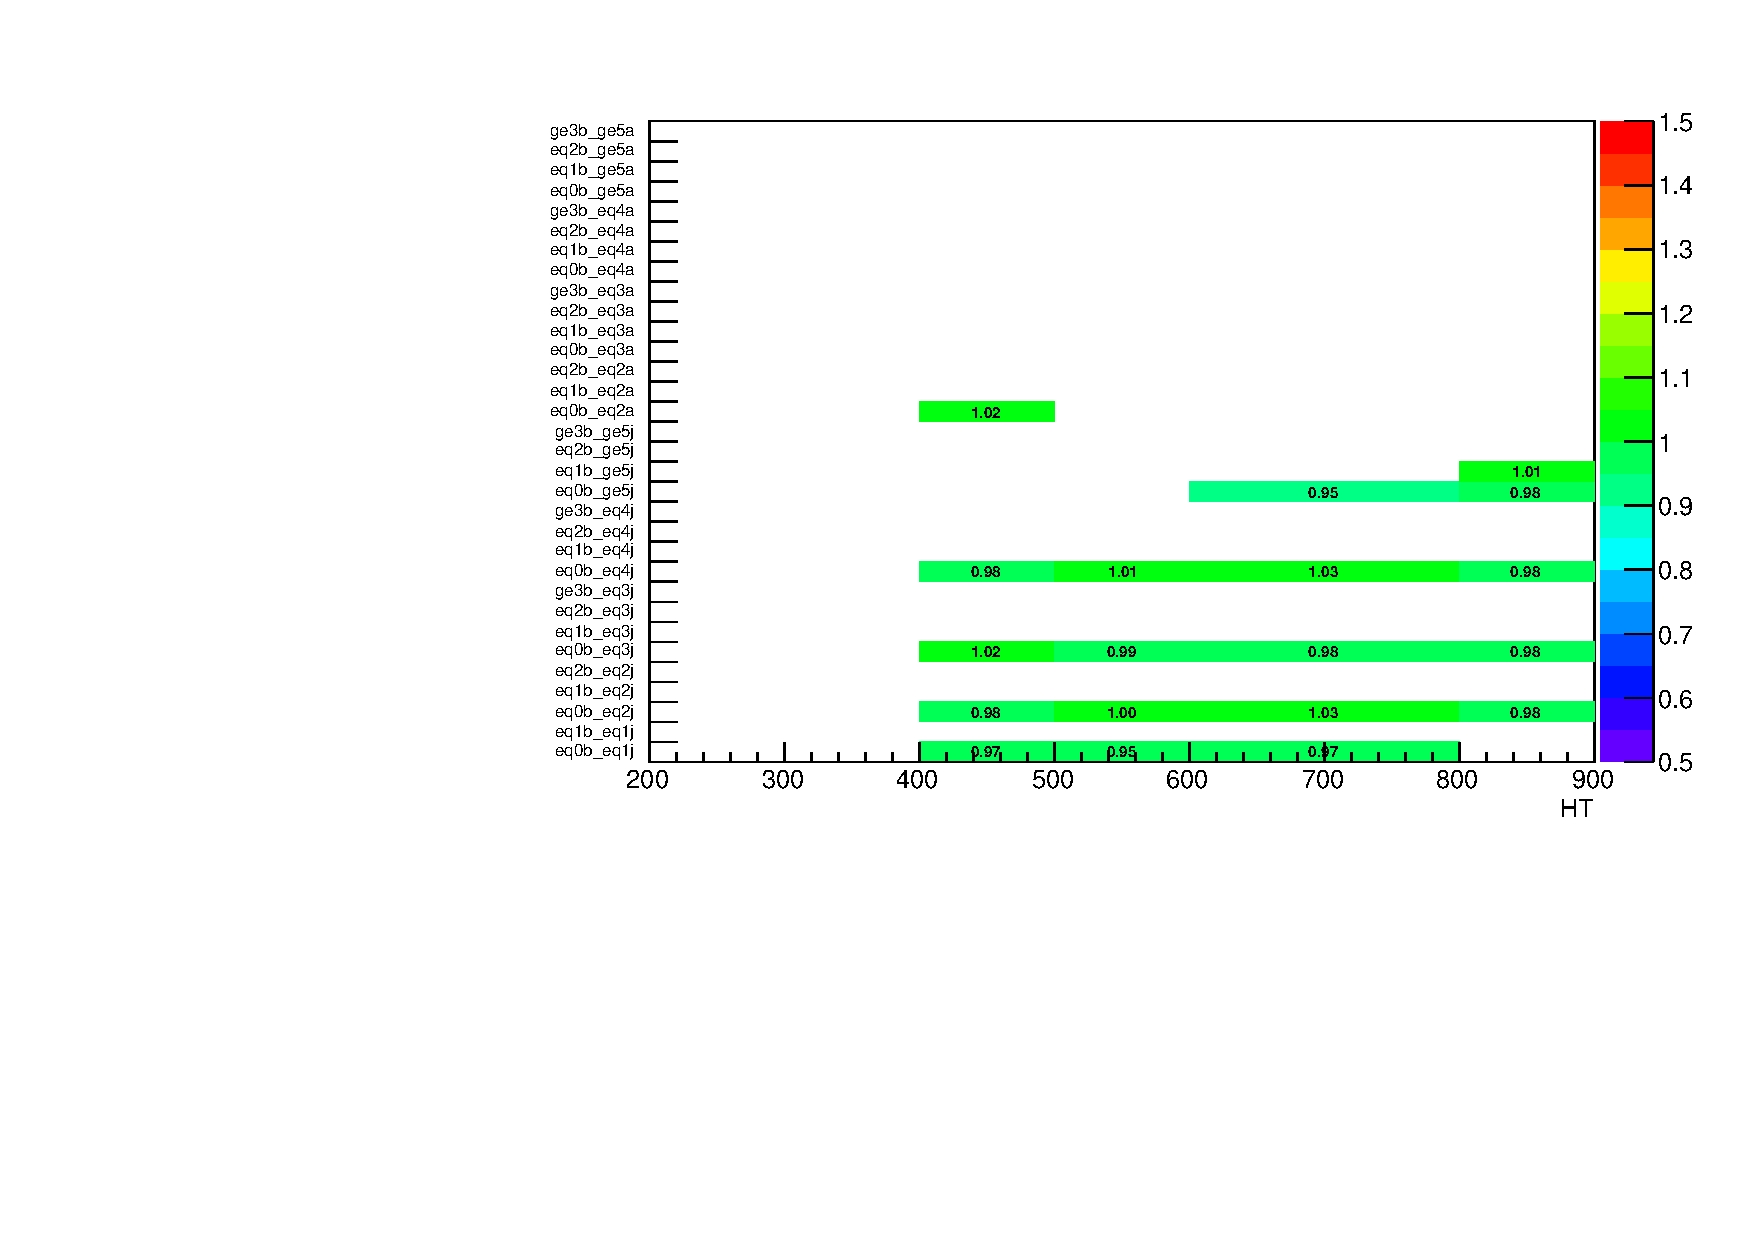
\includegraphics[width=0.5\textwidth]{figures/mcSystematics/Zinv/gj/ratiotfh_ht_mht_alljecWeight_Down.pdf}
  }\\
  \subfigure[B-tag scale factors varied up]{
    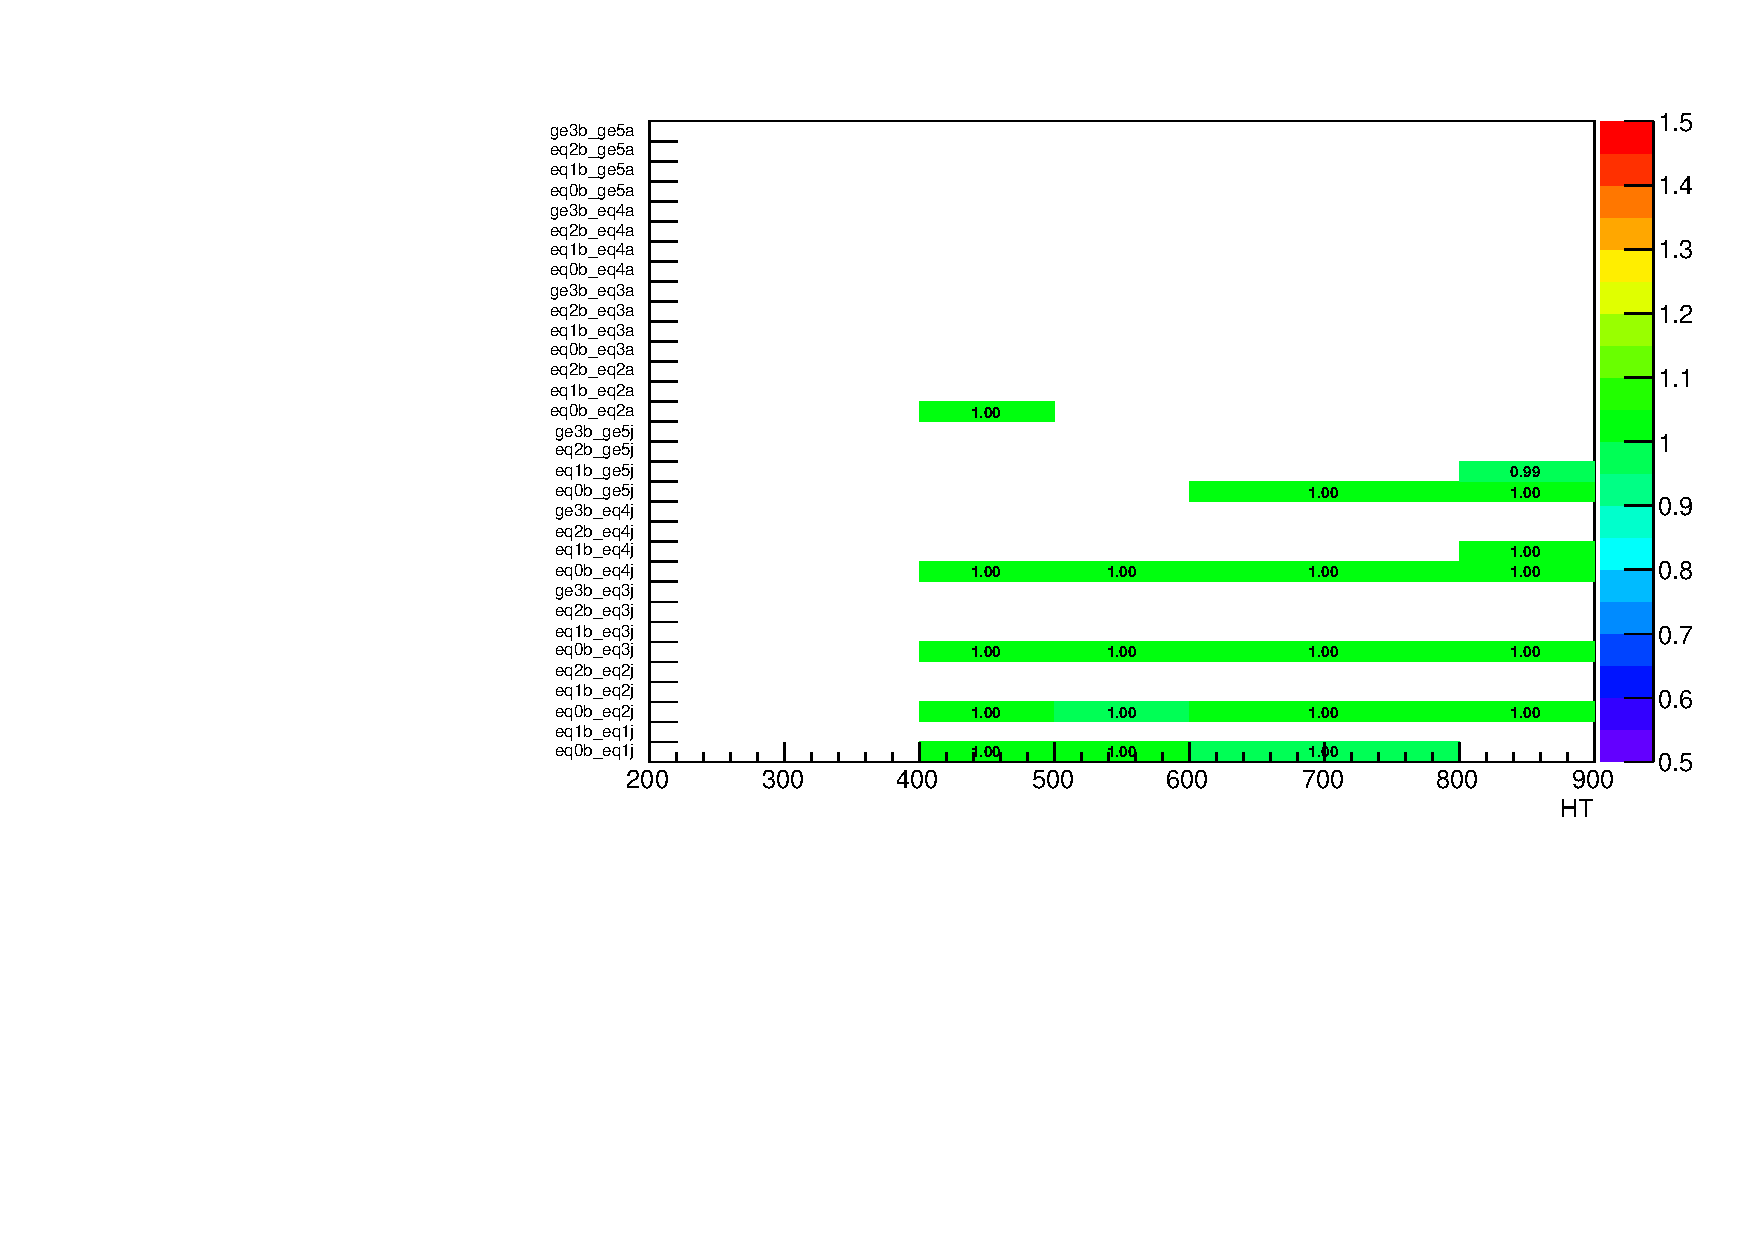
\includegraphics[width=0.5\textwidth]{figures/mcSystematics/Zinv/gj/ratiotfh_ht_mht_allbsfWeight_Up.pdf}
  } ~~
  \subfigure[B-tag scale factors varied down]{
    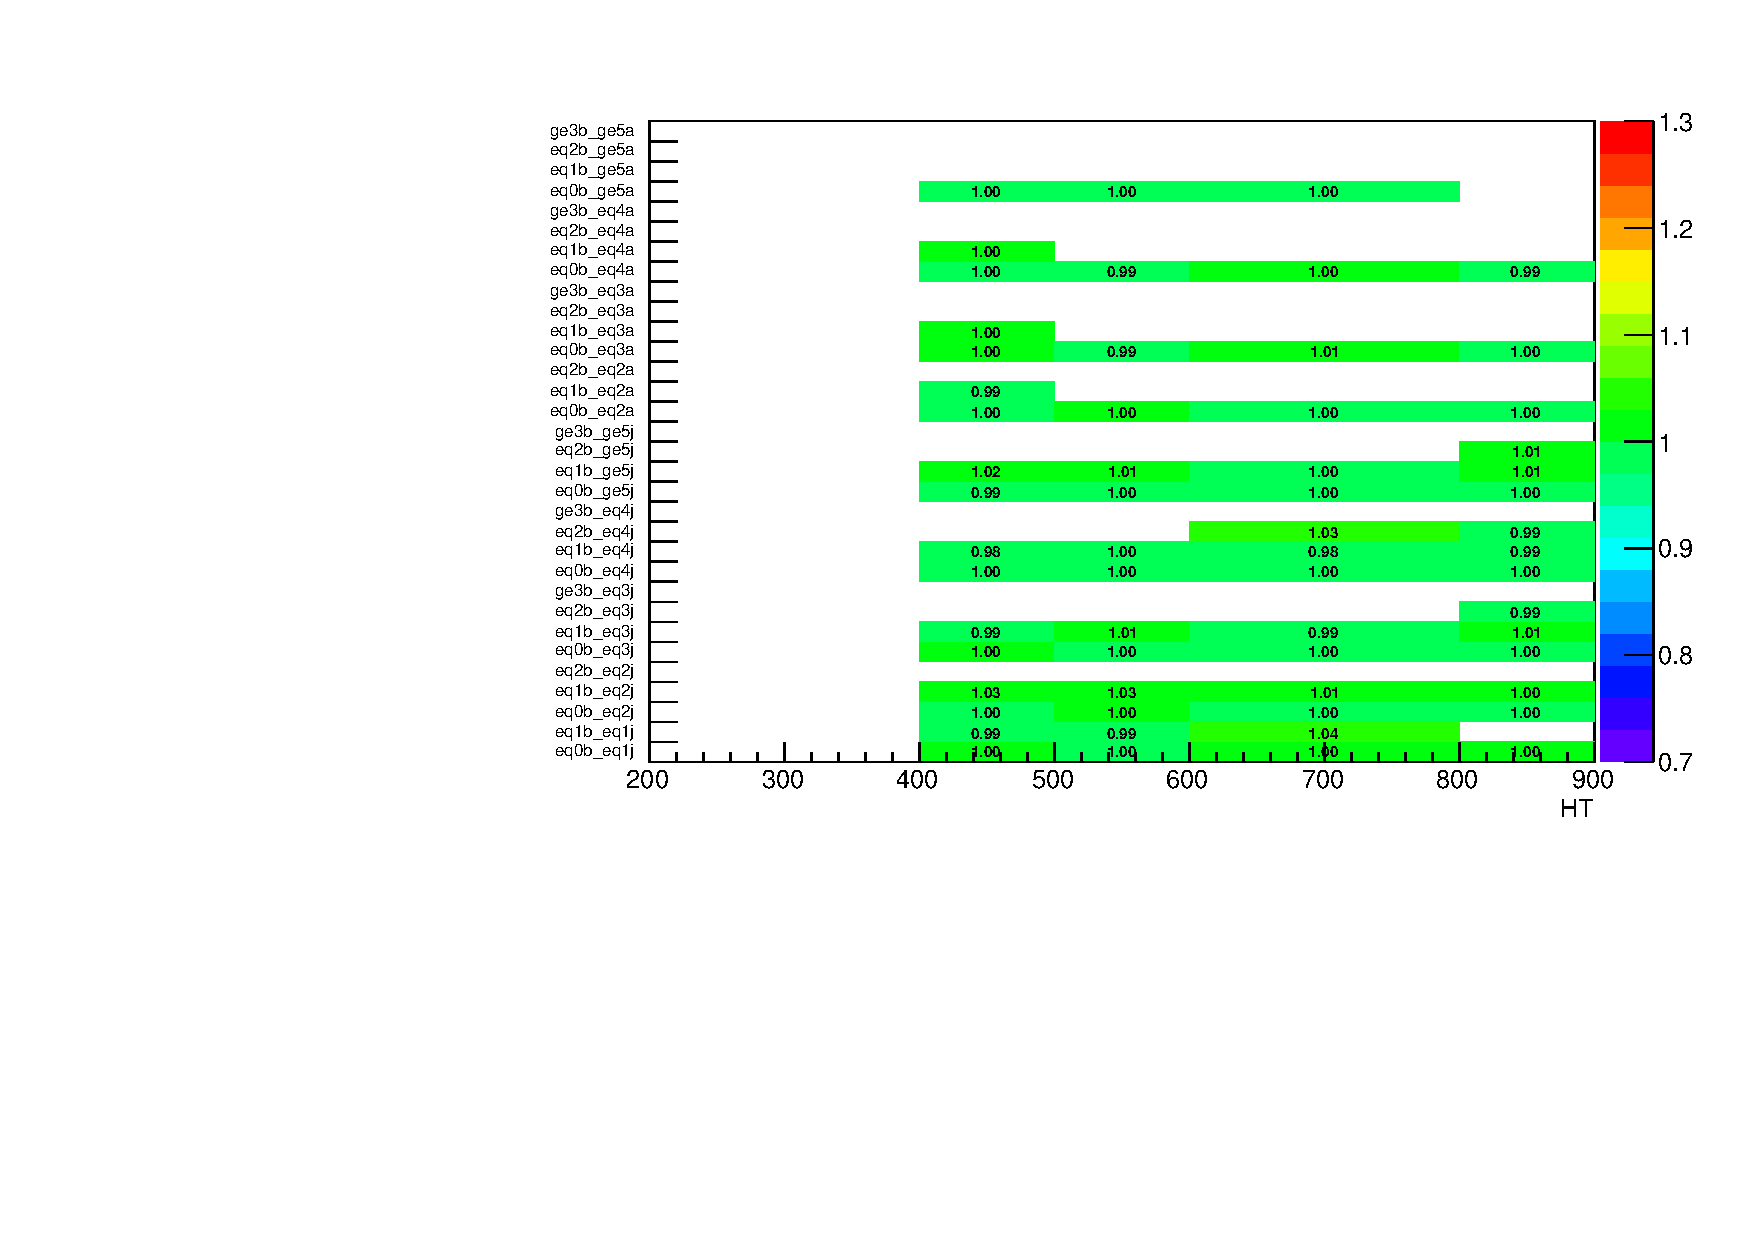
\includegraphics[width=0.5\textwidth]{figures/mcSystematics/Zinv/gj/ratiotfh_ht_mht_allbsfWeight_Down.pdf}
  }\\
  \subfigure[Pileup weights factors varied up]{
    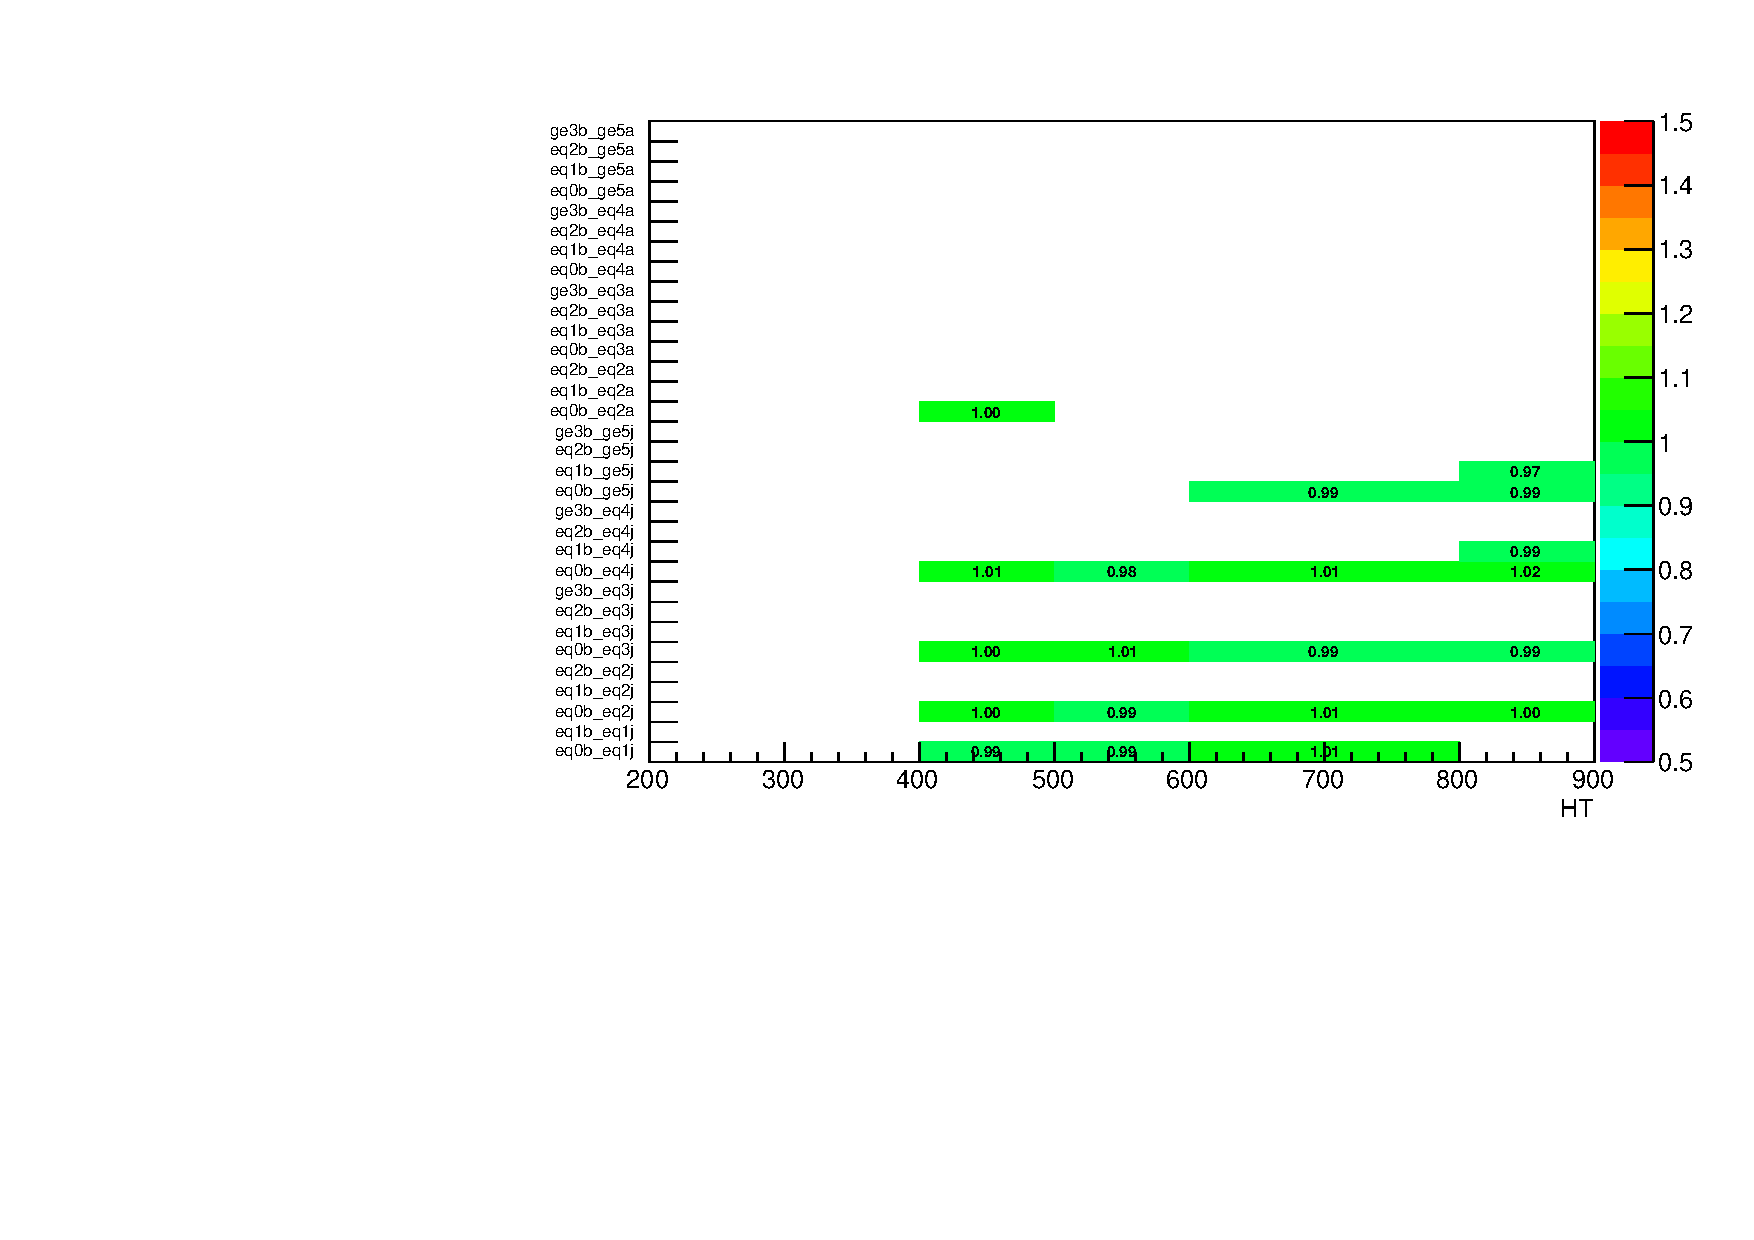
\includegraphics[width=0.5\textwidth]{figures/mcSystematics/Zinv/gj/ratiotfh_ht_mht_allpuWeight_Up.pdf}
  } ~~
  \subfigure[Pileup weights factors varied down]{
    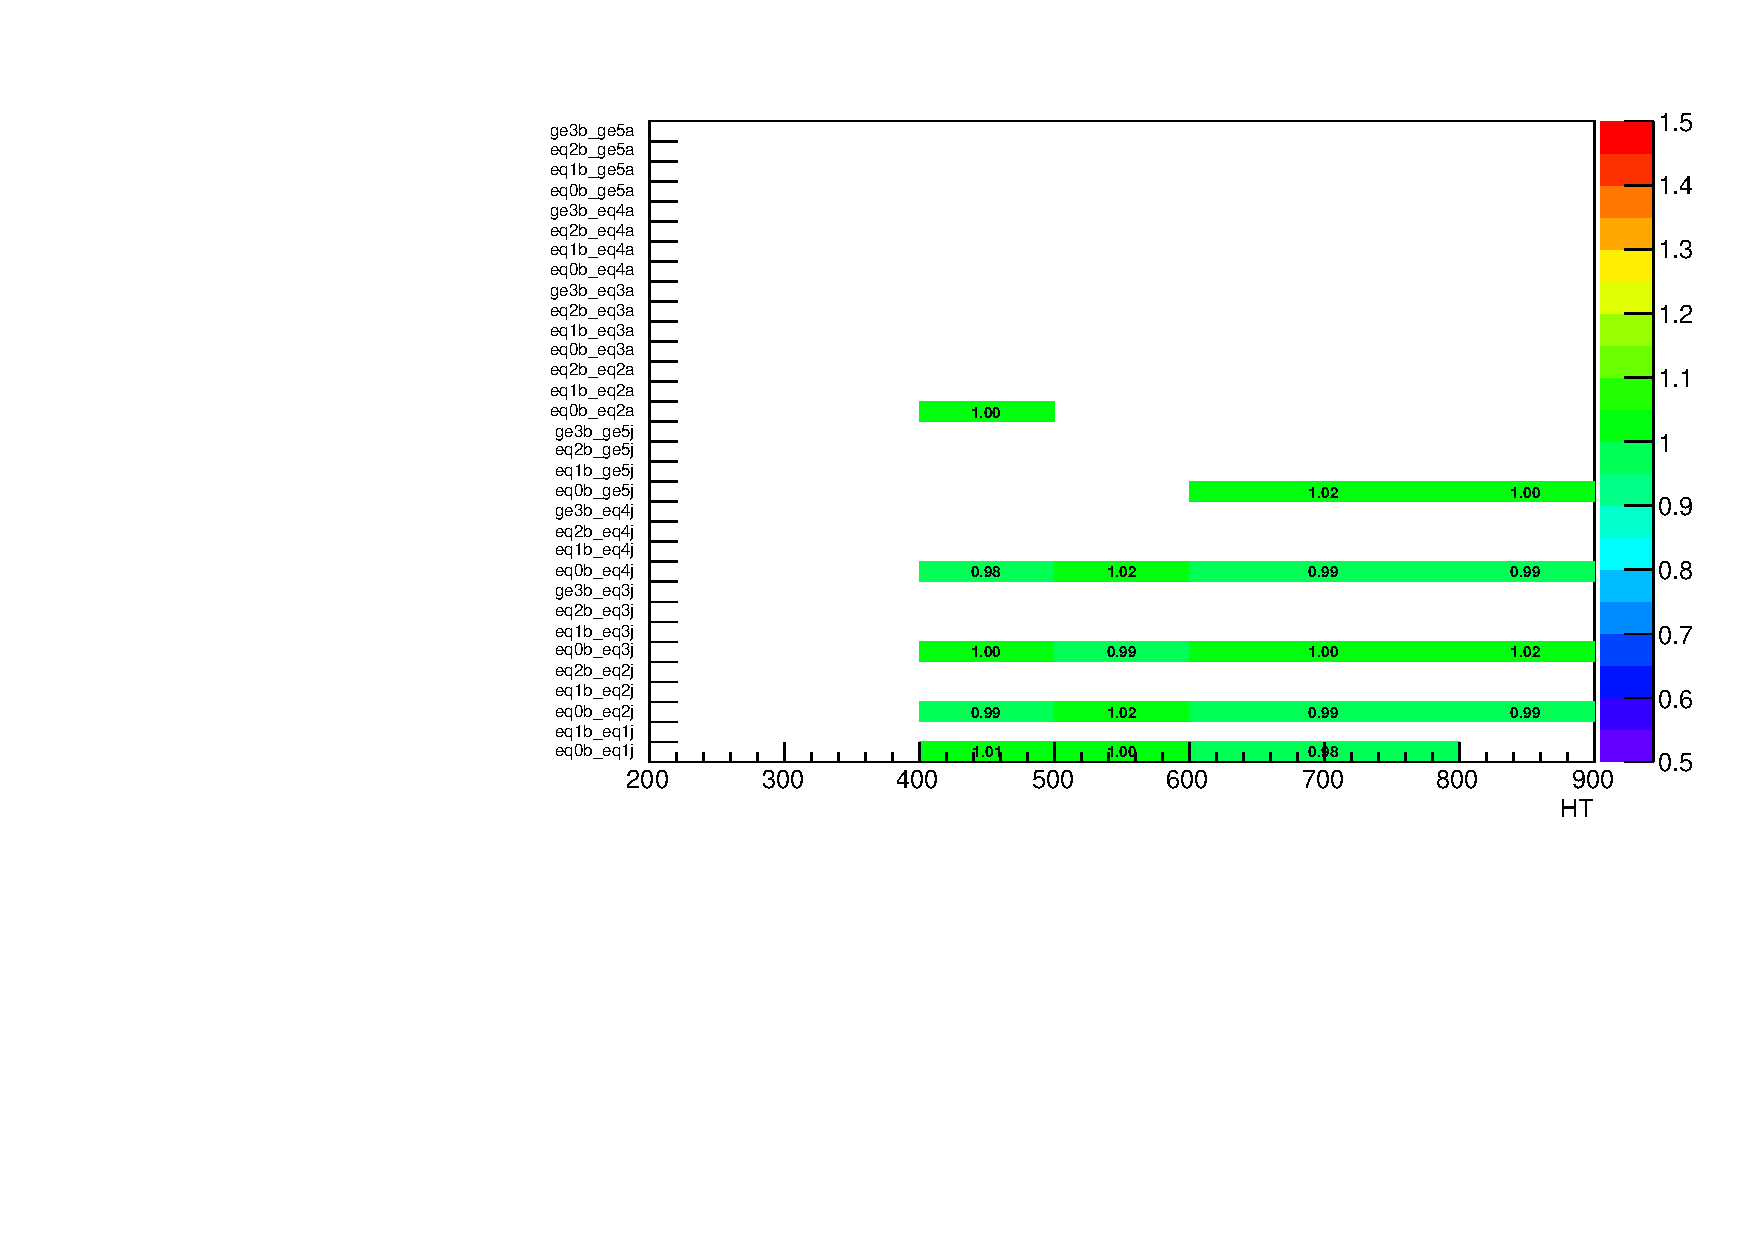
\includegraphics[width=0.5\textwidth]{figures/mcSystematics/Zinv/gj/ratiotfh_ht_mht_allpuWeight_Down.pdf}
  }\\
  \subfigure[Top $p_{T}$ weights varied up]{
    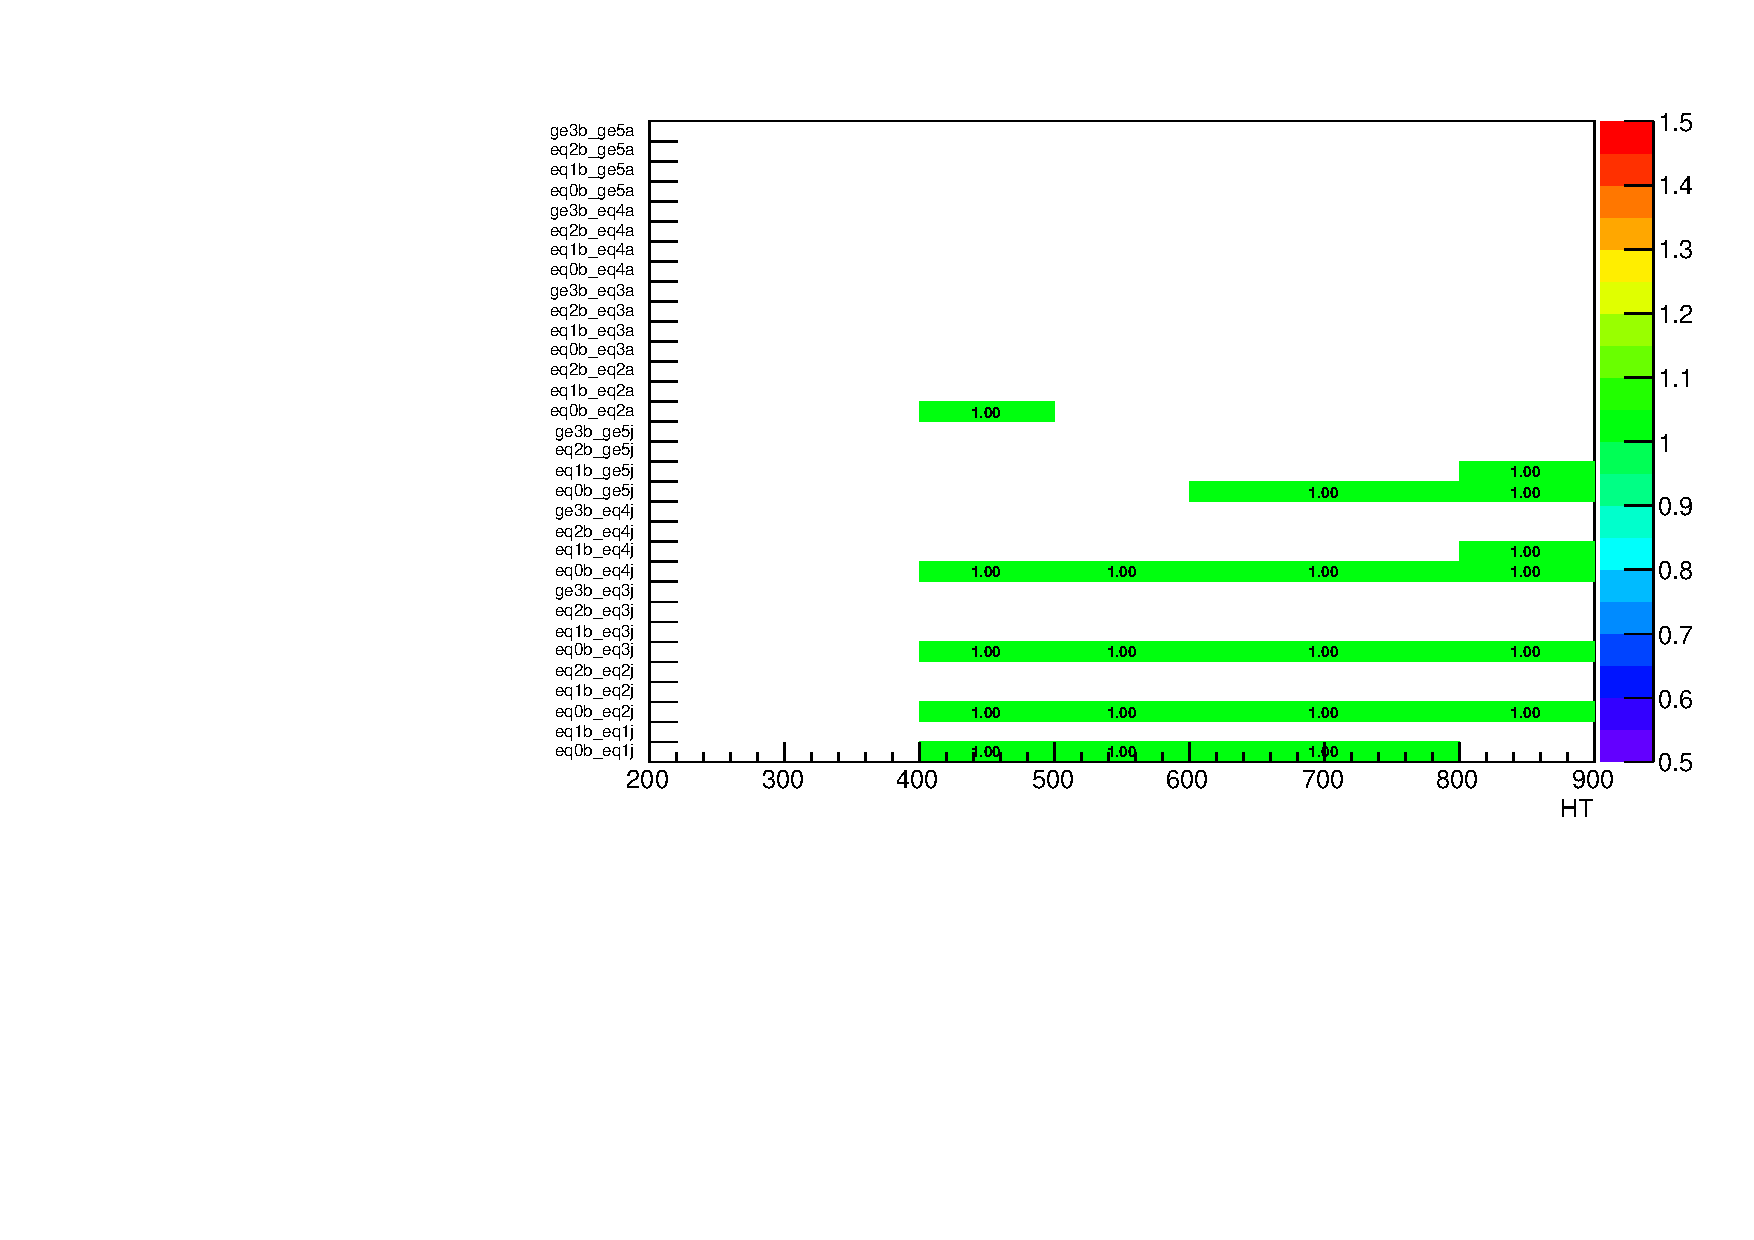
\includegraphics[width=0.5\textwidth]{figures/mcSystematics/Zinv/gj/ratiotfh_ht_mht_alltopPtWeight_Up.pdf}
  } ~~
  \subfigure[Top $p_{T}$ weights varied down]{
    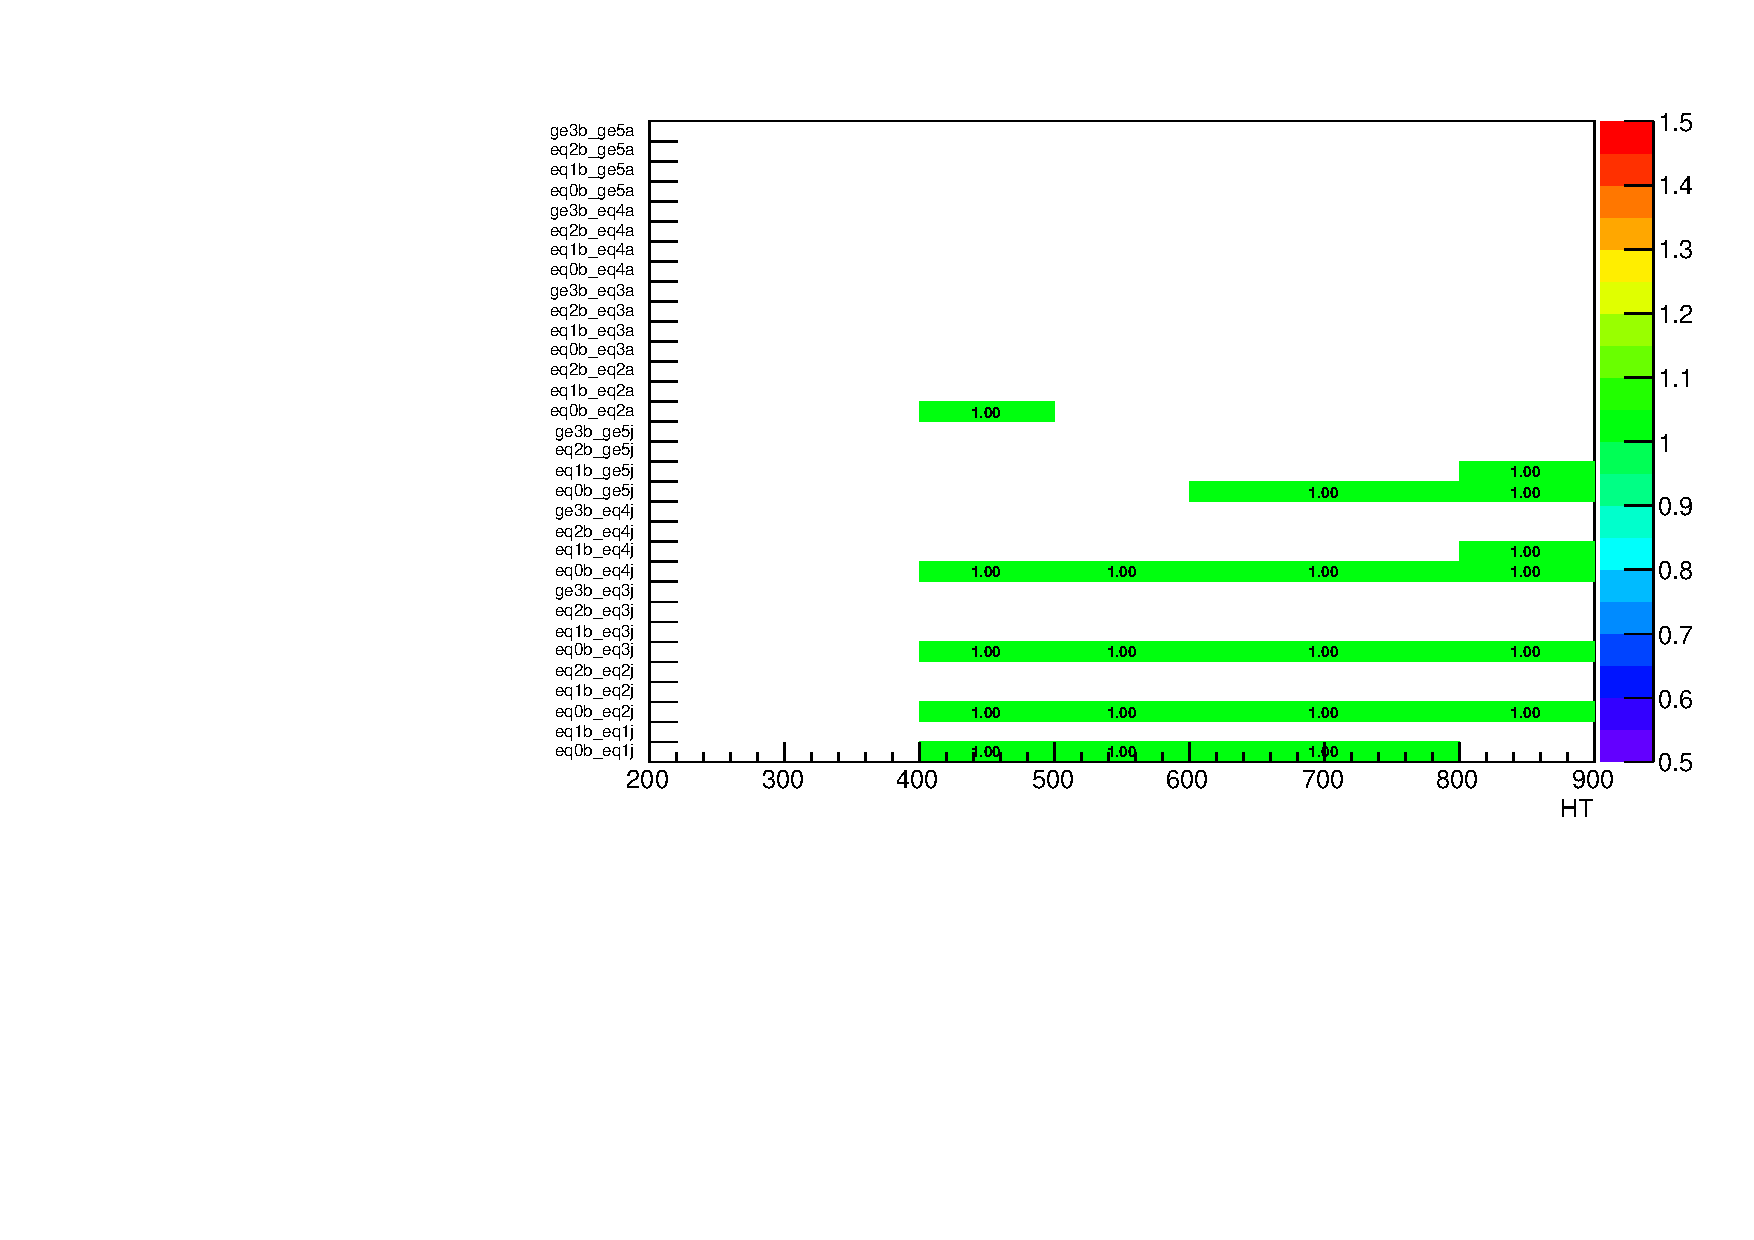
\includegraphics[width=0.5\textwidth]{figures/mcSystematics/Zinv/gj/ratiotfh_ht_mht_alltopPtWeight_Down.pdf}
  }\\
  \caption{\label{fig:gZnunuTF} The change in \gj to \znunu transfer
  factors when varying various parameters in the MC simulation by
  there upwards and downwards one sigma values. }
\end{figure}

{\bf Data-driven systematics}

To test the use of a \gj sample to predict the \zinv background, $\gj
\rightarrow \mmj$
tests are performed. They probe the Z and $\gamma$ cross section
ratios. The tests can be seen in Fig.~\ref{fig:closurePhoToMuMu}

\begin{figure}[h!]
  \begin{center}
    \subfigure[]{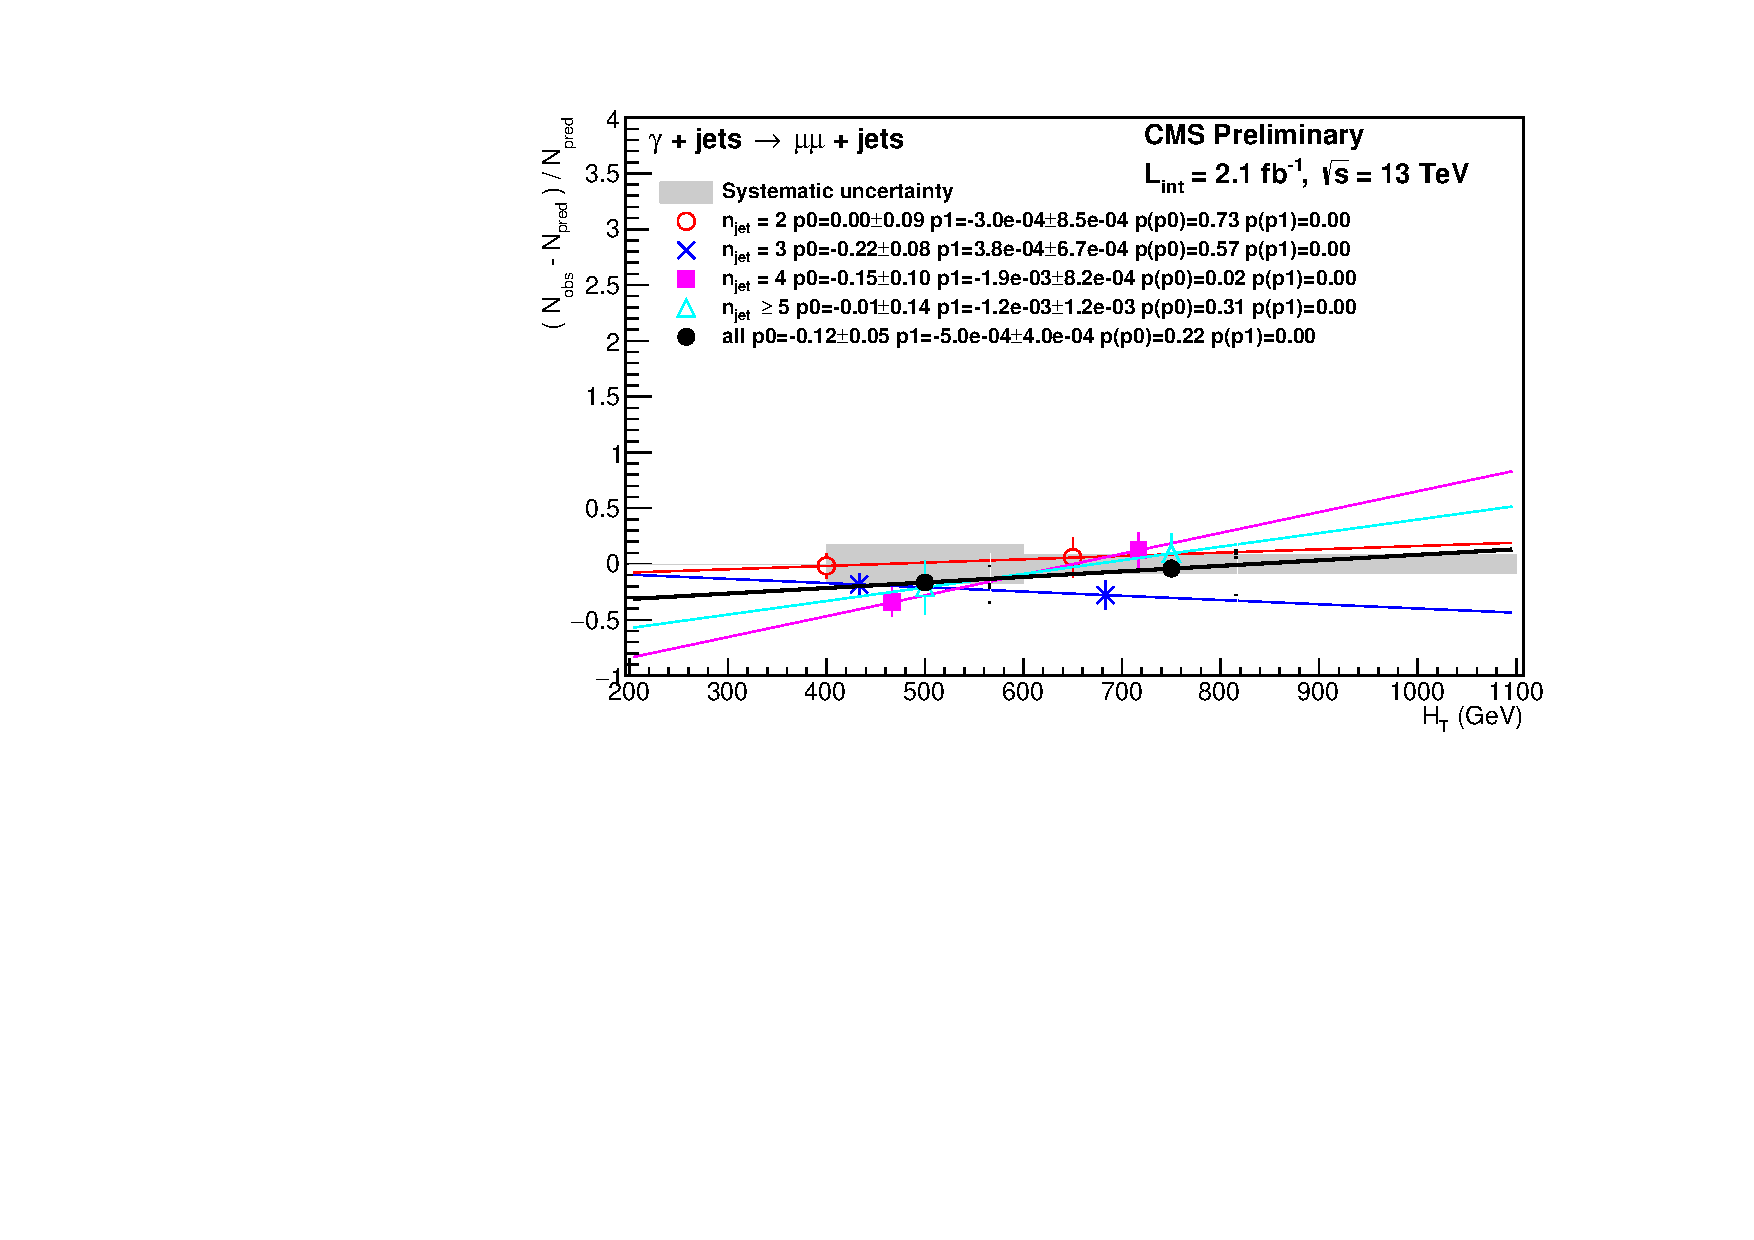
\includegraphics[width=0.45\textwidth]{figures/closureTests/phot_mumusym_half_fit.pdf}}
    ~~
    \subfigure[]{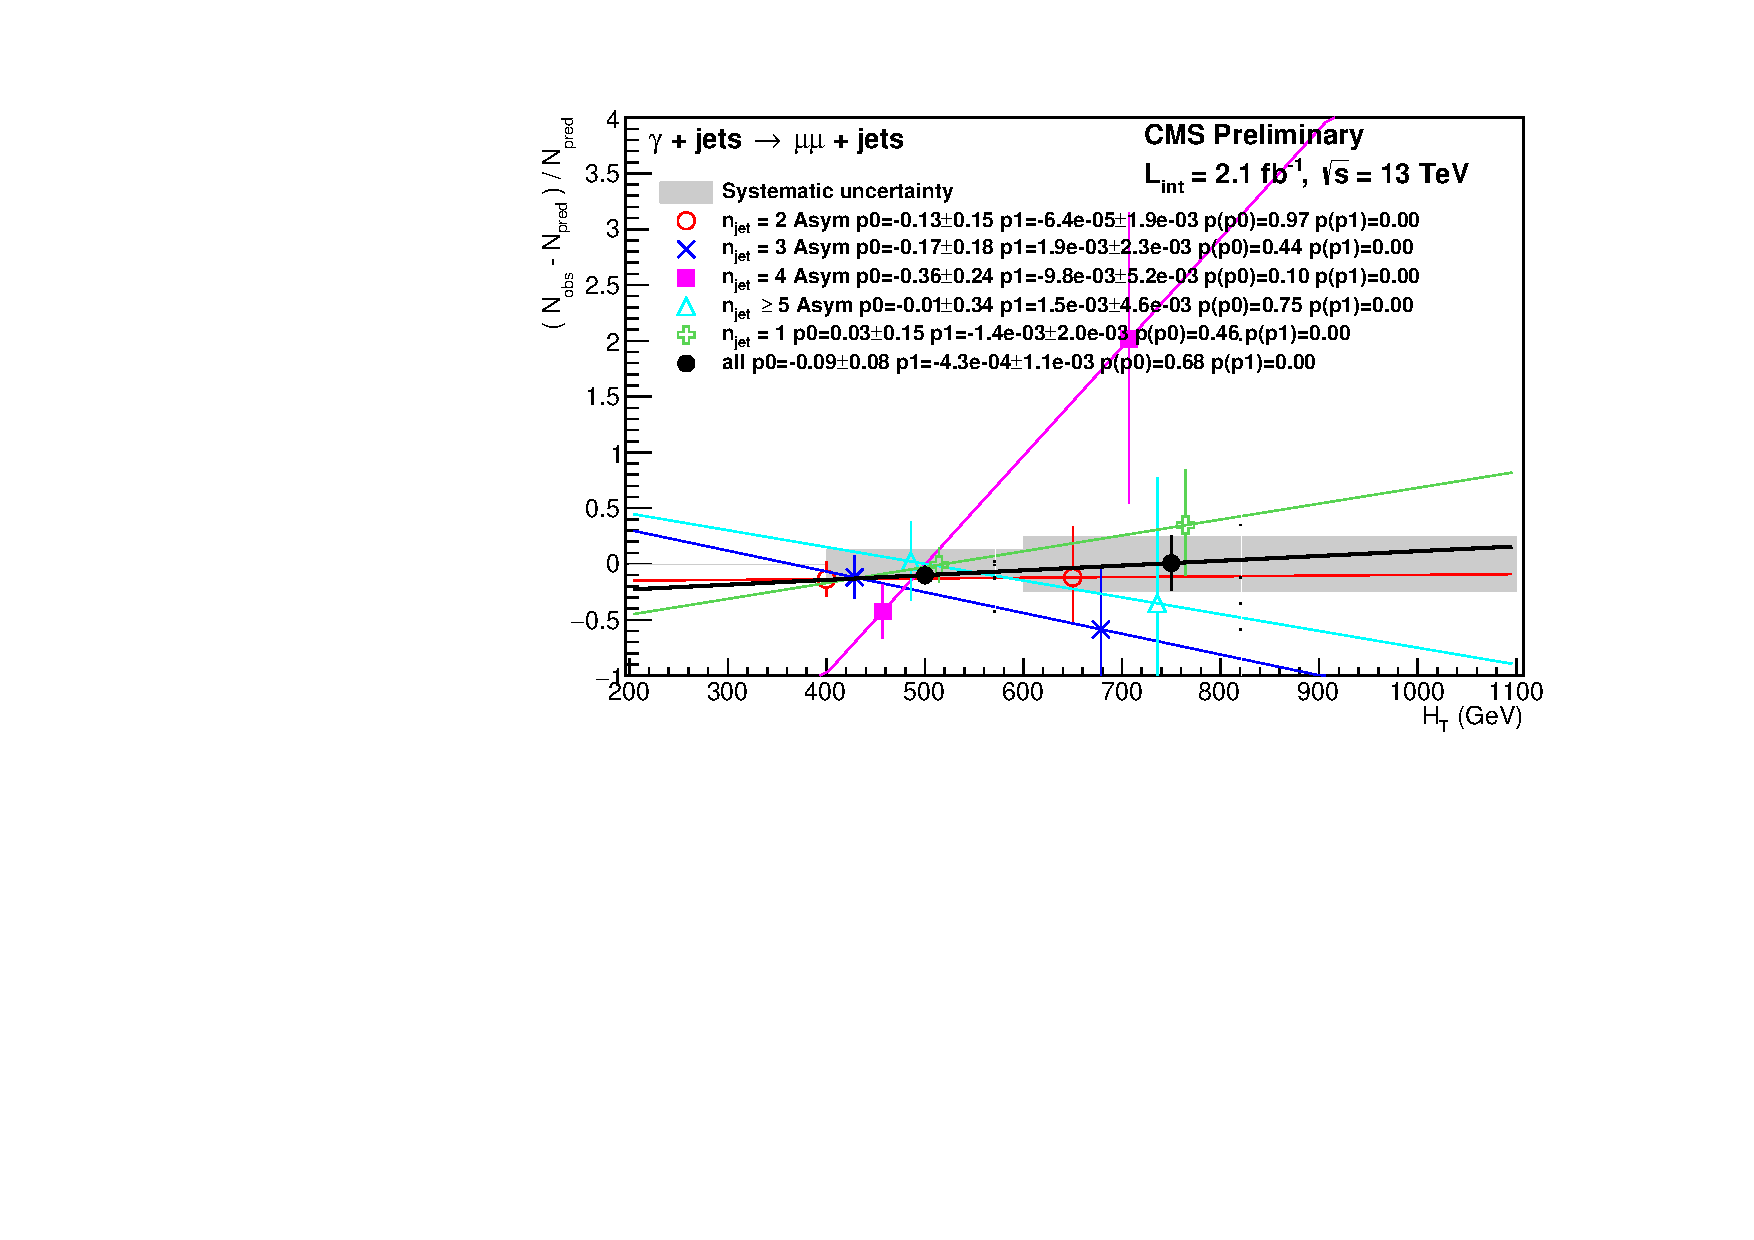
\includegraphics[width=0.45\textwidth]{figures/closureTests/phot_mumuasym_half_fit.pdf}} 
    \caption{Closure tests probing the use of the \gj control sample
      to predict the \znunu background for each
      \njet category (open symbols) overlaid on top of the systematic
      uncertainty estimates used for each of the seven \scalht bins
      (shaded bands) carried out with $2.2\ifb$ of $13\tev$
      data. The two closure tests are separated based on topology.
      Each test is fit with a linear orthogonal polynomial with the
      fit parameters on the plot.}
    \label{fig:closurePhoToMuMu}
  \end{center} 
\end{figure}

\subsection{Systematic uncertainties for the W and \ttbar background
prediction}

{\bf Variations on the transfer factors from simulation}

All the MC variations described in Sec~\ref{sec:mc-systematics} are
carried out for the transfer factors from the \mj control region to
the $W$ + jets and \ttbar background prediction. The results are shown 
in Fig.~\ref{muTtwTF}.

\begin{figure}[]
  \centering
  \subfigure[Jet energy scale varied up]{
    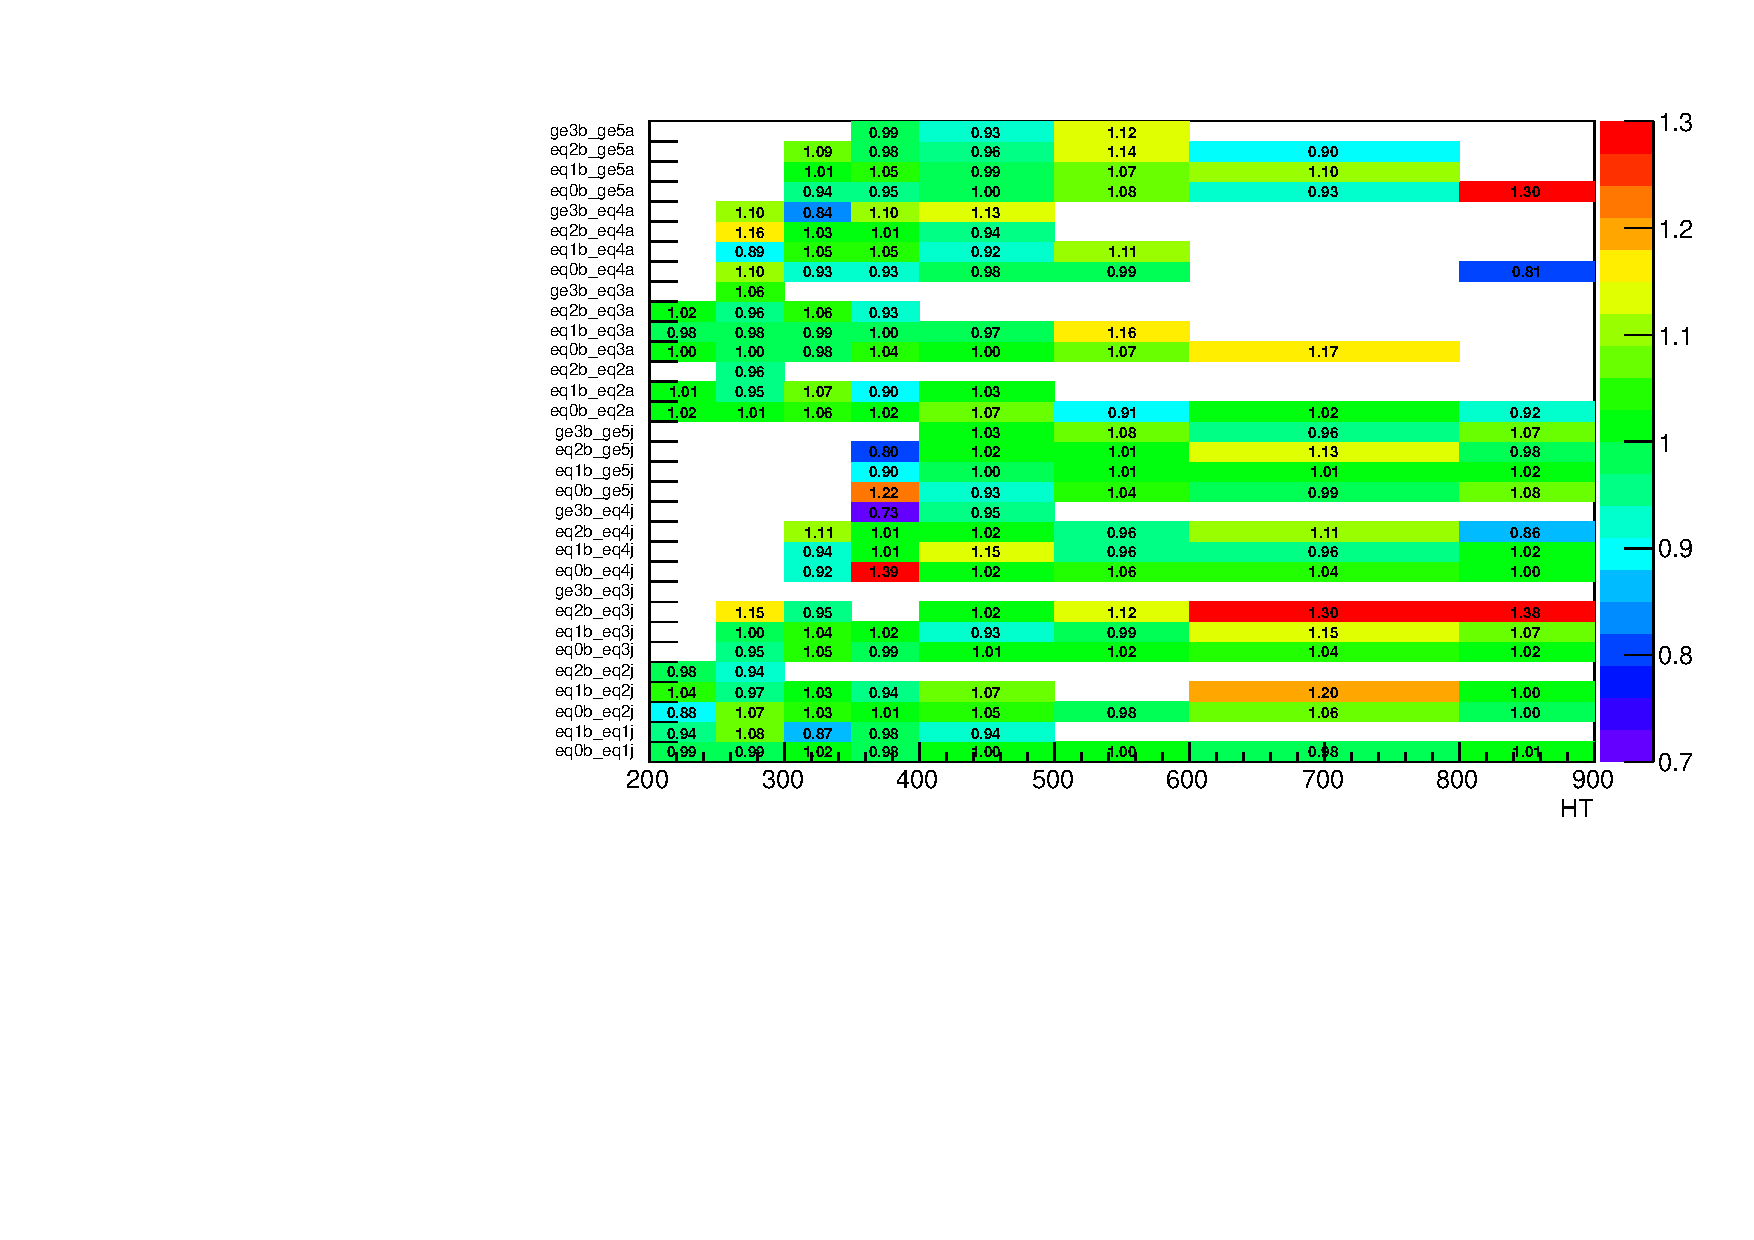
\includegraphics[width=0.5\textwidth]{figures/mcSystematics/Ttw/mu/ratiotfh_ht_mht_alljecWeight_Up.pdf}
  } ~~
  \subfigure[Jet energy scale varied down]{
    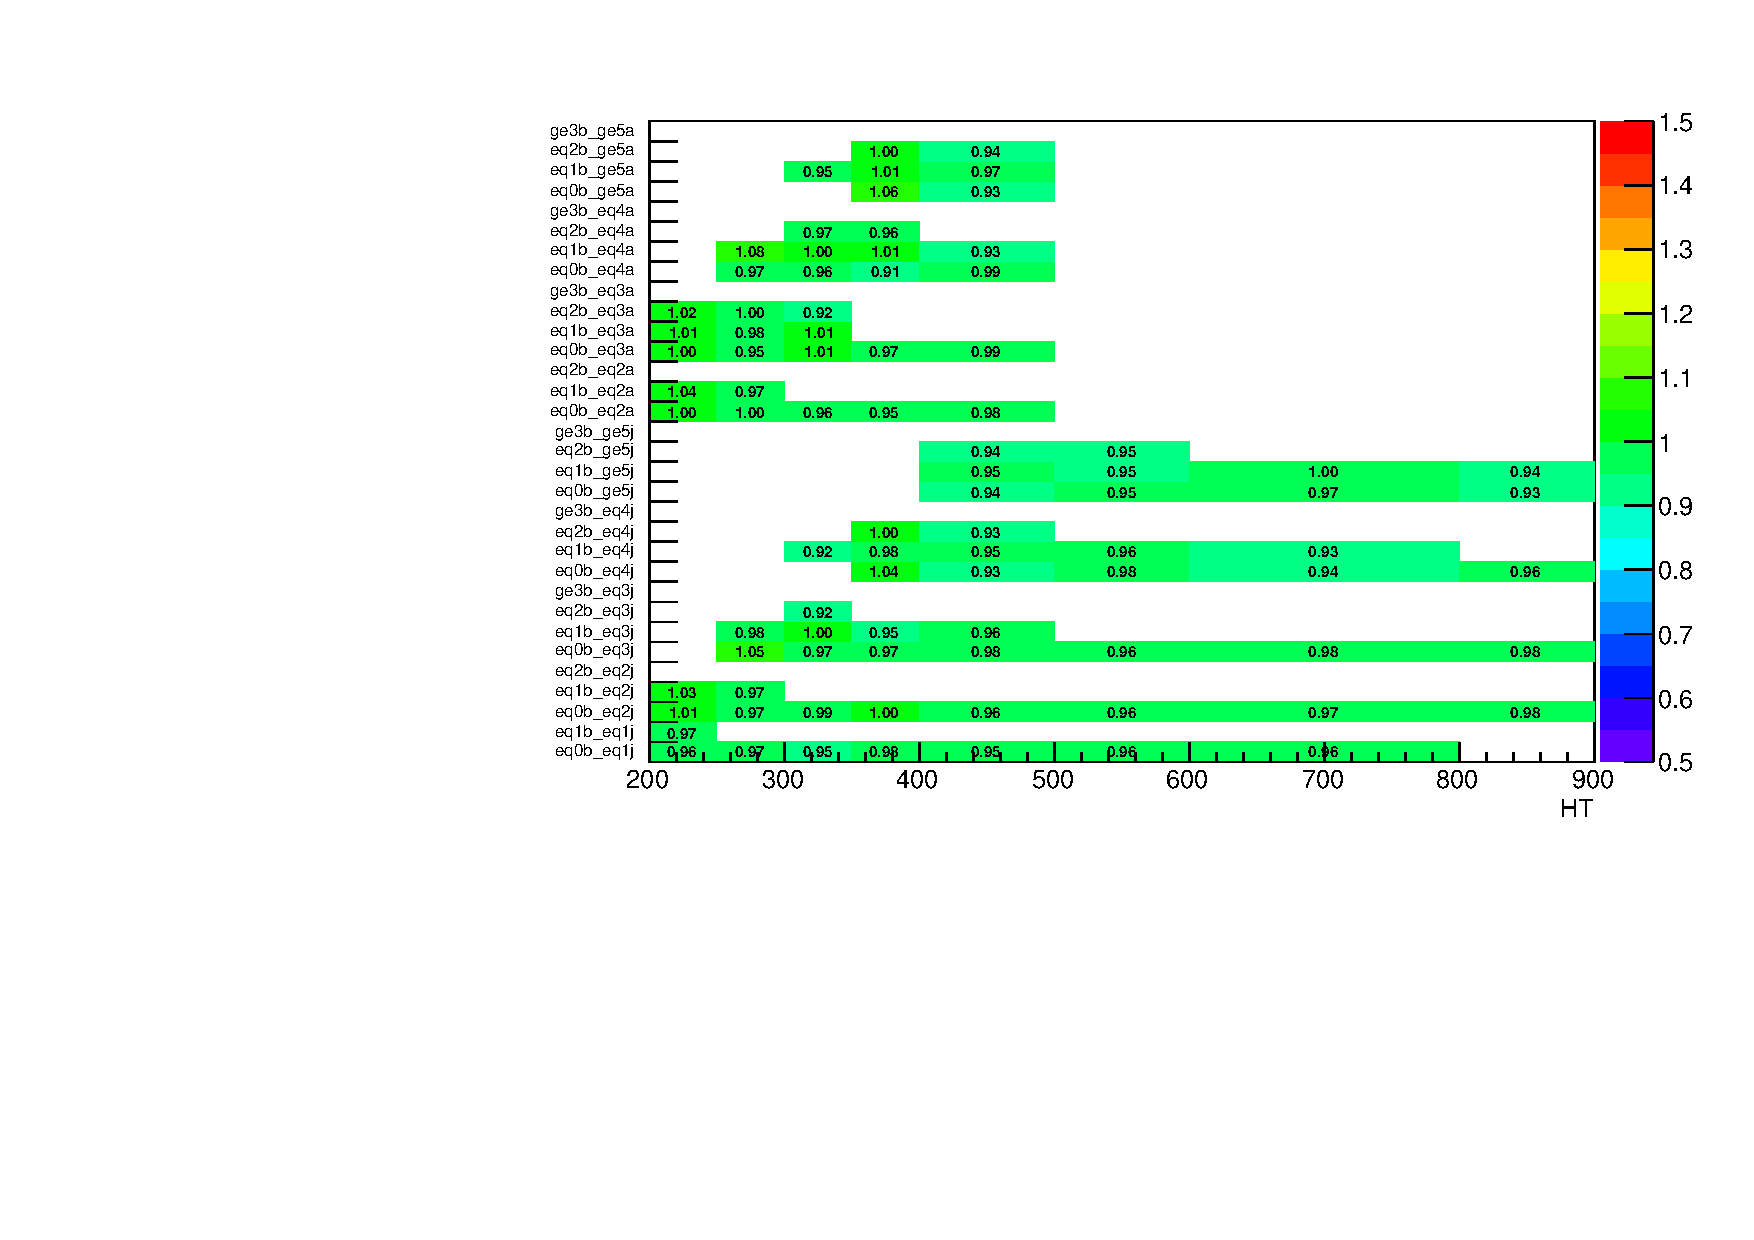
\includegraphics[width=0.5\textwidth]{figures/mcSystematics/Ttw/mu/ratiotfh_ht_mht_alljecWeight_Down.pdf}
  }\\
  \subfigure[B-tag scale factors varied up]{
    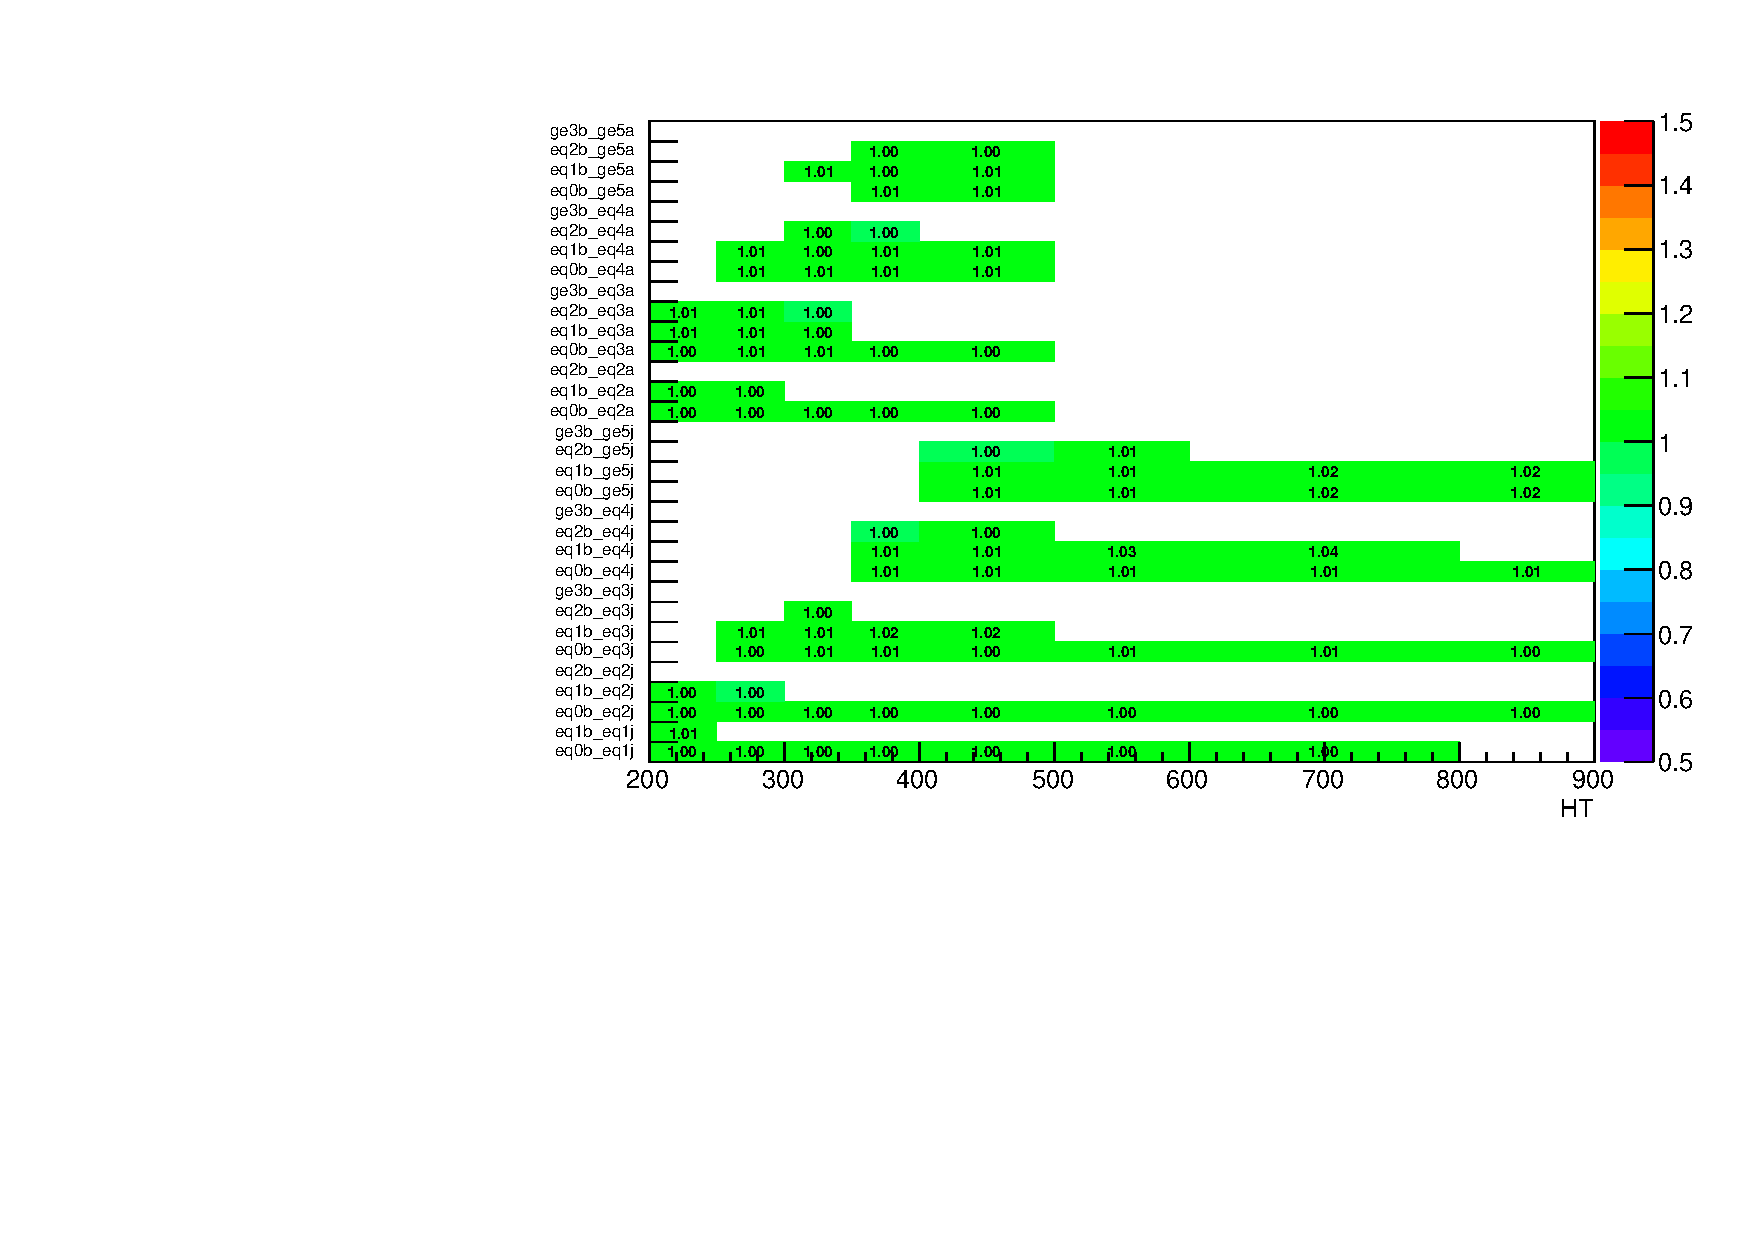
\includegraphics[width=0.5\textwidth]{figures/mcSystematics/Ttw/mu/ratiotfh_ht_mht_allbsfWeight_Up.pdf}
  } ~~
  \subfigure[B-tag scale factors varied down]{
    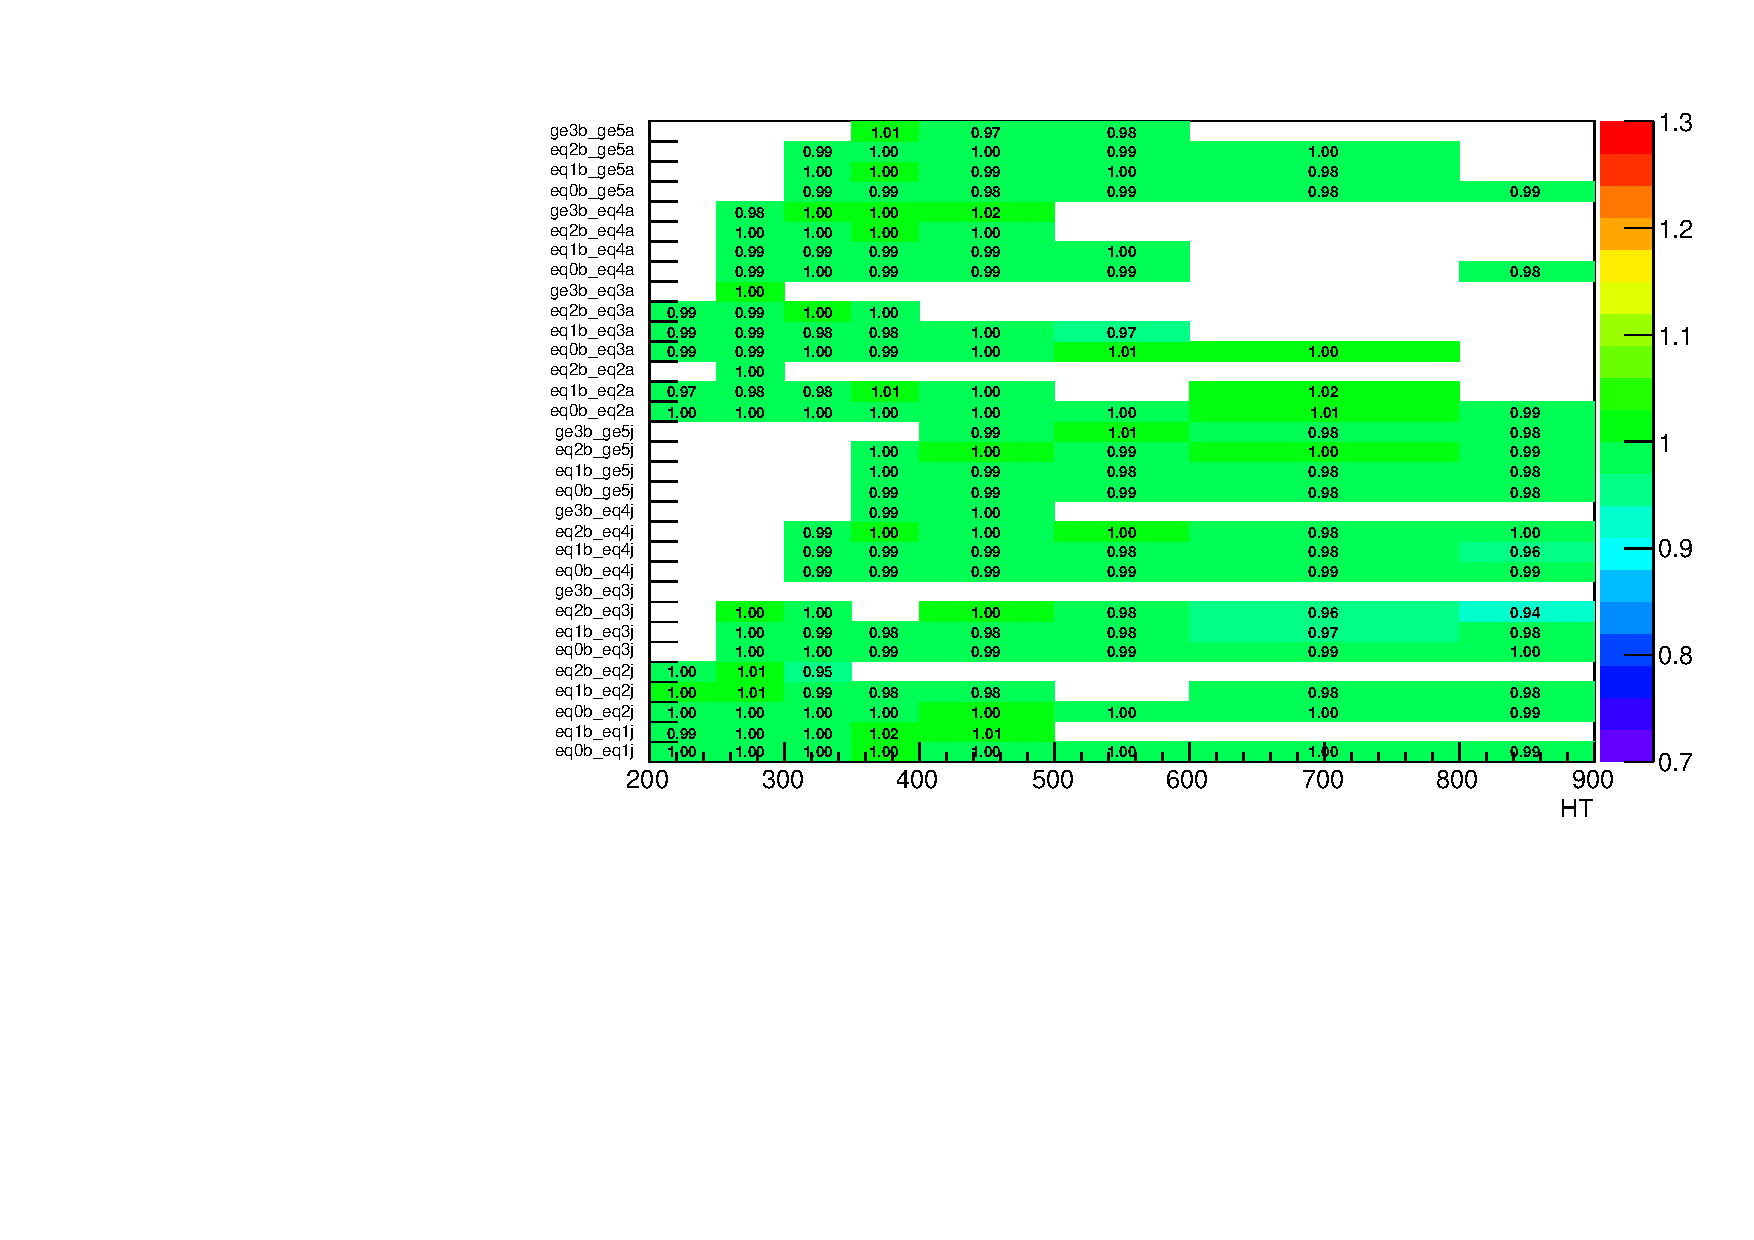
\includegraphics[width=0.5\textwidth]{figures/mcSystematics/Ttw/mu/ratiotfh_ht_mht_allbsfWeight_Down.pdf}
  }\\
  \subfigure[Pileup weights factors varied up]{
    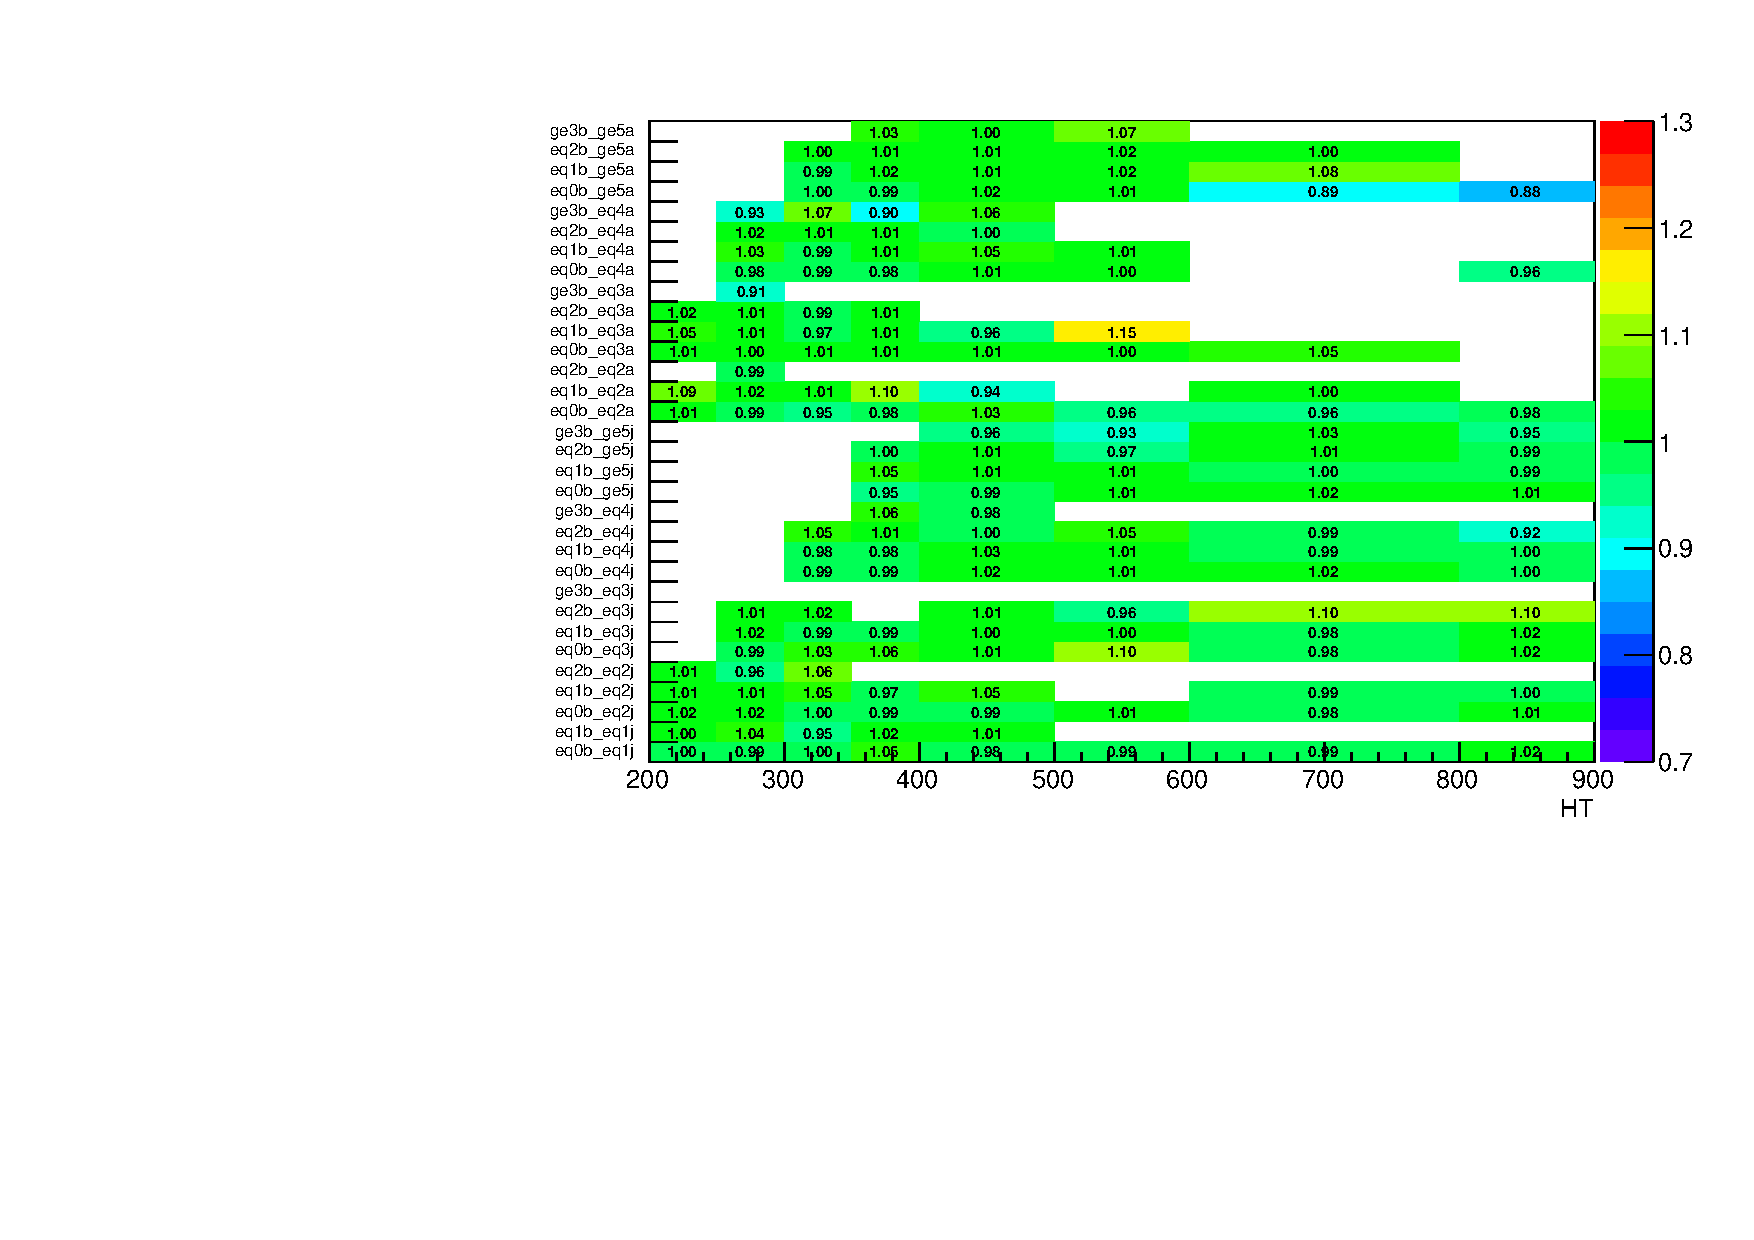
\includegraphics[width=0.5\textwidth]{figures/mcSystematics/Ttw/mu/ratiotfh_ht_mht_allpuWeight_Up.pdf}
  } ~~
  \subfigure[Pileup weights factors varied down]{
    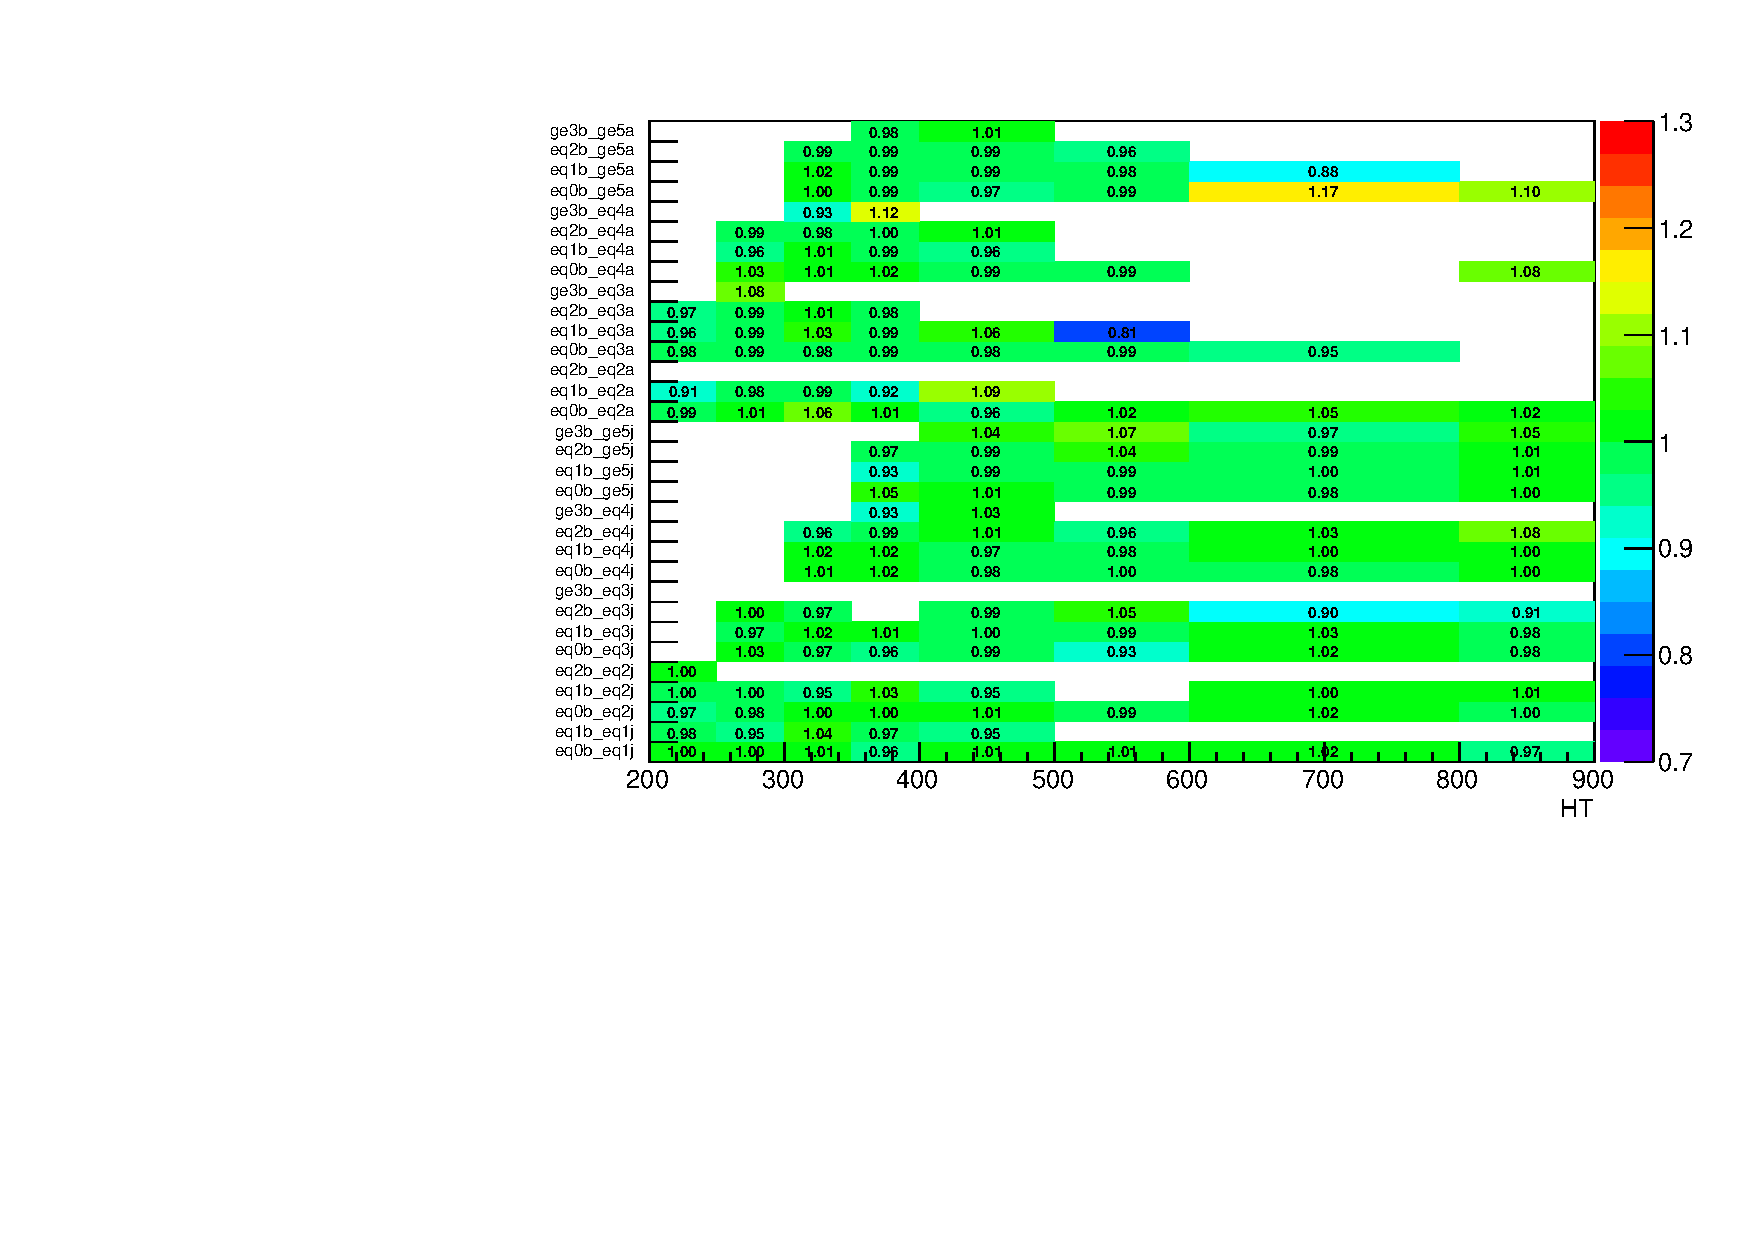
\includegraphics[width=0.5\textwidth]{figures/mcSystematics/Ttw/mu/ratiotfh_ht_mht_allpuWeight_Down.pdf}
  }\\
  \subfigure[Top $p_{T}$ weights varied up]{
    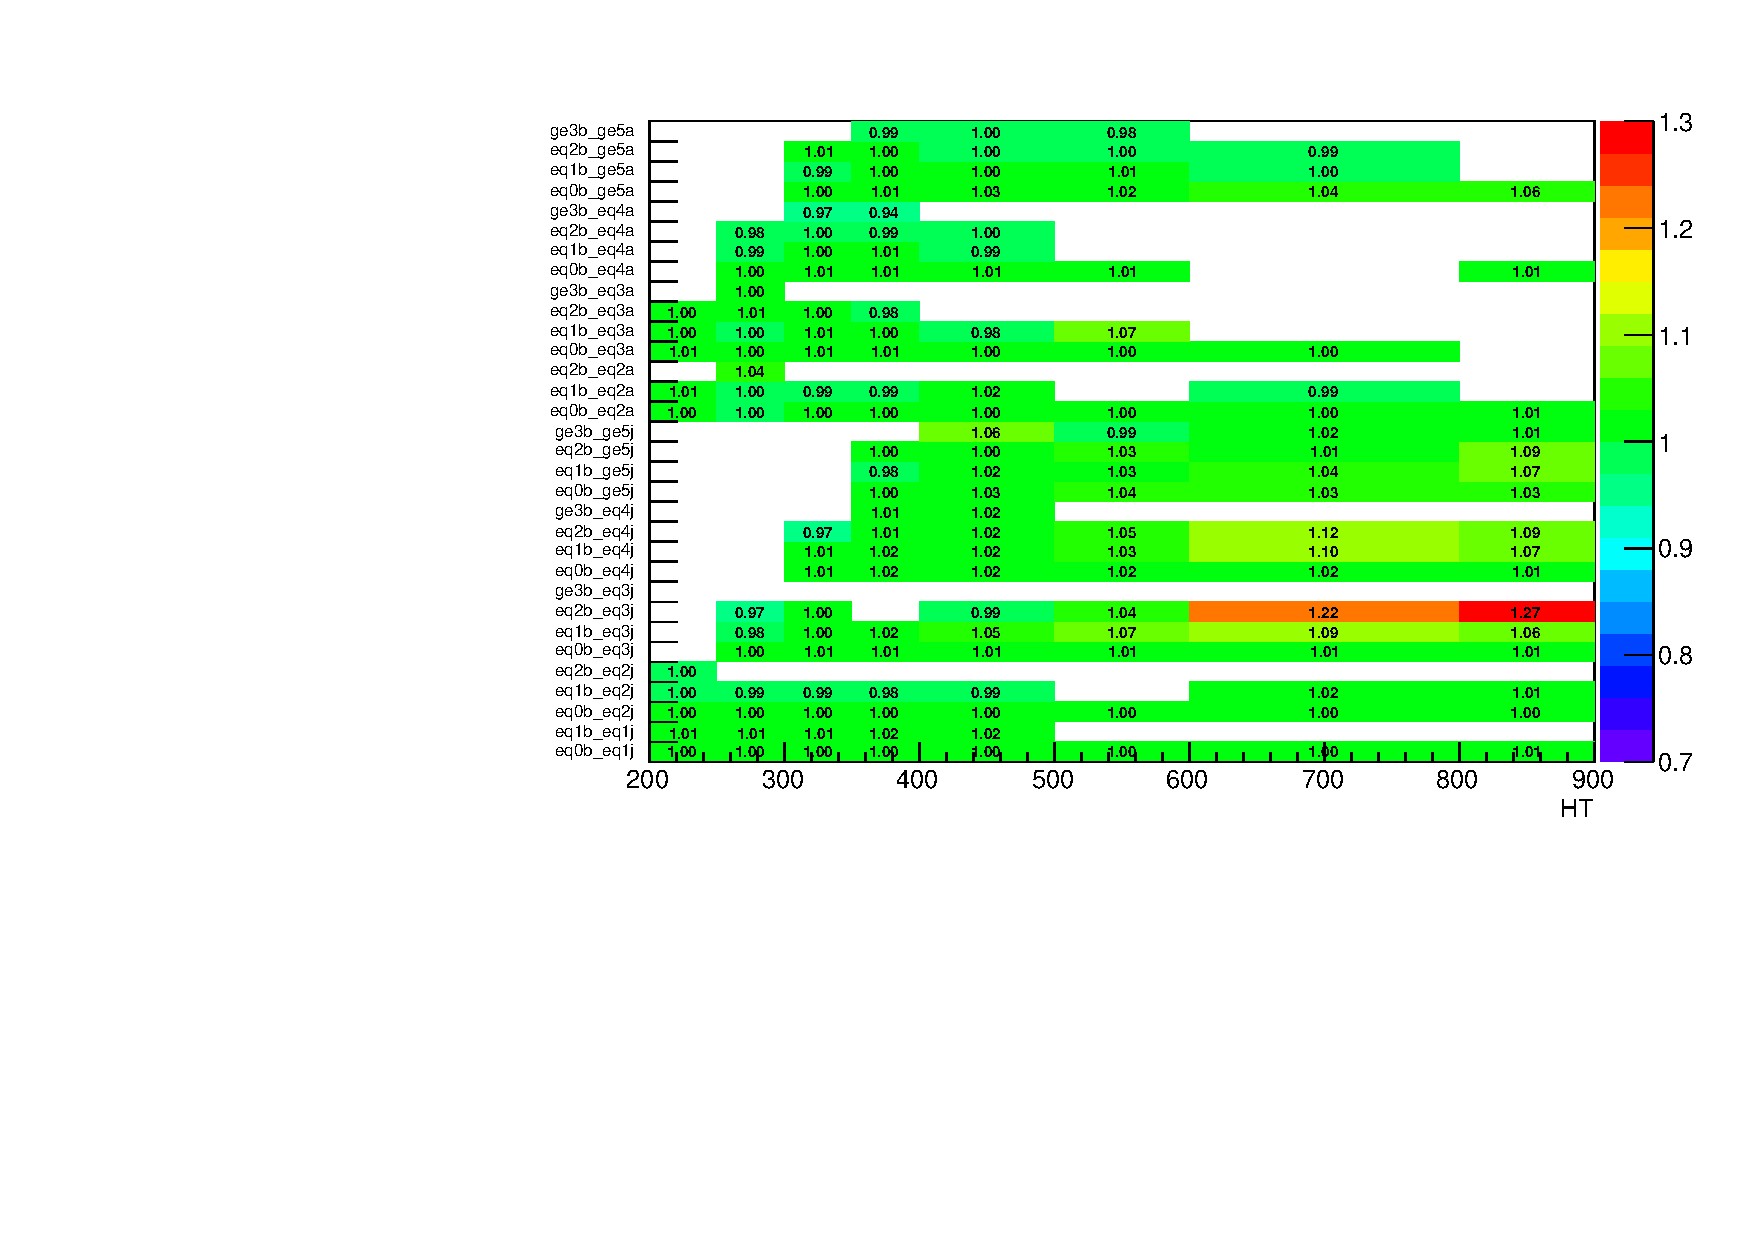
\includegraphics[width=0.5\textwidth]{figures/mcSystematics/Ttw/mu/ratiotfh_ht_mht_alltopPtWeight_Up.pdf}
  } ~~
  \subfigure[Top $p_{T}$ weights varied down]{
    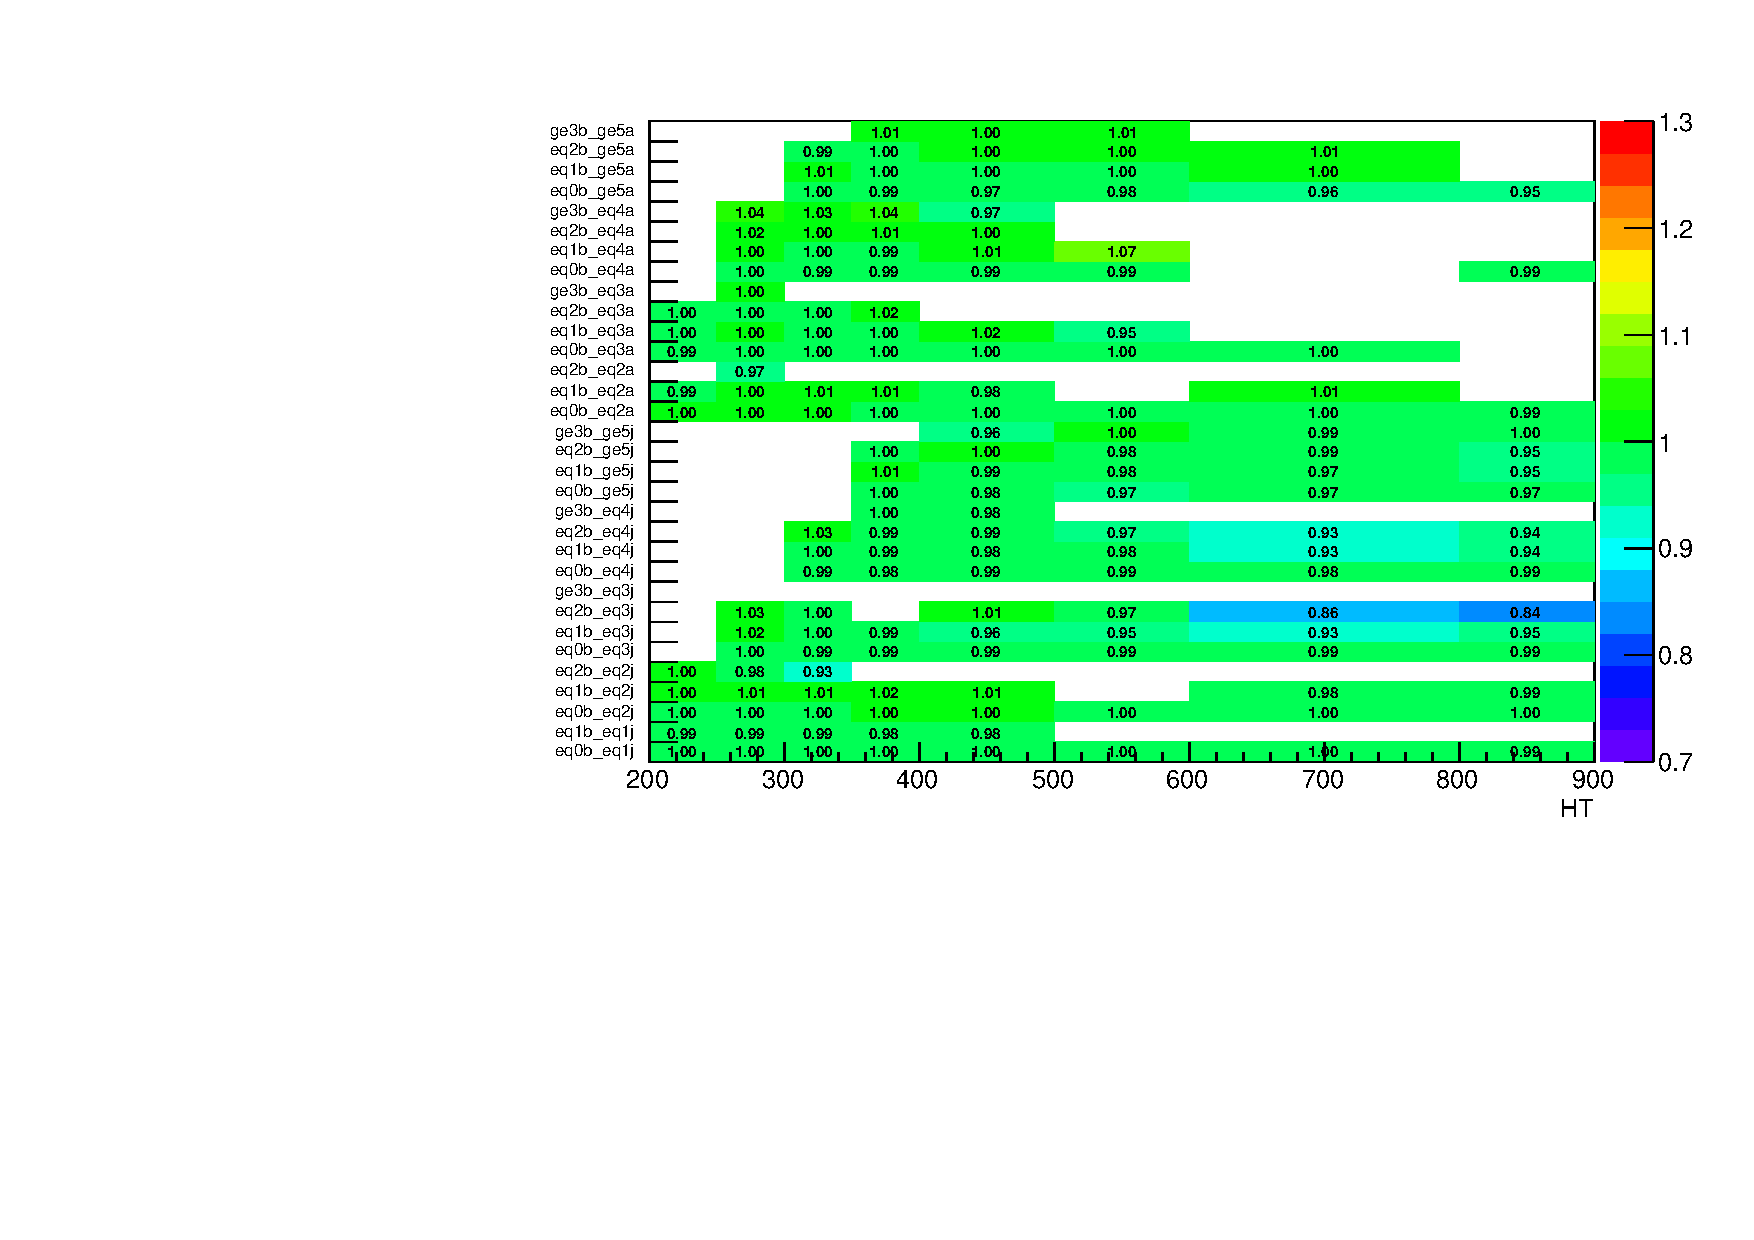
\includegraphics[width=0.5\textwidth]{figures/mcSystematics/Ttw/mu/ratiotfh_ht_mht_alltopPtWeight_Down.pdf}
  }\\
  \caption{\label{fig:muTtwTF} The change in \mj to W and \ttbar transfer
  factors when varying various parameters in the MC simulation by
  there upwards and downwards one sigma values. }
\end{figure}

{\bf Data-driven systematics}

The result of the \alphat and $\Delta\phi *$ closure tests contribute
to the systematic uncertainty as described in Sec.~\ref{sec:muZnunu}.

Additionally, the $0$ b-tag $\rightarrow1$ b-tag
tests probe the sensitivity of the transfer factors to the relative
admixture of events from the $W$ + jets and \ttbar processes by
varying the number of b-tagged jets within the \mj sample. These tests
are conservative, as the admixture changes little between the \mj
sample and the signal region (as there is no extrapolation in \nb),
whereas the closure tests use sub-samples with different \nb bins and
therefore different admixtures of $W$ + jets and \ttbar events. \eg,
the former uses a $W$-enriched sub-sample (selected by requiring zero
b-jets) to predict yields in a \ttbar-enriched sub-sample (selected by
requiring one b-jet). These tests can be seen in
Fig.~\ref{fig:closureBTag}.

The aforementioned b-tag related tests also probe the modelling of
the reconstruction of b-quark jets, although this is addressed more
precisely by dedicated studies involving varying the uncertainties in
b-tag scale factors, as the one performed in the previous analysis,
see for instance \cite{CMS_AN_2013-366}. Until the formula method is
applied, the b-tag SFs will be applied and their uncertainties
propagated through to the transfer factors.

\begin{figure}[h!]
  \begin{center}
    \subfigure[]{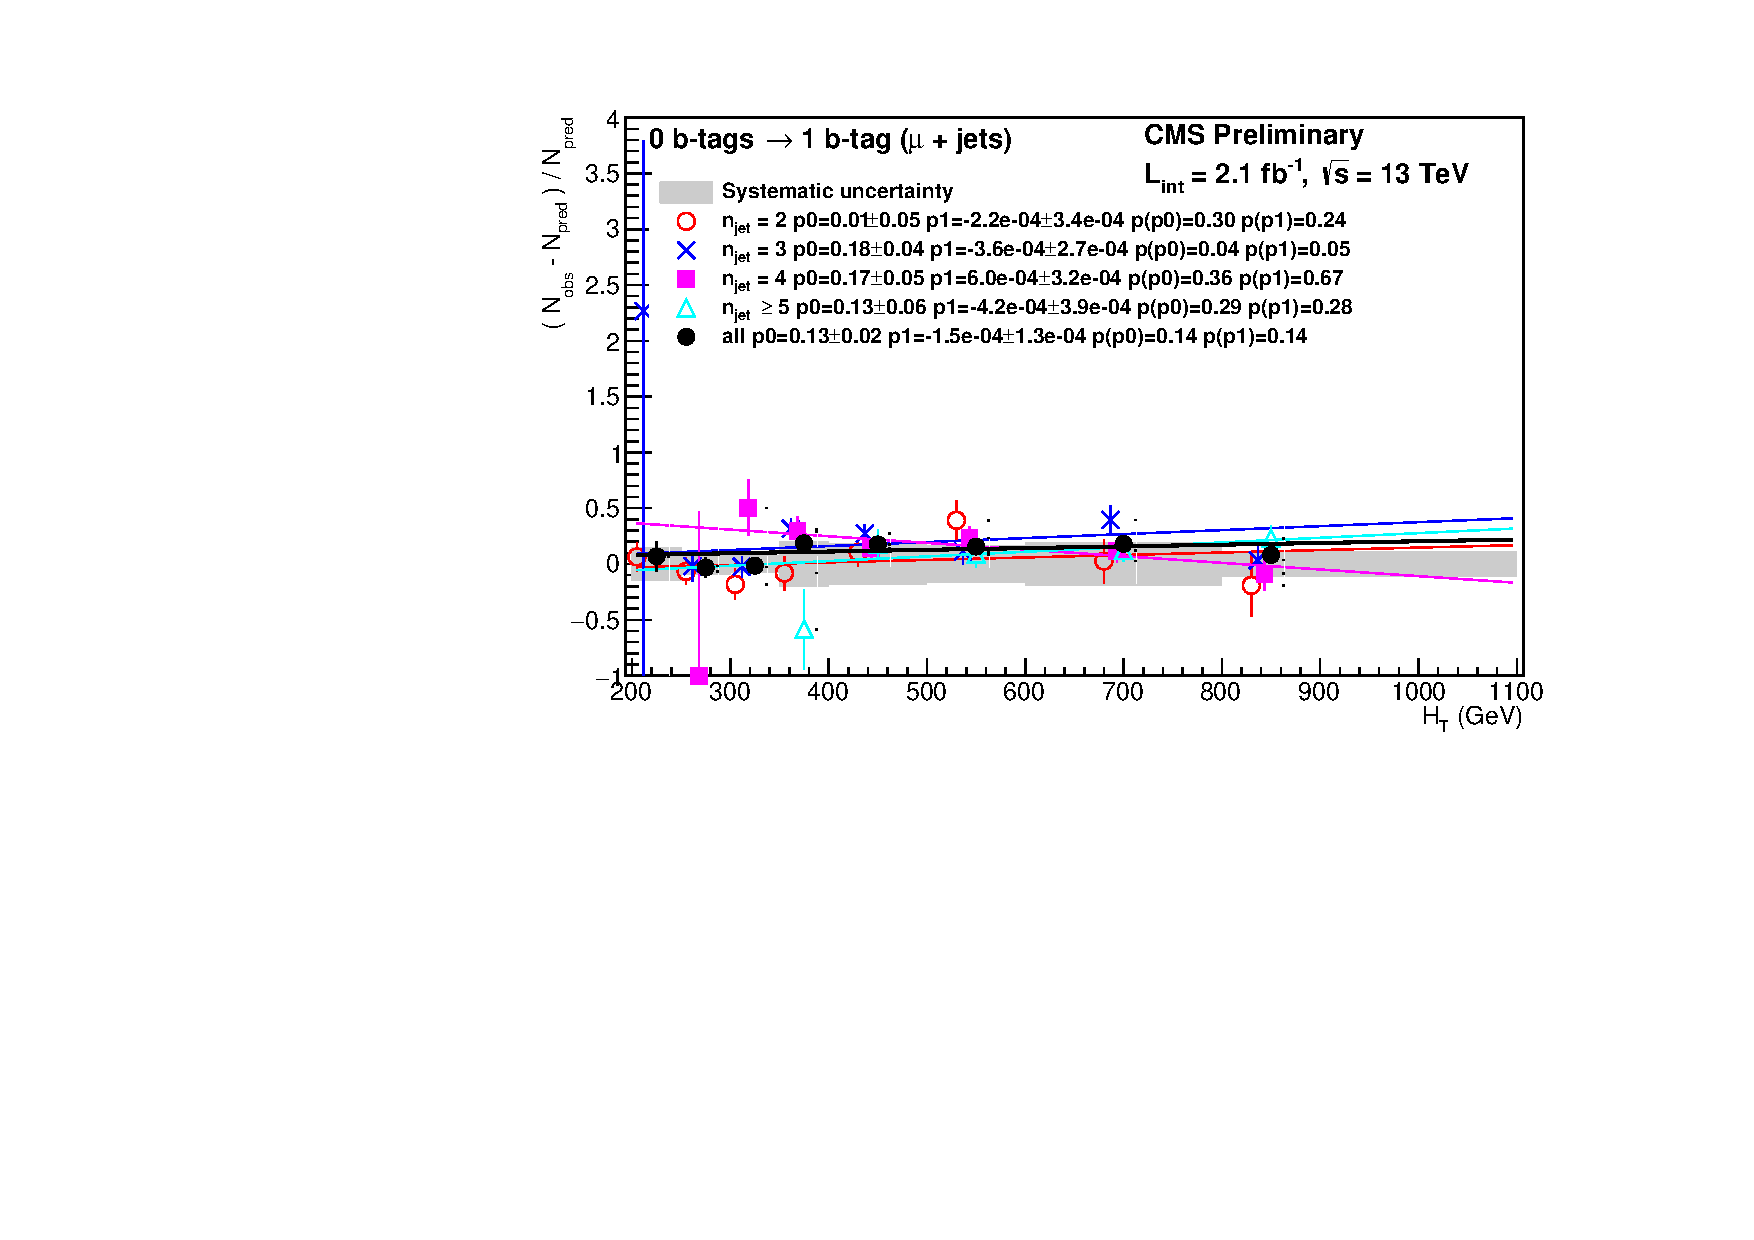
\includegraphics[width=0.45\textwidth]{figures/closureTests/eq0b_eq1b_muonsym__fit.pdf}}
    ~~
    \subfigure[]{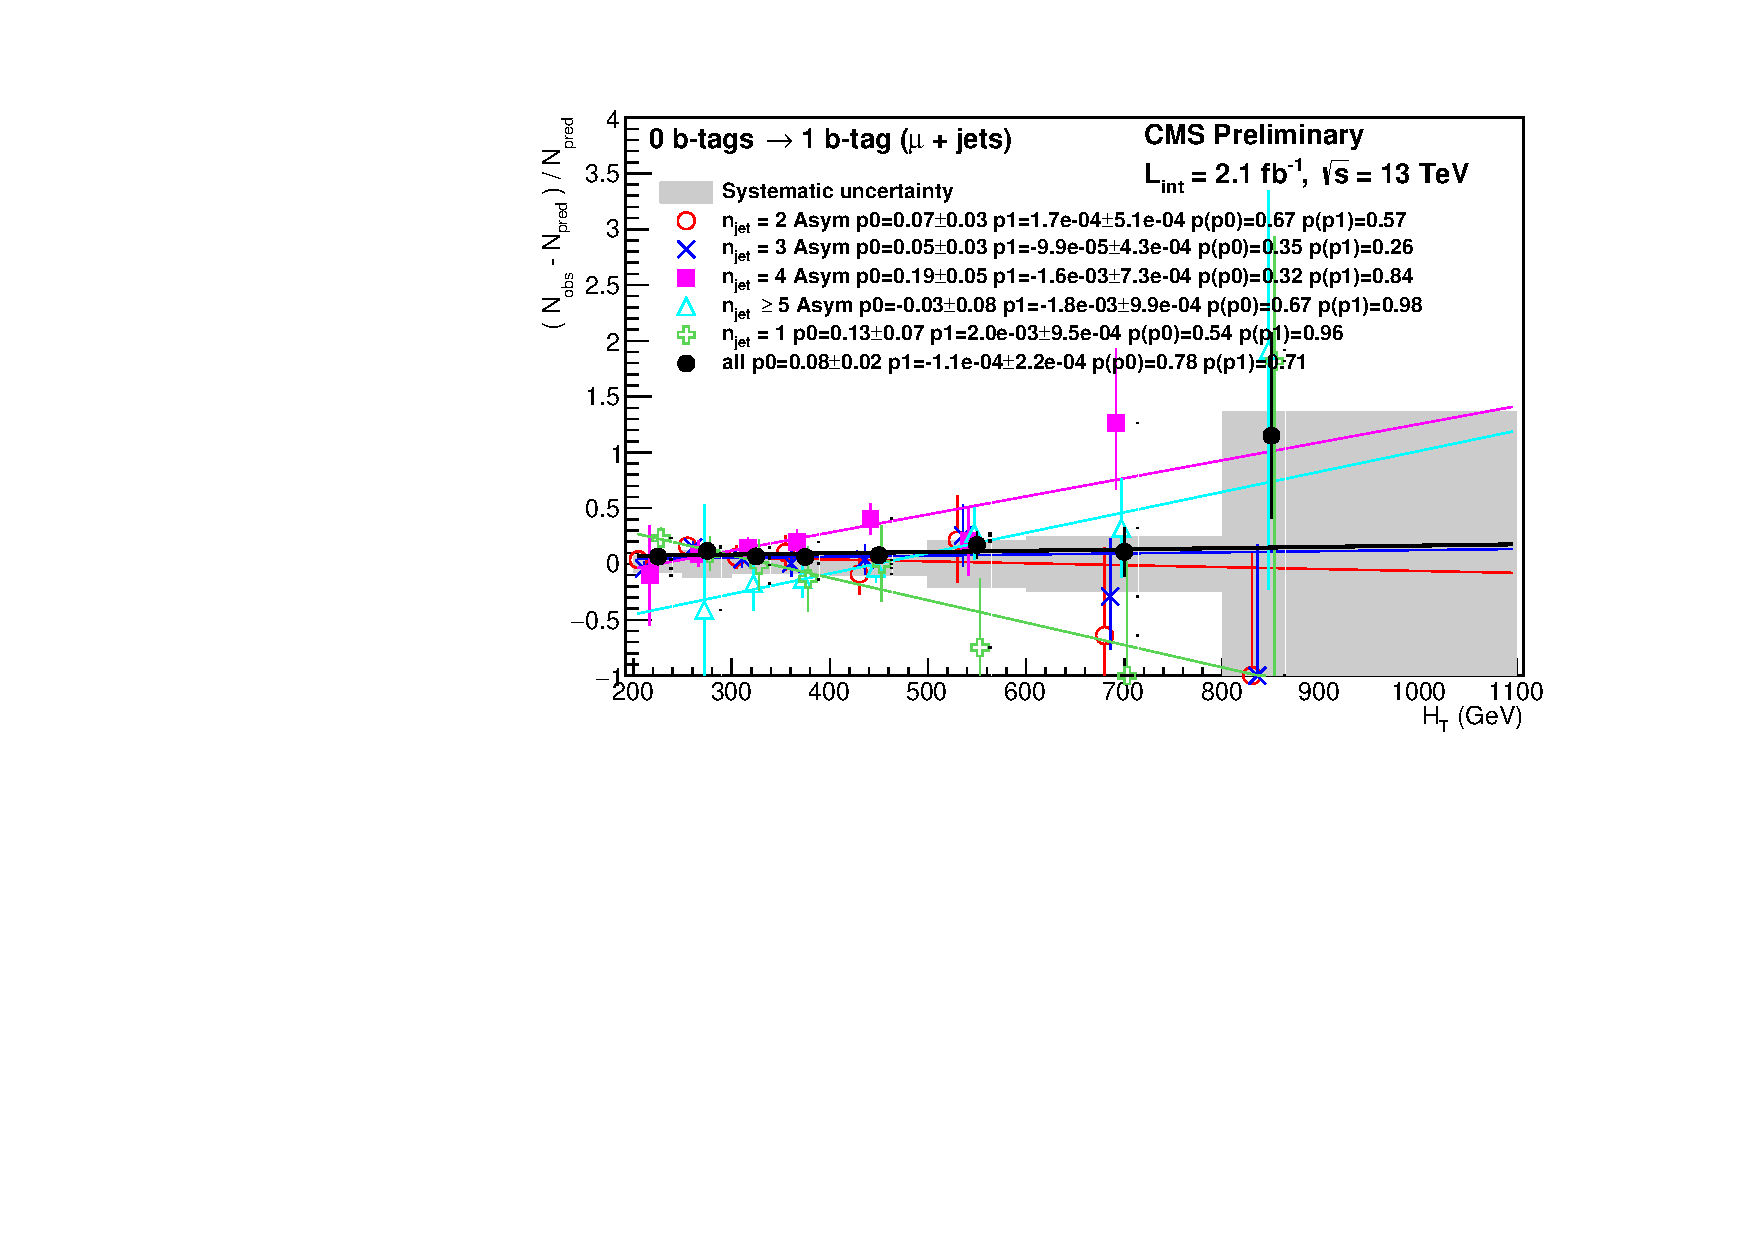
\includegraphics[width=0.45\textwidth]{figures/closureTests/eq0b_eq1b_muonasym__fit.pdf}} 
    \caption{Closure tests probing the W and \ttbar admixture through
      b-tag extrapolation are shown for each
      \njet category (open symbols) overlaid on top of the systematic
      uncertainty estimates used for each of the seven \scalht bins
      (shaded bands) carried out with $2.2\ifb$ of $13\tev$
      data. The two closure tests are separated based on topology.
      Each test is fit with a linear orthogonal polynomial with the
      fit parameters on the plot.}
    \label{fig:closureBTag}
  \end{center} 
\end{figure}

The $\mu^{+}\rightarrow\mu^{-}$ tests, as described in Sec.~\ref{sec:muZnunu} are also
considered. These ensure
that any asymmetries introduced from W polarisation effects are covered by
an appropriate systematic.

\subsubsection{Uncertainty on the lost lepton background}

Leptons out of detector 
acceptance or below the $p_{T}$ threshold, or leptons within detector
acceptance but not idenfitied properly by lepton ID or isolation
requirements lead to a W and \ttbar lost lepton background. The
fraction of events with leptons out of acceptance ($f_{sample}$)
is calculated from generator truth level information for each MC
sample. Differences in efficiencies between data and simulation are
accounted for with POG provided lepton scale
factors for lepton ID and isolation~\cite{twiki-leptonSF}. The
uncertainties on the transfer factors associated 
with these scale factors are determined by varying each of them by
their associated errors.

The lost lepton background contribution for each category (\njet, \nb, \scalht), to 
transfer factors is summarised as:
\begin{equation}
    \label{eq:lostLepTF}
    y = \frac{\sum_{sample} [ R_{sample} \times f_{sample} \times N^{GEN}_{sample} \times ( 1 - \epsilon_{Loose} ) + ( 1 - f_{sample} ) \times N^{GEN}_{sample} ]}{ \sum_{sample} N^{GEN}_{sample} \times \epsilon_{Tight} \times R_{sample} }
\end{equation}
where $R_{sample}$ is the cross section reweighting factor for each sample, 
$N^{GEN}_{sample}$ is the total MC events for the category, $\epsilon_{Tight}$
and $\epsilon_{Loose}$ are the lepton efficiency for Tight and Loose working 
point. The variable $y$ is computed for each category. For the numerator, full
signal selection except the lepton veto to mimic signal region phase space as
closely as possible. For the denominator, the full selection for \mj + jets 
control sample is applied.

The variation on the variable $y$ is computed by varying the lepton scale factor
up and down according to each systematic and statistic uncertainty from lepton
ID and isolation, according to the POG recommendation. Then the up and down 
variations are added in quadrature respectively, to give an overall systematic 
uncertainty. The procedure is repeated separately for muon and electron.

\begin{figure}[]
  \centering
  \subfigure[Muon scale factors varied up]{
    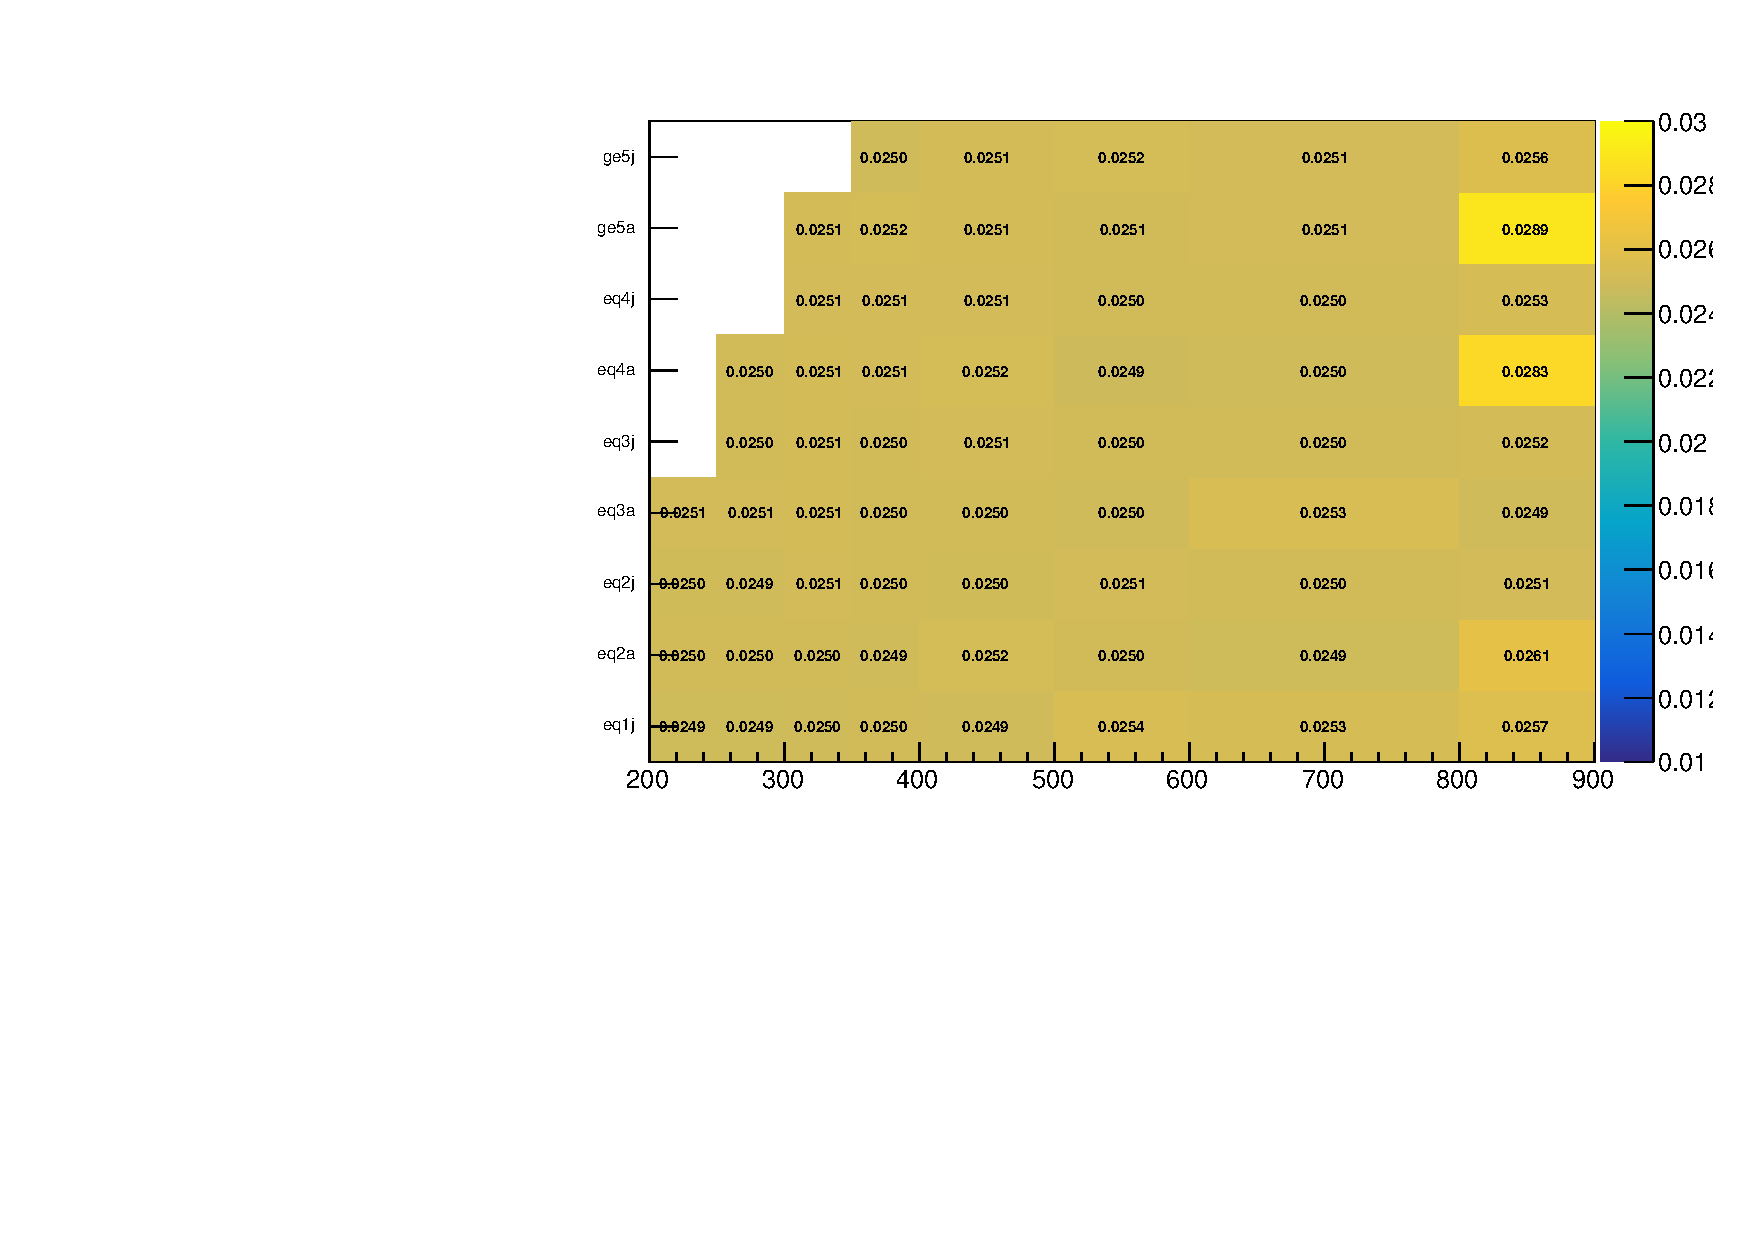
\includegraphics[width=0.5\textwidth]{figures/mcSystematics/lostLepton/muonUp.pdf}
  } ~~
  \subfigure[Muon scale factors varied down]{
    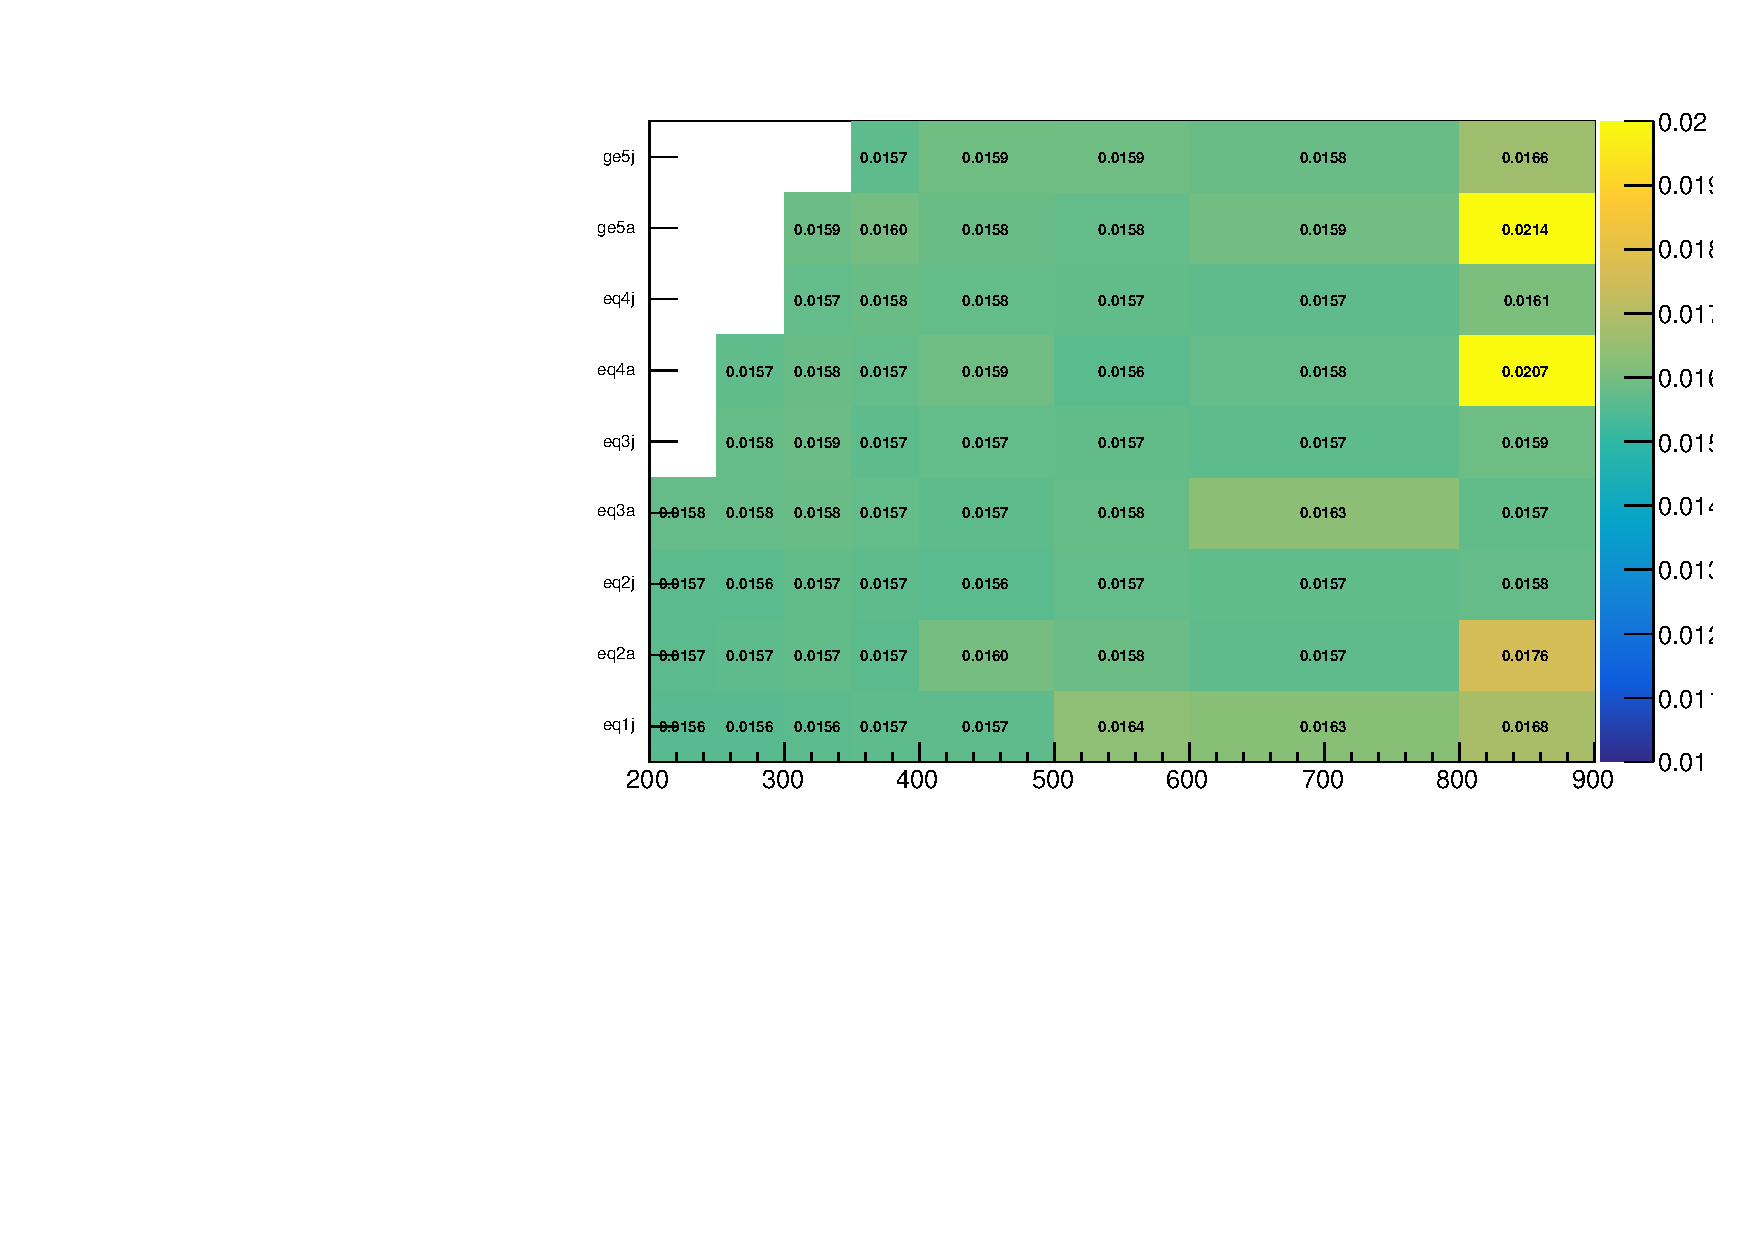
\includegraphics[width=0.5\textwidth]{figures/mcSystematics/lostLepton/muonDown.pdf}
  }\\
  \subfigure[Electron scale factors varied up]{
    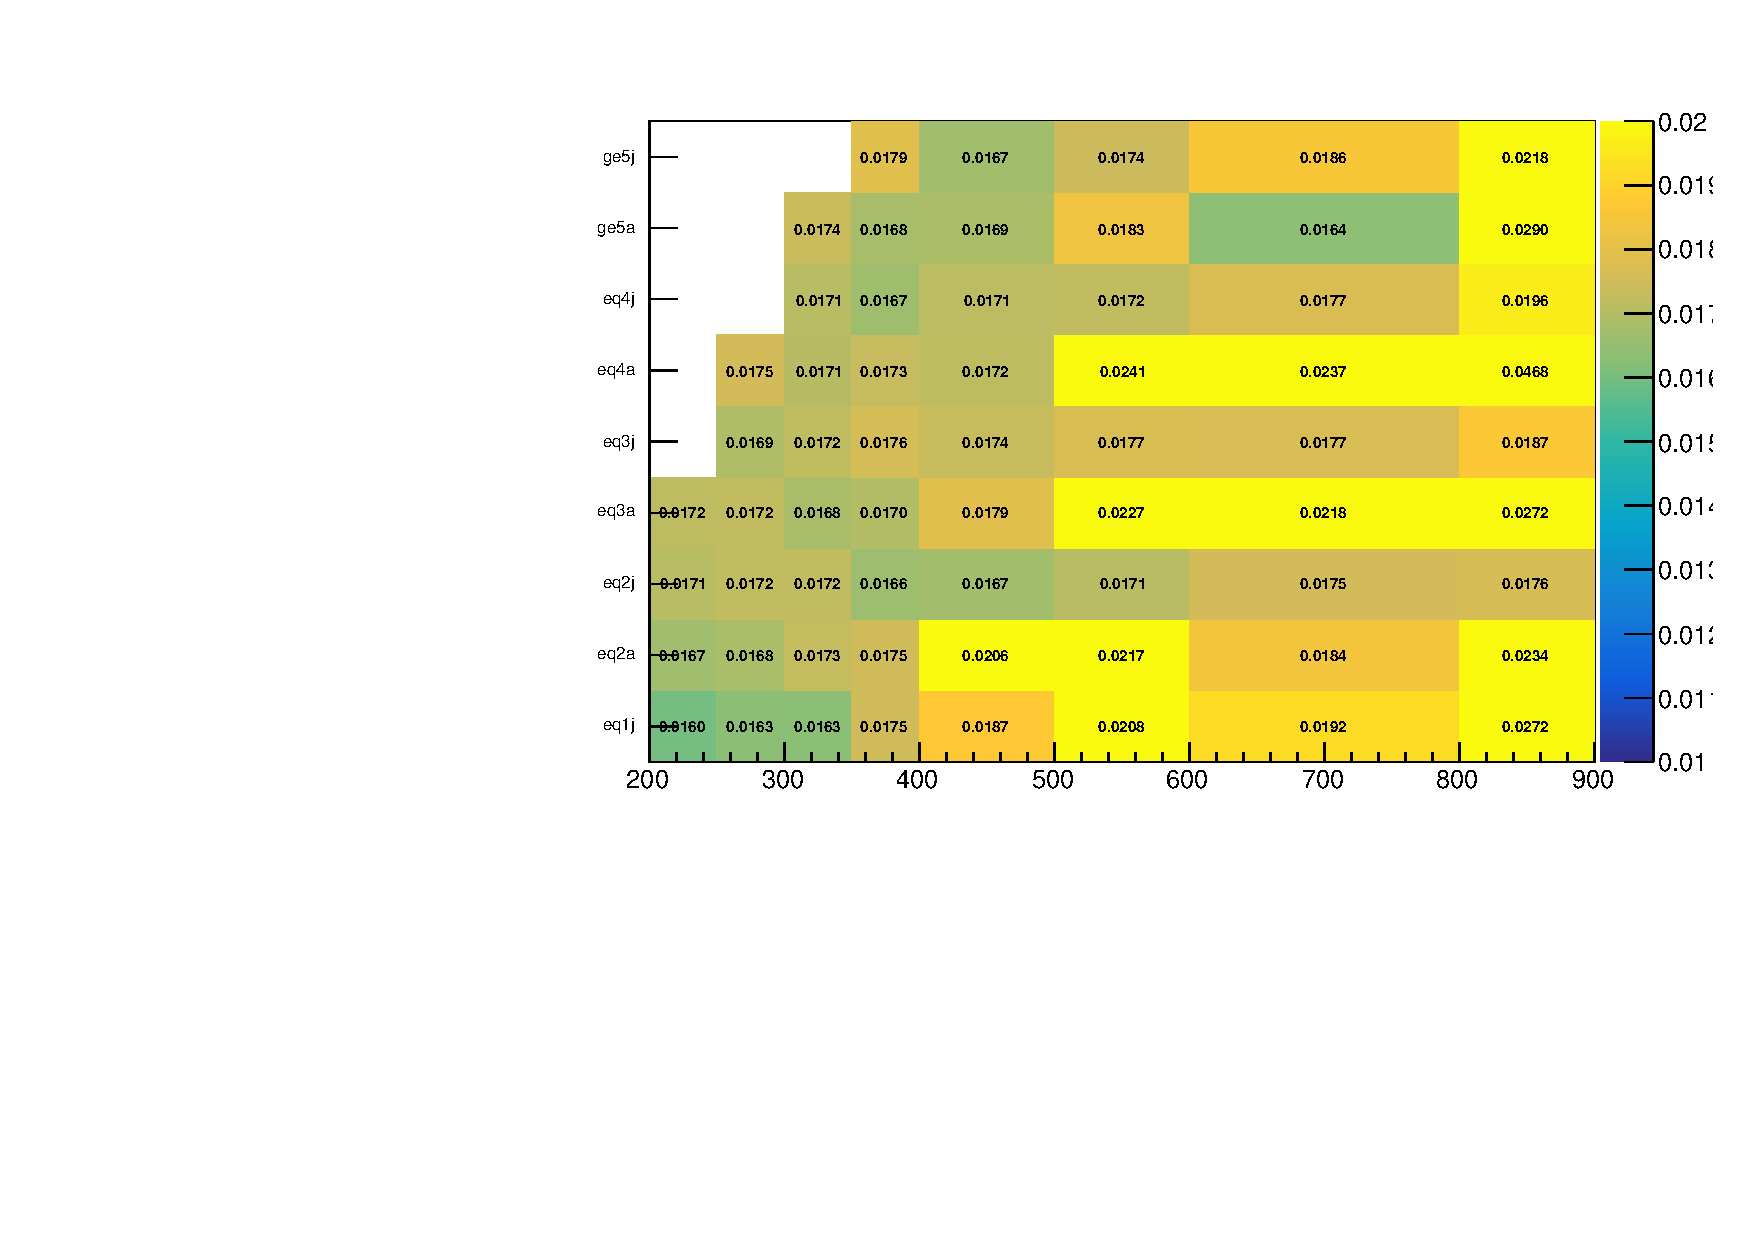
\includegraphics[width=0.5\textwidth]{figures/mcSystematics/lostLepton/electronUp.pdf}
  } ~~
  \subfigure[Electron scale factors varied down]{
    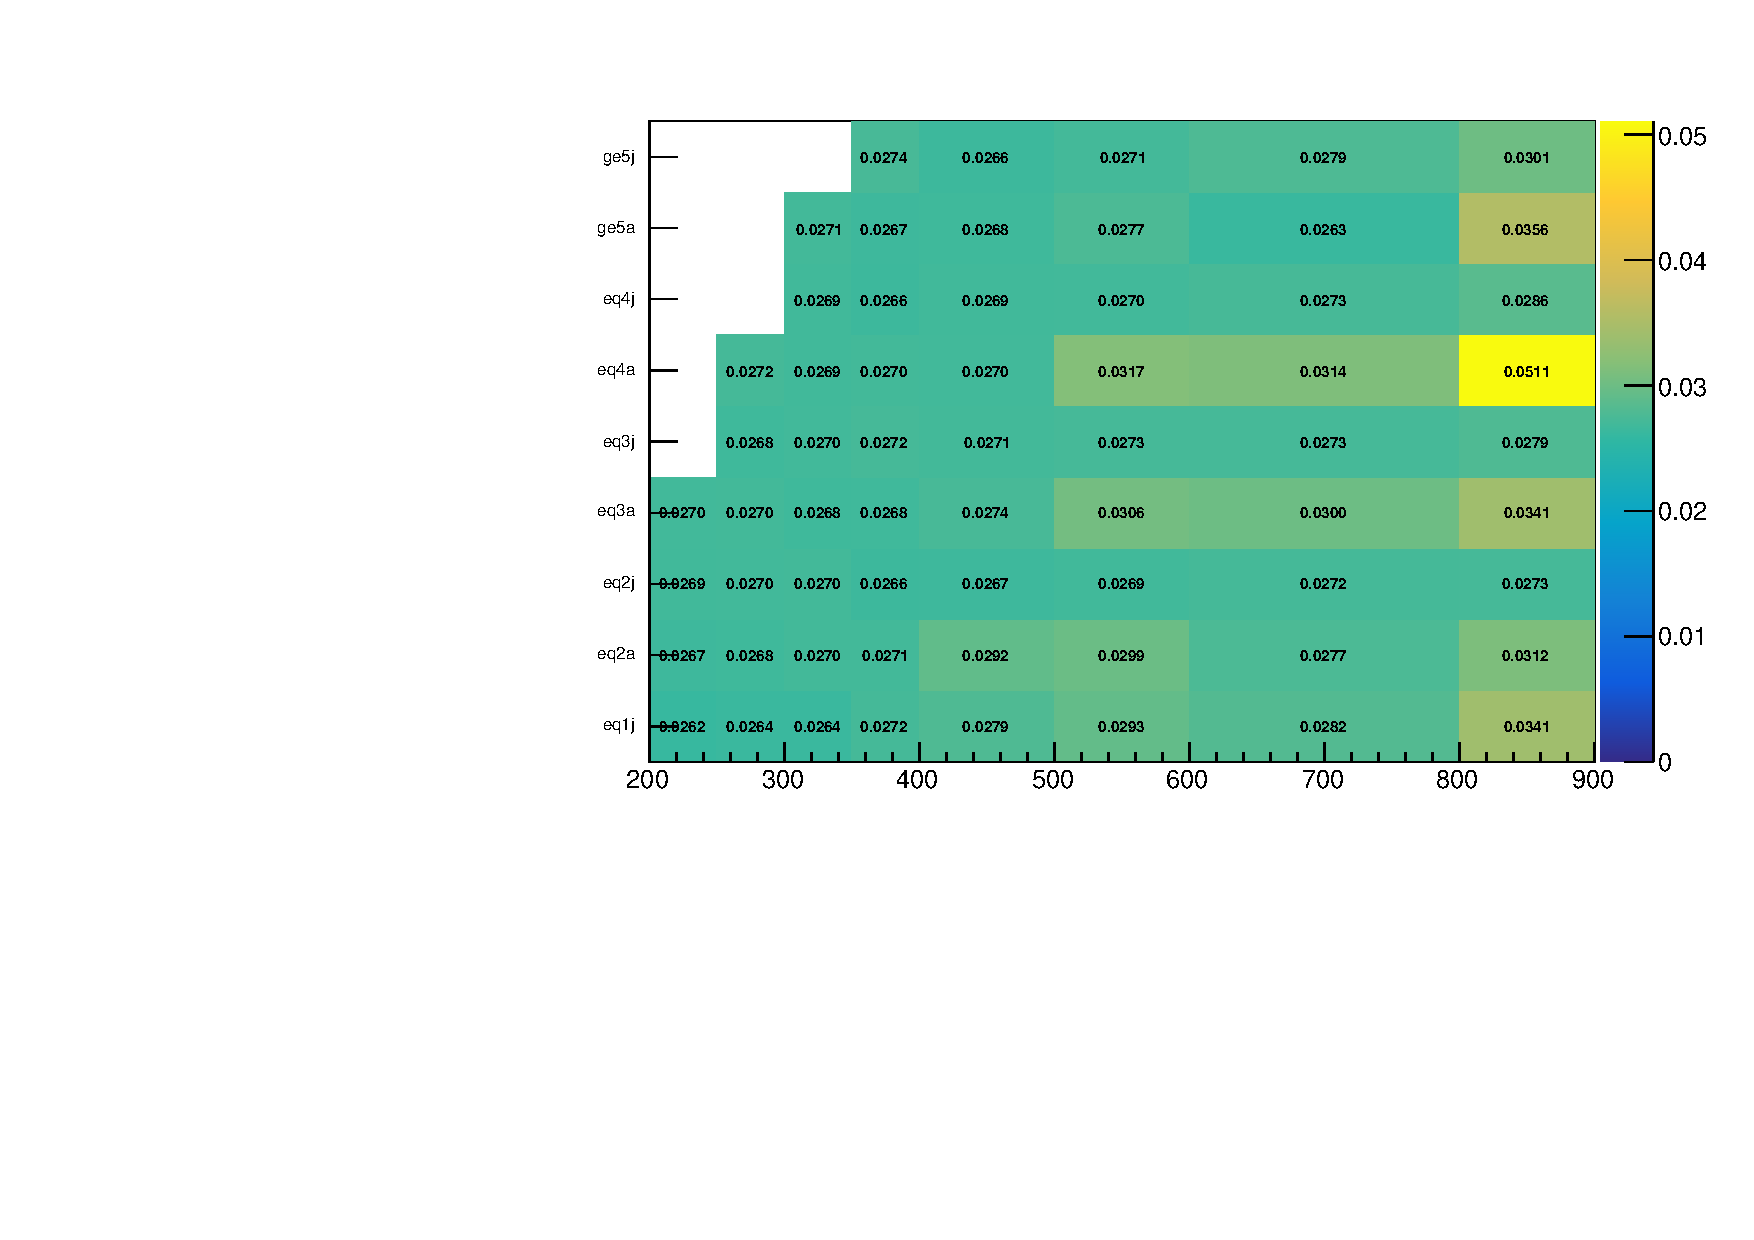
\includegraphics[width=0.5\textwidth]{figures/mcSystematics/lostLepton/electronDown.pdf}
  }\\
  \caption{\label{fig:lostLepton} The upwards and downwards variations on the variable $y$
  from the muon and electron lepton scale factors. This is used as a
  systematic uncertainty on the \mj to W and \ttbar
  transfer factor. }

\end{figure}

% \subsection{Additional closure tests as cross checks}
% \label{sec:closureCrossCheck}
%
% Along with the closure tests used to derive the systematics,
% additional tests are carried out to cross check other potential
% instances of mismodelling. If any of these tests demonstrate a source
% of bias, further investigation into this effect is carried out. 
%
% The closure tests in Fig.~\ref{fig:closureLooseLep} probe the effects
% of the extrapolation in the lepton definition used for the veto in the
% signal region, as described in Sec.~\ref{sec:closure-tests-data}.
% These tests are included in the systematic calculation for the W and
% \ttbar + jets backgrounds, but can be seen in isolation here. 
%
% \begin{figure}
%   \begin{center}
%     \subfigure[Closure tests]{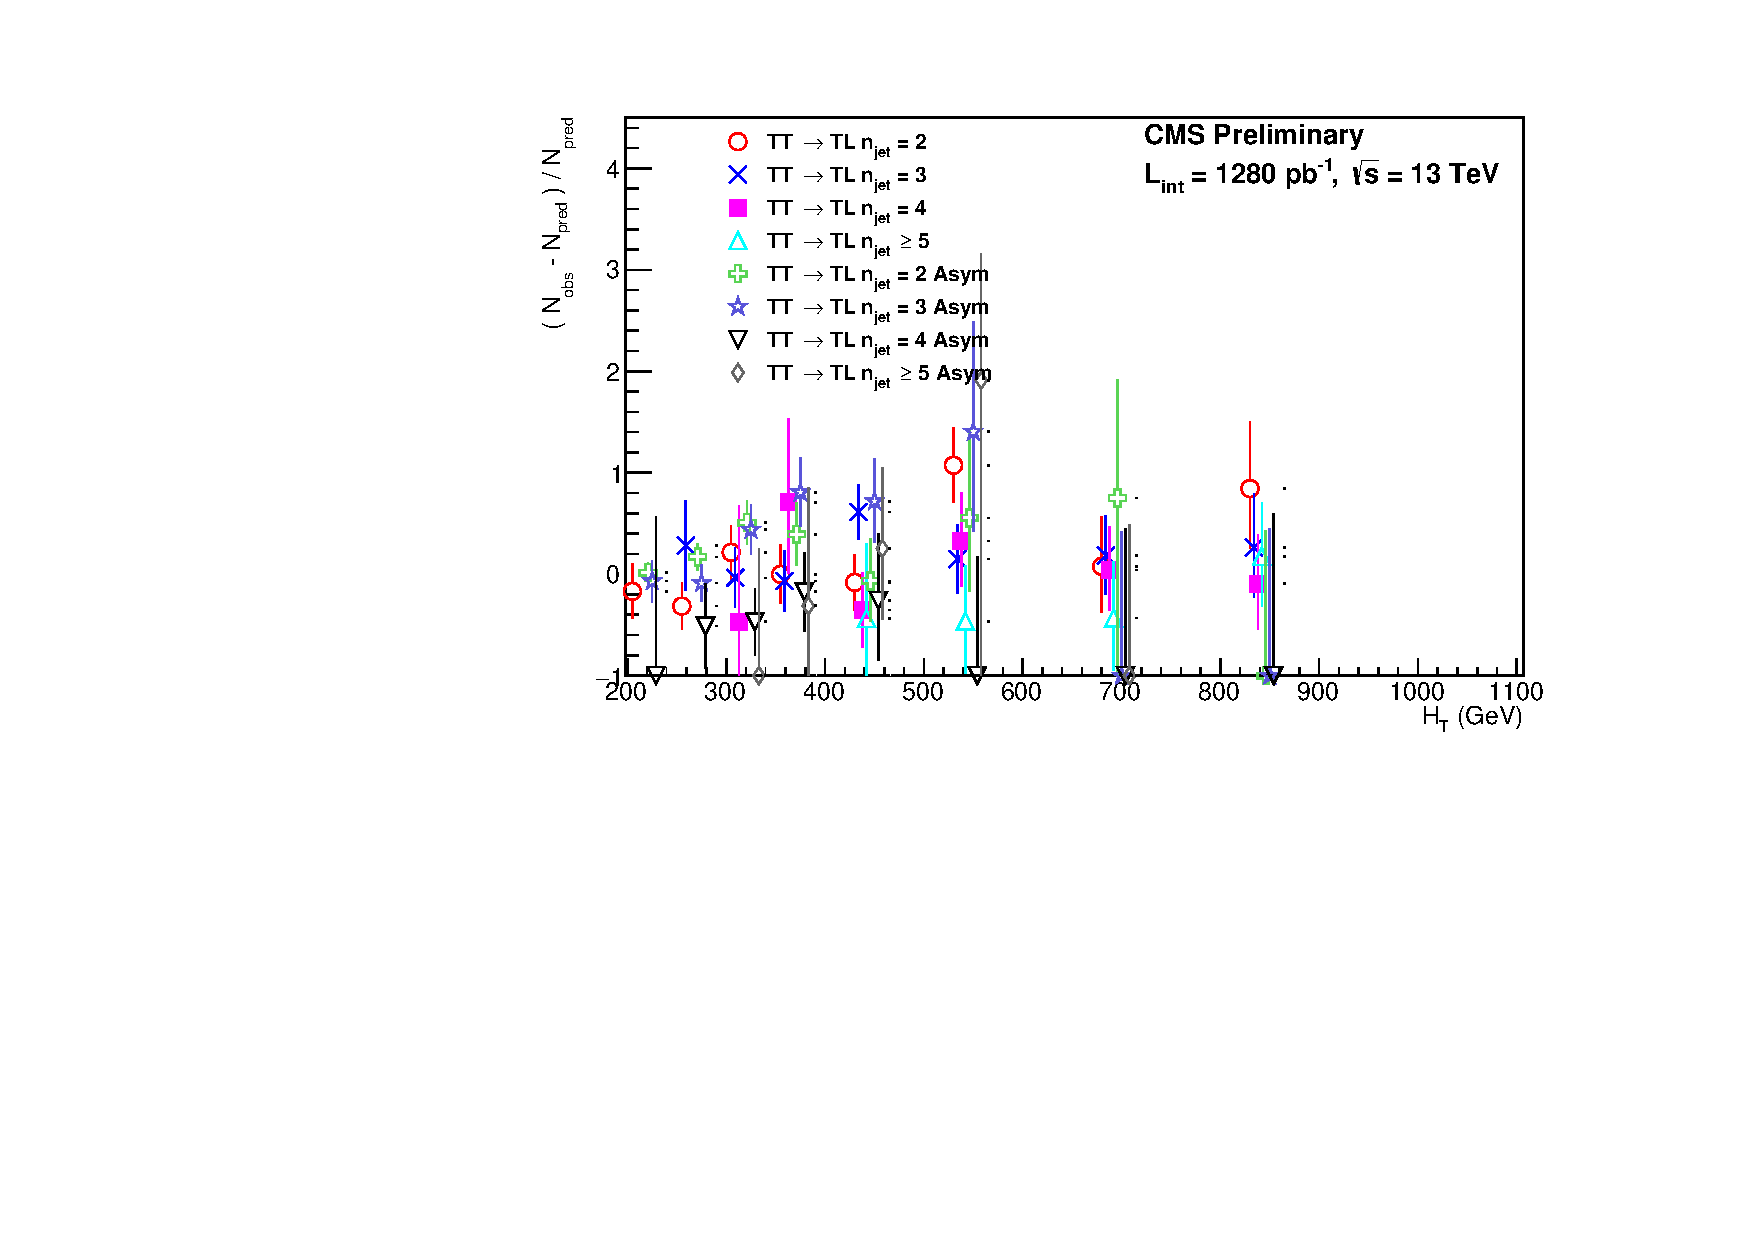
\includegraphics[width=0.6\textwidth]{figures/closureTests/newJamboree/looseLeptonCrossCheck.pdf}}
%     ~~
%     \subfigure[Pulls of closure
%     tests]{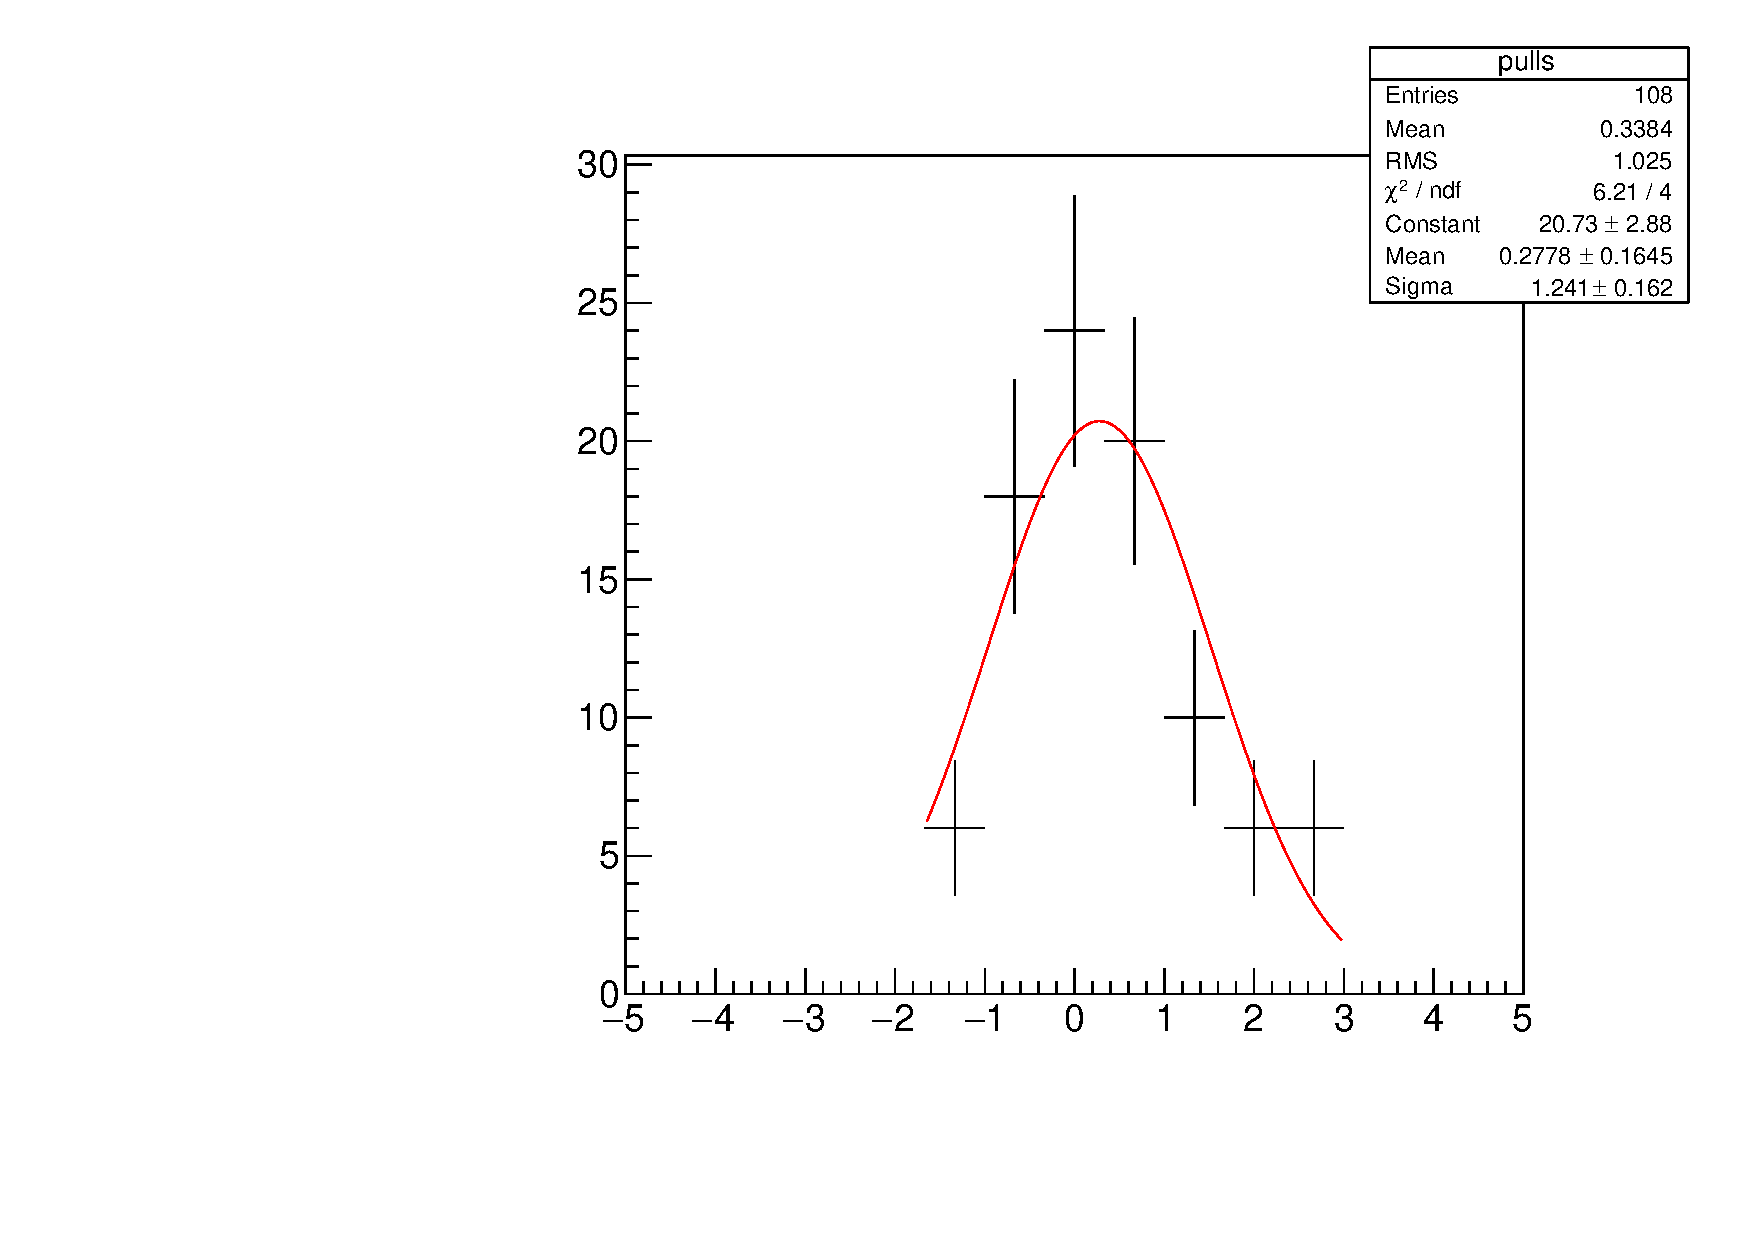
\includegraphics[width=0.4\textwidth]{figures/closureTests/newJamboree/looseLeptonPulls.pdf}} 
%     \caption{Closure tests probing the effect of lost leptons in the
%     analysis for each
%     \njet category (open symbols) and their pulls fit with a gaussian.
%     Carried out with $2.1\ifb$ of
%       $13\tev$ data. Events with two muons that pass the control
%       region (tight) muon criteria are used to predict events with one
%       tight muon and one muon that passes the signal region veto
%       criteria (loose)}
%     \label{fig:closureLooseLep}
%   \end{center} 
% \end{figure}

\subsection{Summary of normalisation systematic uncertainties based on $2.1~\ifb$}
\label{sec:closure-test-syst}

Normalisation systematics are derived from the MC studies and closure
test methods as described earlier in this section. The final numbers are summarised
in Table~\ref{tab:systs}. For the data-driven bins, in the kinematically restricted bins, such
as those with a high jet multiplicity and low value of \scalht, the
limited statistics leads to large systematic errors. In the bins populated 
with a reasonable number of events, the
systematic errors determined from the closure tests vary from $XX$ to
$XX\%$.

\begin{table}[h!]
  \caption{Systematic uncertainty ranges in the predictions
    of the $\ttbar$, W and $\znunu$  background
    components for each independent source of uncertainty considered.
    The data control samples correspond to an integrated
    luminosity of 2.1\fbinv. }\\
  \label{tab:systs}
  \centering
  \footnotesize
  \begin{tabular}{ ccccccccc }
    \hline
    \hline
    Systematic Source & \multicolumn{4}{c}{Transfer factor} \\
    
    (\njet,\nb,\scalht) & \mj to \zinv  & \mmj to \zinv & \gj to \zinv & \mj to W and \ttbar   \\
    \hline
    \alphat and \bdphi closure tests & $0.05-0.3$ & $0.05-0.3$ & - & $0.05-0.3$ \\
    \mj to \mmj closure tests & $0.1-0.25$ & - & - & - \\
    \gj to \mmj closure tests & - & - & $0.1-0.3$ & - \\
    0 b-tag to 1 b-tag closure tests & - & - & - & $0.05-1.0$ \\
    $\mu^+$ to $\mu^-$ closure tests & $0.05-0.5$ & - & - & $0.05-0.5$ \\
    Jet energy scale variations & $<0.1$ & $<0.1$ & $<0.1$ & $<0.1$ \\
    B-tag scale factor variations & $<0.05$ & $<0.02$ & $<0.02$ & $0.02-0.03$ \\
    Pileup weight variations & $0.01-0.02$  & $0.01-0.02$ & $0.01-0.02$ & $0.01-0.02$ \\
    Top $p_{T}$ reweighting variations & $<0.15$  & $<0.05$ & - & $<0.1$ \\
    Lepton scale factor variations & - & - & - & $0.01-0.03$ \\
    \hline
    \hline
  \end{tabular}
\end{table}

